%% abtex2-modelo-trabalho-academico.tex, v-1.9.2 laurocesar
%% Copyright 2012-2014 by abnTeX2 group at http://abntex2.googlecode.com/
%%
%% This work may be distributed and/or modified under the
%% conditions of the LaTeX Project Public License, either version 1.3
%% of this license or (at your option) any later version.
%% The latest version of this license is in
%%   http://www.latex-project.org/lppl.txt
%% and version 1.3 or later is part of all distributions of LaTeX
%% version 2005/12/01 or later.
%%
%% This work has the LPPL maintenance status `maintained'.
%%
%% The Current Maintainer of this work is the abnTeX2 team, led
%% by Lauro César Araujo. Further information are available on
%% http://abntex2.googlecode.com/
%%
%% This work consists of the files abntex2-modelo-trabalho-academico.tex,
%% abntex2-modelo-include-comandos and abntex2-modelo-references.bib
%%

% ------------------------------------------------------------------------
% ------------------------------------------------------------------------
% abnTeX2: Modelo de Trabalho Academico (tese de doutorado, dissertacao de
% mestrado e trabalhos monograficos em geral) em conformidade com
% ABNT NBR 14724:2011: Informacao e documentacao - Trabalhos academicos -
% Apresentacao
% ------------------------------------------------------------------------
% ------------------------------------------------------------------------

\documentclass[
	% -- opções da classe memoir --
	12pt,				% tamanho da fonte
	openright,			% capítulos começam em pág ímpar (insere página vazia caso preciso)
	twoside,			% para impressão em verso e anverso. Oposto a oneside
	a4paper,			% tamanho do papel.
	% -- opções da classe abntex2 --
	%chapter=TITLE,		% títulos de capítulos convertidos em letras maiúsculas
	%section=TITLE,		% títulos de seções convertidos em letras maiúsculas
	%subsection=TITLE,	% títulos de subseções convertidos em letras maiúsculas
	%subsubsection=TITLE,% títulos de subsubseções convertidos em letras maiúsculas
	% -- opções do pacote babel --
	english,			% idioma adicional para hifenização
	french,				% idioma adicional para hifenização
	spanish,			% idioma adicional para hifenização
	brazil				% o último idioma é o principal do documento
	]{abntex2}

% ---
% Pacotes básicos
% ---
\usepackage{lmodern}			% Usa a fonte Latin Modern
\usepackage[T1]{fontenc}		% Selecao de codigos de fonte.
\usepackage[utf8]{inputenc}		% Codificacao do documento (conversão automática dos acentos)
\usepackage{lastpage}			% Usado pela Ficha catalográfica
\usepackage{indentfirst}		% Indenta o primeiro parágrafo de cada seção.
\usepackage{color}				% Controle das cores
\usepackage{graphicx}			% Inclusão de gráficos
\usepackage{microtype} 			% para melhorias de justificação
\usepackage[final]{pdfpages}
\usepackage{url}
\usepackage{float}
\usepackage{amsmath}
\usepackage{cleveref}
\usepackage{pgfplots}
\pgfplotsset{compat=1.17}
\usepackage{amsfonts}
\usepackage{amsmath}
\usepackage{tikz}
\usetikzlibrary{matrix, positioning}
\usepackage{tabularx}
\usepackage{mathtools}
\usepackage{rotating}
\DeclareMathOperator{\logsumexp}{logsumexp}
\pgfmathdeclarefunction{sumexp}{3}{%
  \begingroup%
  \pgfkeys{/pgf/fpu}% "/pgf/fpu/output format=fixed" removed
  \pgfmathsetmacro{\myx}{#1}%
  \pgfmathtruncatemacro{\myxmin}{#2}%
  \pgfmathtruncatemacro{\myxmax}{#3}%
  \pgfmathsetmacro{\mysum}{0}%
  \pgfplotsforeachungrouped\XX in {\myxmin,...,\myxmax}%
    {\pgfmathsetmacro{\mysum}{\mysum+exp(\XX)}}%
  \pgfmathparse{\mysum+exp(#1)}%
  \pgfmathfloattofixed\pgfmathresult%  added
  \pgfmathsmuggle\pgfmathresult\endgroup%
}


\crefname{figure}{Figura}{Figuras}
\crefname{equation}{Equação}{Equações}
\crefname{table}{Tabela}{Tabelas}
% ---

% ---
% Pacotes adicionais, usados apenas no âmbito do Modelo Canônico do abnteX2
% ---
\usepackage{lipsum}				% para geração de dummy text
% ---

% ---
% Pacotes de citações
% ---
\usepackage[brazilian,hyperpageref]{backref}	 % Paginas com as citações na bibl
\usepackage[alf]{abntex2cite}	% Citações padrão ABNT

% ---
% CONFIGURAÇÕES DE PACOTES
% ---

% ---
% Configurações do pacote backref
% Usado sem a opção hyperpageref de backref
\renewcommand{\backrefpagesname}{Citado na(s) página(s):~}
% Texto padrão antes do número das páginas
\renewcommand{\backref}{}
% Define os textos da citação
\renewcommand*{\backrefalt}[4]{
	\ifcase #1 %
		Nenhuma citação no texto.%
	\or
		Citado na página #2.%
	\else
		Citado #1 vezes nas páginas #2.%
	\fi}%
% ---

% ---
% Informações de dados para CAPA e FOLHA DE ROSTO
% ---
\titulo{{Geração Procedural de Mapas para Jogos através da Segmentação de Imagens por Rede Neural Convolucional}}
\autor{Lucas da Silva dos Santos\\Matheus Zanivan Andrade\\ Rafael Nascimento Lourenço}
\local{São Paulo - Brasil}
\data{2023}
\orientador{Thyago Conchado Quintas}
% \coorientador{Equipe \abnTeX}
\instituicao{%
  Centro Universitário Senac - Santo Amaro
  \par
  Bacharelado em Ciência da Computação
}
\tipotrabalho{Trabalho de Conclusão de Curso (TCC)}
% O preambulo deve conter o tipo do trabalho, o objetivo,
% o nome da instituição e a área de concentração
\preambulo{Monografia apresentada na disciplina Trabalho de Conclusão de Curso, como parte dos requisitos para obtenção do título de Bacharel em Ciência da Computação.}
% ---


% ---
% Configurações de aparência do PDF final

% alterando o aspecto da cor azul
\definecolor{blue}{RGB}{41,5,195}

% informações do PDF
\makeatletter
\hypersetup{
     	%pagebackref=true,
		pdftitle={\@title},
		pdfauthor={\@author},
    	pdfsubject={\imprimirpreambulo},
	    pdfcreator={LaTeX with abnTeX2},
		pdfkeywords={abnt}{latex}{abntex}{abntex2}{trabalho acadêmico},
		colorlinks=true,       		% false: boxed links; true: colored links
    	linkcolor=blue,          	% color of internal links
    	citecolor=blue,        		% color of links to bibliography
    	filecolor=magenta,      		% color of file links
		urlcolor=blue,
		bookmarksdepth=4
}
\makeatother
% ---

% ---
% Espaçamentos entre linhas e parágrafos
% ---

% O tamanho do parágrafo é dado por:
\setlength{\parindent}{1.3cm}

% Controle do espaçamento entre um parágrafo e outro:
\setlength{\parskip}{0.2cm}  % tente também \onelineskip

% ---
% compila o indice
% ---
\makeindex
% ---

% ----
% Início do documento
% ----
\begin{document}

% Retira espaço extra obsoleto entre as frases.
\frenchspacing

% ----------------------------------------------------------
% ELEMENTOS PRÉ-TEXTUAIS
% ----------------------------------------------------------
% \pretextual

% ---
% Capa
% ---
\imprimircapa
% ---

% ---
% Folha de rosto
% (o * indica que haverá a ficha bibliográfica)
% ---
\imprimirfolhaderosto*
% ---

% ---
% Inserir a ficha bibliografica
% ---
% Isto é um exemplo de Ficha Catalográfica, ou ``Dados internacionais de
% catalogação-na-publicação''. Você pode utilizar este modelo como referência.
% Porém, provavelmente a biblioteca da sua universidade lhe fornecerá um PDF
% com a ficha catalográfica definitiva após a defesa do trabalho. Quando estiver
% com o documento, salve-o como PDF no diretório do seu projeto e substitua todo
% o conteúdo de implementação deste arquivo pelo comando abaixo:
%
% \begin{fichacatalografica}
%     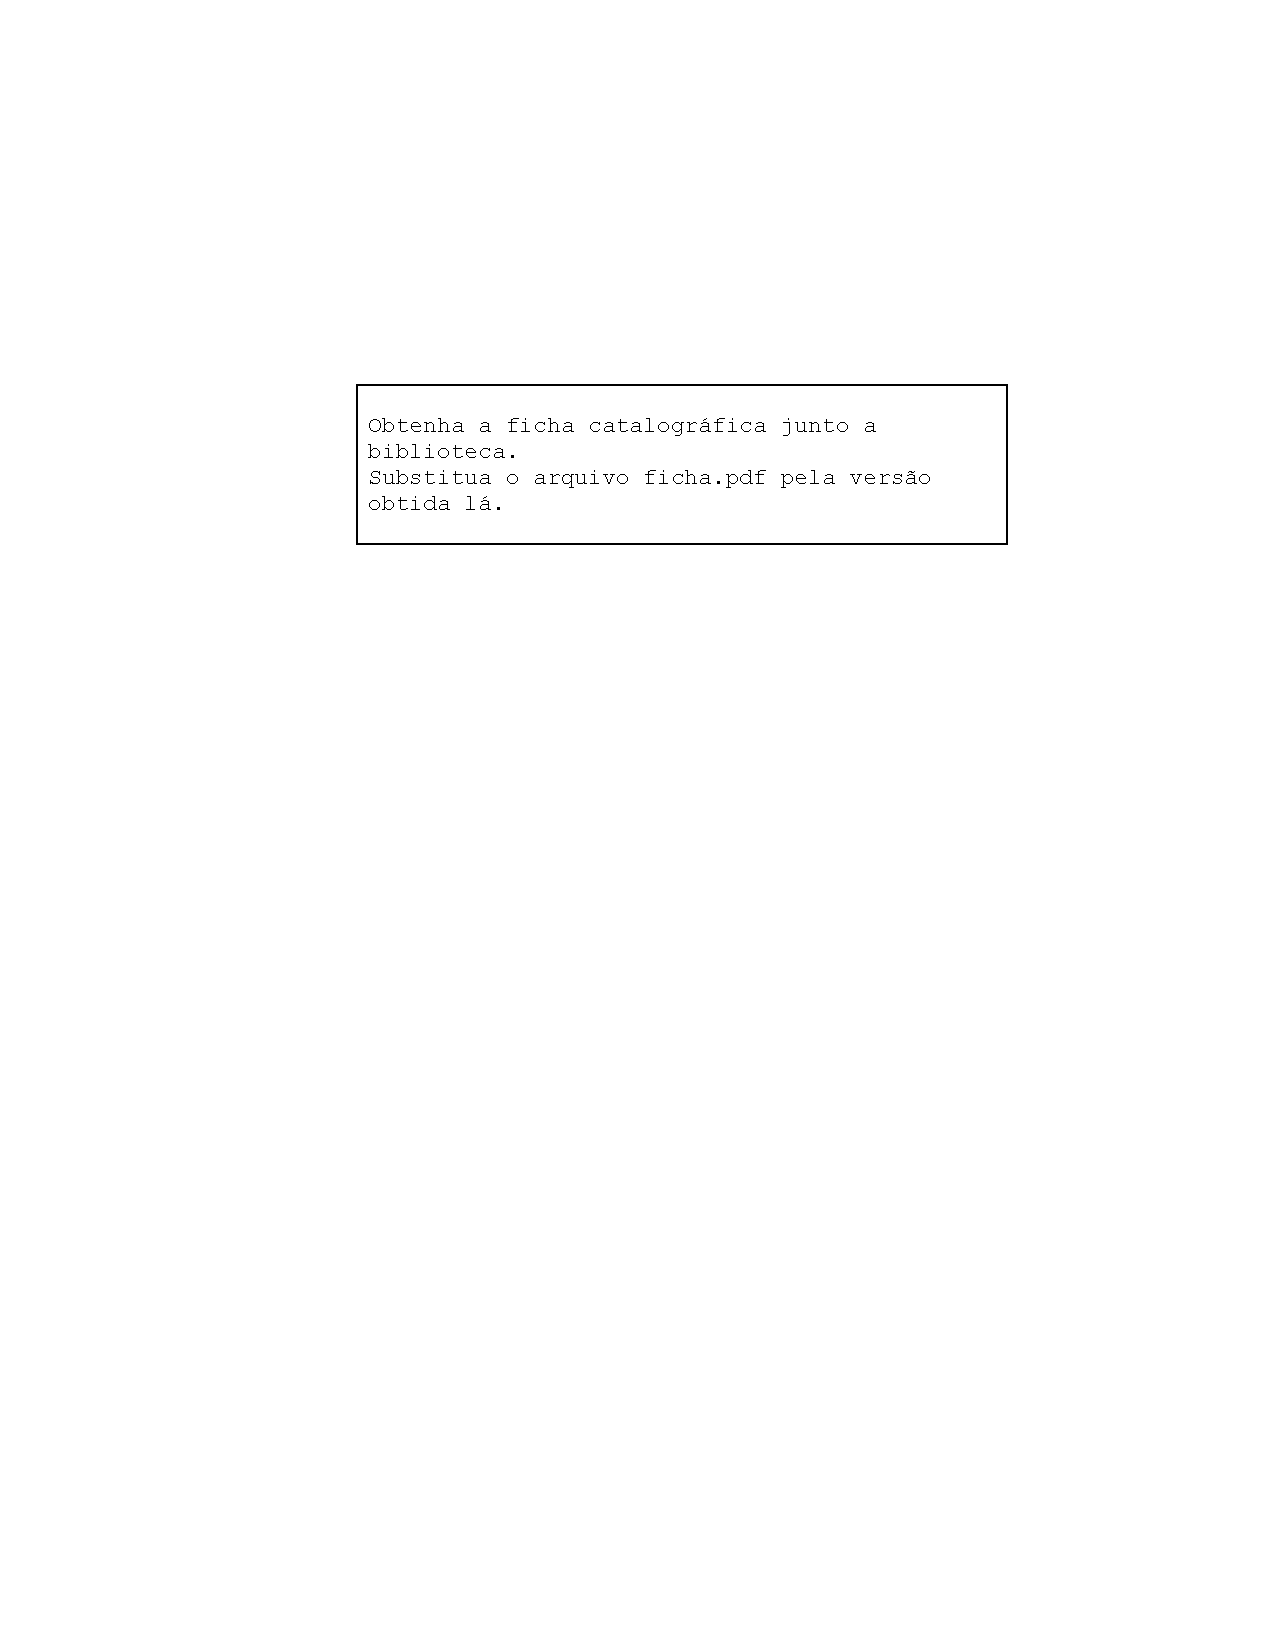
\includepdf{ficha.pdf}
% \end{fichacatalografica}
% ---

% ---
% Inserir errata
% ---
% \begin{errata}
% Elemento opcional da \citeonline[4.2.1.2]{NBR14724:2011}. Exemplo:

% \vspace{\onelineskip}

% FERRIGNO, C. R. A. \textbf{Tratamento de neoplasias ósseas apendiculares com
% reimplantação de enxerto ósseo autólogo autoclavado associado ao plasma
% rico em plaquetas}: estudo crítico na cirurgia de preservação de membro em
% cães. 2011. 128 f. Tese (Livre-Docência) - Faculdade de Medicina Veterinária e
% Zootecnia, Universidade de São Paulo, São Paulo, 2011.

% \begin{table}[htb]
% \center
% \footnotesize
% \begin{tabular}{|p{1.4cm}|p{1cm}|p{3cm}|p{3cm}|}
%   \hline
%    \textbf{Folha} & \textbf{Linha}  & \textbf{Onde se lê}  & \textbf{Leia-se}  \\
%     \hline
%     1 & 10 & auto-conclavo & autoconclavo\\
%    \hline
% \end{tabular}
% \end{table}

% \end{errata}
% ---

% ---
% Inserir folha de aprovação
% ---

% Isto é um exemplo de Folha de aprovação, elemento obrigatório da NBR
% 14724/2011 (seção 4.2.1.3). Você pode utilizar este modelo até a aprovação
% do trabalho. Após isso, substitua todo o conteúdo deste arquivo por uma
% imagem da página assinada pela banca com o comando abaixo:
%
% \includepdf{folhadeaprovacao_final.pdf}
%
\begin{folhadeaprovacao}

  \begin{center}
    {\ABNTEXchapterfont\large\imprimirautor}

    \vspace*{\fill}\vspace*{\fill}
    \begin{center}
      \ABNTEXchapterfont\bfseries\Large\imprimirtitulo
    \end{center}
    \vspace*{\fill}

    \hspace{.45\textwidth}
    \begin{minipage}{.5\textwidth}
        \imprimirpreambulo
    \end{minipage}%
    \vspace*{\fill}
   \end{center}

%    Trabalho aprovado. \imprimirlocal, 24 de novembro de 2012:

   \assinatura{\textbf{\imprimirorientador} \\ Orientador}
   \assinatura{\textbf{Professor} \\ Convidado 1}
   \assinatura{\textbf{Professor} \\ Convidado 2}
   %\assinatura{\textbf{Professor} \\ Convidado 3}
   %\assinatura{\textbf{Professor} \\ Convidado 4}

   \begin{center}
    \vspace*{0.5cm}
    {\large\imprimirlocal}
    \par
    {\large\imprimirdata}
    \vspace*{1cm}
  \end{center}

\end{folhadeaprovacao}
% ---

% ---
% Dedicatória
% ---
\begin{dedicatoria}
   \vspace*{\fill}
   \centering
   \noindent
   \textit{ Este trabalho é dedicado às crianças adultas que,\\
   quando pequenas, sonharam em se tornar cientistas.} \vspace*{\fill}
\end{dedicatoria}
% ---

% ---
% Agradecimentos
% ---
% \begin{agradecimentos}
% Os agradecimentos principais são direcionados à Gerald Weber, Miguel Frasson,
% Leslie H. Watter, Bruno Parente Lima, Flávio de Vasconcellos Corrêa, Otavio Real
% Salvador, Renato Machnievscz\footnote{Os nomes dos integrantes do primeiro
% projeto abn\TeX\ foram extraídos de
% \url{http://codigolivre.org.br/projects/abntex/}} e todos aqueles que
% contribuíram para que a produção de trabalhos acadêmicos conforme
% as normas ABNT com \LaTeX\ fosse possível.

% Agradecimentos especiais são direcionados ao Centro de Pesquisa em Arquitetura
% da Informação\footnote{\url{http://www.cpai.unb.br/}} da Universidade de
% Brasília (CPAI), ao grupo de usuários
% \emph{latex-br}\footnote{\url{http://groups.google.com/group/latex-br}} e aos
% novos voluntários do grupo
% \emph{\abnTeX}\footnote{\url{http://groups.google.com/group/abntex2} e
% \url{http://abntex2.googlecode.com/}}~que contribuíram e que ainda
% contribuirão para a evolução do \abnTeX.

% \end{agradecimentos}
% ---

% ---
% Epígrafe
% ---
% \begin{epigrafe}
%     \vspace*{\fill}
% 	\begin{flushright}
% 		\textit{``Não vos amoldeis às estruturas deste mundo, \\
% 		mas transformai-vos pela renovação da mente, \\
% 		a fim de distinguir qual é a vontade de Deus: \\
% 		o que é bom, o que Lhe é agradável, o que é perfeito.\\
% 		(Bíblia Sagrada, Romanos 12, 2)}
% 	\end{flushright}
% \end{epigrafe}
% ---

% ---
% RESUMOS
% ---

% resumo em português
\setlength{\absparsep}{18pt} % ajusta o espaçamento dos parágrafos do resumo
\begin{resumo}
  Esta monografia descreve o desenvolvimento de uma ferramenta para jogos que oferece uma nova funcionalidade. A ferramenta começa com a seleção de uma foto, que é processada por um modelo de rede neural convolucional especializado em segmentação panóptica. Isso permite a segmentação da imagem, incluindo a separação de objetos da mesma classe, como pessoas e carros. Após o modelo gerar a imagem de saída, será possível selecionar um contorno detectado e, a partir disso, gerar um mapa de forma procedural, combinado com o diagrama de Voronoi para criar os biomas do mapa. Além disso, será implementada uma automação no motor gráfico, incorporando um mapa jogável tridimensional e um minimapa bidimensional para geolocalização.

 \textbf{Palavras-chaves}: segmentação panóptica, geração procedural, diagrama de Voronoi, mapas, jogos.
\end{resumo}

% resumo em inglês
\begin{resumo}[Abstract]
 \begin{otherlanguage*}{english}
  This monograph describes the development of a tool for games that offers new functionality. The tool starts with the selection of a photo, which is processed by a convolutional neural network model specialized in panoptic segmentation. This allows for the segmentation of the image, including the separation of objects of the same class, such as people and cars. After the model generates the output image, it will be possible to select a detected outline and, from that, generate a procedural shape map, combined with the Voronoi diagram to create the biomes of the map.Furthermore, an automation will be implemented in the graphics engine, incorporating a playable three-dimensional map and a two-dimensional minimap for geolocation.

   \textbf{Key-words}: panoptic segmentation, procedural generation, Voronoi diagram, maps, games.
 \end{otherlanguage*}
\end{resumo}
% ---

% ---
% inserir lista de ilustrações
% ---
\pdfbookmark[0]{\listfigurename}{lof}
\listoffigures*
\cleardoublepage
% ---

% ---
% inserir lista de tabelas
% ---
\pdfbookmark[0]{\listtablename}{lot}
\listoftables*
\cleardoublepage
% ---

% ---
% inserir lista de abreviaturas e siglas
% ---
\begin{siglas}
  \item[IA] Inteligência Artificial
  \item[RGB] Red, Green and Blue ou Vermelho, Verde e azul
  \item[RNC] Rede Neural Convolucional
  \item[CNN] Convolutional Neural Network
  \item[RTC] Rede Totalmente Convolucional
  \item[RoI] Region of Interest ou Região de interesse
  \item[IoU] Intersection over Union ou União sobre intersecção
  \item[RPC] Pirâmide de Características
  \item[ECLE] Extrator de Características em Larga Escala
  \item[RPR] Rede de Proposta de Região
\end{siglas}
% ---

% ---
% inserir lista de símbolos
% ---
% \begin{simbolos}
%   \item[IA] inteligência Artificial
% \end{simbolos}
% ---

% ---
% inserir o sumario
% ---
\pdfbookmark[0]{\contentsname}{toc}
\tableofcontents*
\cleardoublepage
% ---



% ----------------------------------------------------------
% ELEMENTOS TEXTUAIS
% ----------------------------------------------------------
\textual

% ----------------------------------------------------------
% Introdução (exemplo de capítulo sem numeração, mas presente no Sumário)
% ----------------------------------------------------------
\chapter{Introdução}
% ----------------------------------------------------------

% introduzindo a jogos, por que é um mercado que está tao em alta
A indústria de jogos digitais cresce cada vez mais. De acordo com \citeonline{quanto_games_vao_movimentar}, essa indústria tende a ultrapassar em 2023, os US\$ 200 bilhões (aproximadamente, R\$ 1 trilhão). Novos jogos são produzidos e publicados diariamente, e somente na plataforma digital Steam, foram 10.644 novos títulos em 2022 como podemos ver na \cref{fig:steam_publishes} \space
% \cite{número_de_jogos_publicados_na_steam}.

\begin{figure}[!ht]
	\centering
    \caption{número de jogos publicados na Steam.}
	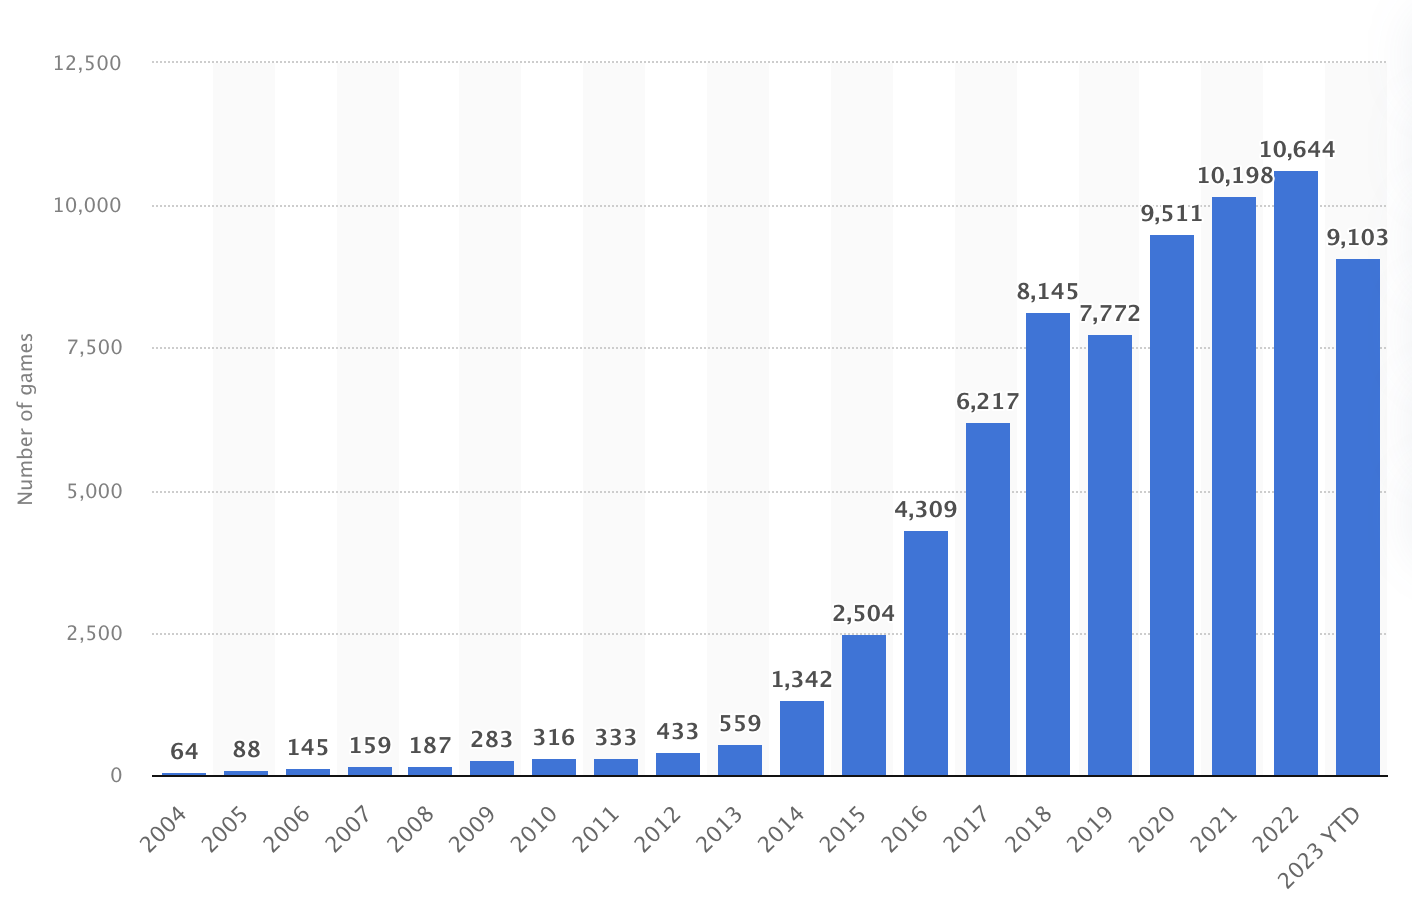
\includegraphics[width=0.6\textwidth]{figures/steam_sales.png}
	\legend{Fonte: \citeonline{numero_de_jogos_publicados_na_steam}}
	\label{fig:steam_publishes}
\end{figure}


% aqui a gente aproveita que falou de jogos para introduzir MAPAS que é o 'tema' do tcc
No cenário de jogos, os mapas desempenham um papel fundamental, fornecendo orientação aos jogadores e criando a sensação de escala em uma área. Por exemplo o jogo de aventura pirata chamado Sea of Thieves, os mapas revelam locais de interesse, como tesouros escondidos, missões e áreas perigosas, além de ajudar os jogadores a planejar suas estratégias, explorar o mundo virtual e tomar decisões com base em informações espaciais. Portanto os mapas enriquecem a experiência geral do jogo, mas cria-los pode ser um desafio, especialmente levando em consideração o orçamento disponível. Pois demandaria muitos recursos criar vários mapas diferentes com intuito de entretenimento do jogador. Em jogos como Minecraft, um elemento importante é a geração procedural, que consiste em um conjunto de algoritmos e ferramentas para geração de conteúdo, no qual se cria os mundos, com ilhas contendo biomas, cavernas, vilas, dentre outros recursos. Com essa diversidade de características pode-se evitar o tédio de sempre jogar no mesmo mapa \space\cite{video-game-maps, lecafedugeek}.

% \begin{figure}[ht]
% 	\caption{Mapa de tesouro do jogo Sea of Thieves}
% 	\centering % para centralizarmos a figura
% 	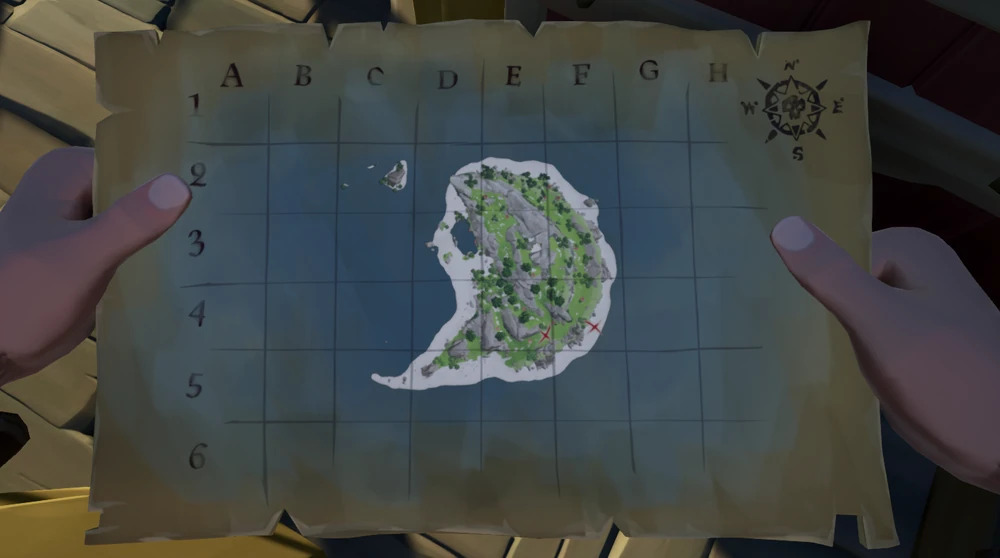
\includegraphics[width=10cm]{figures/Treasure_Map.jpg} % leia abaixo
% 	\legend{Fonte: \citeonline{seaofthieves}}
% 	\label{fig:treasureMap}
% \end{figure}

% aqui a gente faz um adendo e a demanda de jogos tende a crescer, então da a entender que você tem que produzir cada vez mais
% e também fala o quanto custa para produzir um jogo
% Ademais, o mercado de jogos no Brasil teve um aumento de 2,5\% em 2022, como apontado por uma pesquisa sobre o crescimento da demanda \space \space\cite{pesquisa_games_brasil}. O custo de produção de jogos varia bastante, dependendo do tamanho e da complexidade do projeto, \emph{e.g.}, a empresa Rockstar Games revelou que o jogo \textit{Grand Theft Auto V} custou cerca de 265 milhões de dólares para ser desenvolvido e comercializado \space \space\cite{gta_quanto_custou}.

%solução para o problema
% Apesar do rápido crescimento da indústria, existe uma carência de ferramentas que possam auxiliar os designers e artistas durante o processo de produção de jogos, o que acaba tornando-o demorado e, consequentemente, mais caro.  Segundo o livro "Procedural Content Generation in Games" \space\cite{procedural_centent_book}, uma abordagem eficiente para reduzir os custos de produção de um jogo é utilizar a geração procedural de conteúdo. Essa técnica permite maximizar o desenvolvimento de um jogo, envolvendo o uso de um software de computador capaz de criar conteúdo de jogos automaticamente. Esse software possibilita a geração automatizada de mapas, otimizando o processo de desenvolvimento.


% No entanto, a criação de mapas usando esse método ainda encontram dificuldades, sendo elas, variedade e autenticidade \space\cite{geracao_procedural_jogos_2d}.
% aqui adicionar uma explicação do porque é um desafio a geração procedural de conteúdo

Contextualizando, a área de Geometria Computacional é um ramo da ciência da computação que estuda algoritmos e estruturas de dados, servindo para resolução computacional de problemas geométricos. O diagrama de Voronoi é um dos tópicos mais discutidos dessa
área e possui uma gama de utilizações, dentre elas pode ser utilizado para resolver alguns problemas relacionados a jogos como por exemplo marcar pontos no mapa, desses pontos criar regiões, e a partir dessas regiões criar biomas gerando um mapa \space\cite{rodrigues_diagrama_2019}.


% introduz a relação de ia para personalização dentro de métodos procedurais em jogos
De acordo com \citeonline{jogo_procedural} é muito comum usar técnicas procedurais combinado com Inteligência Artificial (IA) para melhorar ou personalizar a experiência do jogador. Por exemplo, o jogo RimWorld é um simulador de colônia que gera um planeta de forma procedural e utiliza uma IA para narrar a história, abrangendo psicologia, ecologia, combate e diplomacia, dentre outros. Logo, essa combinação entre IA e a geração procedural cria uma jogabilidade única ao jogador.

% A aplicação da IA em jogos não se limita apenas à jogabilidade. Ela também é usada em áreas como animação de personagens, reconhecimento de fala e expressões faciais, tradução automática de idiomas nos diálogos do jogo e muito mais. A IA está impulsionando a inovação e a evolução dos jogos, proporcionando experiências cada vez mais envolventes e cativantes para os jogadores \space\cite{exameNvidia, omniverseace}.

% introduz o ramo de segmentação geral que será explicado mais para frente
Em IA, um ramo que está em ascensão é o de segmentação de imagem com redes neurais convolucionais, que constitui-se em classificar os pixeis de uma imagem ou criar áreas na imagem para destacar cada objeto (todas classes que são contáveis como pessoas, carros, etc) detectado ou até mesmo mesclar essas duas técnicas. Neste ramo existem diversas aplicações, como por exemplo carros autônomos e sistemas de vigilância.
Na aplicação de carros autônomos é necessário identificar humanos para tomar decisões de freio, em sistemas de vigilância é necessário identificar para alertar e automatizar o processo de segurança. Portanto, nessas aplicações reais observa-se a importância em identificar seres humanos para a tomada de decisões \space\cite{dp_semantic_segmantation}.

% Nessas aplicações é possível observar que é preciso ter um foco em identificar e segmentar seres humanos, por exemplo, em carros autônomos é primordial essa tarefa para o carro tomar a decisão de frear quando estiver muito perto de bater.

% Logo, se torna um tópico relevante dentro de visão computacional, no qual pode ter diversas aplicações no mundo real \space\cite{kirillov2019panoptic, dp_semantic_segmantation}.

Com base na contextualização é possível perceber que o mercado de jogos está em ascensão, o mapa é um recurso importante e pode ser usado a técnica de geração procedural para diversificar, o diagrama de Voronoi pode ser usado para gerar biomas em mapas no processo de geração procedural, a técnica de geração procedural de conteúdo unido a inteligência artificial é muito utilizado em jogos para criar personalizações, no ramo de inteligência artificial a segmentação com redes neurais convolucionais está em destaque. Logo pode-se perceber a relevância desses temas no curso de ciência da computação e na atualidade, propõe-se então, uma solução para personalizar mapas de jogos utilizando um modelo de IA da área de segmentação usando redes neurais convolucionais.

Com o objetivo de gerar mapas com biomas de forma procedural com personalização de IA, decidiu-se utilizar o resultado da segmentação de imagem por rede neural convolucional para o usuário selecionar uma área e assim delimitar o contorno da ilha, adicionando, portanto, uma personalização. Essa aplicação possibilita um desenvolvedor de jogos criar um protótipo de mapa rapidamente ou aprimorar e usar esse recurso no jogo, possibilitando o jogador tirar ou selecionar uma foto e escolher um contorno para gerar um mapa com aquele formato.

Por fim, para contribuição científica tem-se a hipótese de que quanto mais pontos o diagrama de Voronoi tiver maior será a precisão da compatibilidade entre o mapa gerado e o contorno escolhido. Para chegar a essa conclusão, comprometeu-se definir alguns testes com métricas em prol de mensurar a qualidade da geração procedural com o contorno selecionado.


% Por conseguinte, a combinação entre inteligência artificial e geração procedural de mapas pode abrir novas possibilidades de personalização nos jogos. Imagine um jogo em que, a partir da segmentação de imagens por meio de redes neurais convolucionais, os jogadores possam criar mapas únicos e personalizados para suas aventuras. Com uma foto, o modelo treinado segmentaria a imagem para selecionar um contorno reconhecido, e a partir dele se criar um mapa de maneira procedural contendo biomas no mesmo formato escolhido.

% No contexto da geração procedural de mapas, explorar a relação entre IA e personalização de jogos contribuirá para o avanço dessas áreas de pesquisa, proporcionando aos jogadores experiências mais ricas e variadas.

% Adicionar uma parte explicando a parte de visão computacional e porque o tema da nossa Ia é identificação de pessoas

% Dito isso, nosso projeto tem a ideia de fornecer recursos baseados em matemática aplicada dentro de ciência da computação que proporcione uma funcionalidade de escolher o contorno do mapa no qual irá jogar através de imagens. Abordaremos a arquitetura de redes neurais convolucionais, que é muito utilizada para trabalhar com imagens. Mais especificamente, abordaremos uma arquitetura derivada da arquitetura mencionada anteriormente, específica para segmentação de imagens, o que possibilita classificar contornos em imagens.

\section{Objetivos}

O objetivo principal deste trabalho é desenvolver uma ferramenta que ofereça uma alternativa para a geração procedural de mapas de ilhas, utilizando o diagrama de Voronoi para a criar biomas. Além disso, pretende-se combinar segmentação com redes neurais convolucionais para permitir a personalização desses mapas. Essa ferramenta terá a capacidade de reconhecer os contornos reconhecidos (classificados no conjunto de dados, logo o resultado terá uma detecção abrangente dentro do escopo de classes obtidas) de uma imagem, e gerar um mapa com um mapa baseado nos limites do contorno escolhido.

Adicionalmente, os seguintes objetivos específicos serão abordados:

\begin{itemize}
	\item Selecionar e analisar conjuntos de dados contendo classes relevantes, como pessoas, carros, entre outros, para treinar um modelo de rede neural convolucional específico para segmentação de imagens.
	\item Utilizar algoritmos para criar diagramas de Voronoi.
	\item Aplicar um algoritmo para reconhecer a imagem com o contorno selecionado e gerar como resultado a imagem do mapa gerado.
	\item Utilizar o resultado da segmentação para selecionar indicar o que é terreno em cima do diagrama de Voronoi.
	\item Gerar os biomas no diagrama de Voronoi.
	\item Criar testes em prol de mensurar a semelhança entre o contorno do mapa gerado com o contorno escolhido.
\end{itemize}

% Outro cenário que está crescendo muito nos últimos anos é o da inteligência artificial, afirma \citeonline{Valente_2020} que no Brasil mais que dobrou o número contratações de desenvolvedores da área de 2015 até 2020. De acordo com \apud{johnson2023}{briggs2023} um relatório recente relata que 300 milhões de empregos podem ser afetados pela IA \emph{i.e.} 18\% ofício global pode ser automatizado. Outrossim \citeonline{europarl2020} diz que o tópico de inteligência artificial é uma prioridade para União Europeia por ser considerada primordial para transformação digital da sociedade.  Do mesmo modo, Bill Gates, um dos fundadores da Microsoft — uma das maiores empresas de tecnologia —, diz que "o desenvolvimento da inteligência artificial (IA) é o avanço tecnológico mais importante em décadas"\space
% \space\cite{inteligencia_artificial_e_avanco_bbc}.

\chapter{Fundamentação teórica}

Este capítulo apresenta os conceitos fundamentais necessários para a realização dos objetivos propostos na monografia. Os tópicos foram organizados na ordem em que são utilizados na ferramenta final. Primeiro, será apresentado o tópico de geração procedural para gerar o mapa requerido, o diagrama de Voronoi para ser aplicado como um filtro na imagem e aplicar os biomas. Em seguida, o conceito geral de visão computacional e por fim, serão apresentados os conceitos de inteligência artificial, tanto em um contexto amplo quanto em relação ao conteúdo proposto, que é a segmentação panóptica.

\section{Geração procedural de conteúdo}

Segundo \space\citeonline{yannakakis2018artificial}, em poucas palavras, a geração procedural de conteúdo constituí métodos e automações utilizados para gerar conteúdos em jogos. A geração procedural de conteúdo também é uma parte importante da inteligência artificial de um jogo e já vem sendo utilizada desde 1980.
Essa técnica pode ser utilizada para gerar níveis, mapas, textura, regras de jogo, historia, entre outras coisas.

É difícil dizer qual algoritmo foi utilizado para geração de conteúdo dos jogos modernos e os códigos fontes não são facilmente acessíveis. Já nos jogos antigos os códigos fontes e as estratégias utilizadas são acessíveis e muito bem documentadas na internet. São geralmente utilizados algoritmos de geração aleatória que podem ser classificados como sendo de força bruta, e são usados para criar estruturas ou mapas dependendo do tipo de jogo \space\cite{dormans2010adventures}.


\subsection{Diagrama de Voronoi}

Segundo \citeonline{rodrigues_diagrama_2019} diagrama de Voronoi é o particionamento do espaço onde cada região é associada a um ponto do conjunto.

O diagrama de Voronoi é gerado a partir das distancias euclidianas entre os vizinhos de um conjunto de pontos do plano\space
\cite{diagrama_de_voronoi:_uma_exploracao_nas_distancias_euclidiana_e_do_taxi}. Esse diagrama possui uma gama de utilizações, por exemplo, estudar epidemias, encontrar o 
ponto mais próximo, calcular a precipitação de uma área, estudar os padrões de crescimento das florestas, etc,\space\cite{poligonos_de_thiessen_ou_voronoi}. 

Seja um conjunto de índices $I_n = \{1, 2, 3, ..., n\}$ e $A = \{p_1, p_2, ..., p_n\} \subset \mathbb{R}^2$ um conjunto de pontos onde $2 \leq n < \infty$, definimos como região de Voronoi o conjunto de pontos associado a $p_i$, onde d é a distancia euclidiana

\begin{equation}
	V(p_i) = \{p|d(p_i,p) \leq d(p_i,p);i \neq j, i, j \in I_n\},
\end{equation}


temos o conjunto formado por essas regiões sendo $V(A) = {V(1), V(2), V(3), ..., V(n)}$ \cite{rodrigues_diagrama_2019}.

Na figura \cref{fig:diagrama_voronoi} podemos ver a relação do conjuntos de pontos com o diagrama de Voronoi.

\begin{figure}[H]
	\centering
	\caption{Diagrama de Voronoi.}
	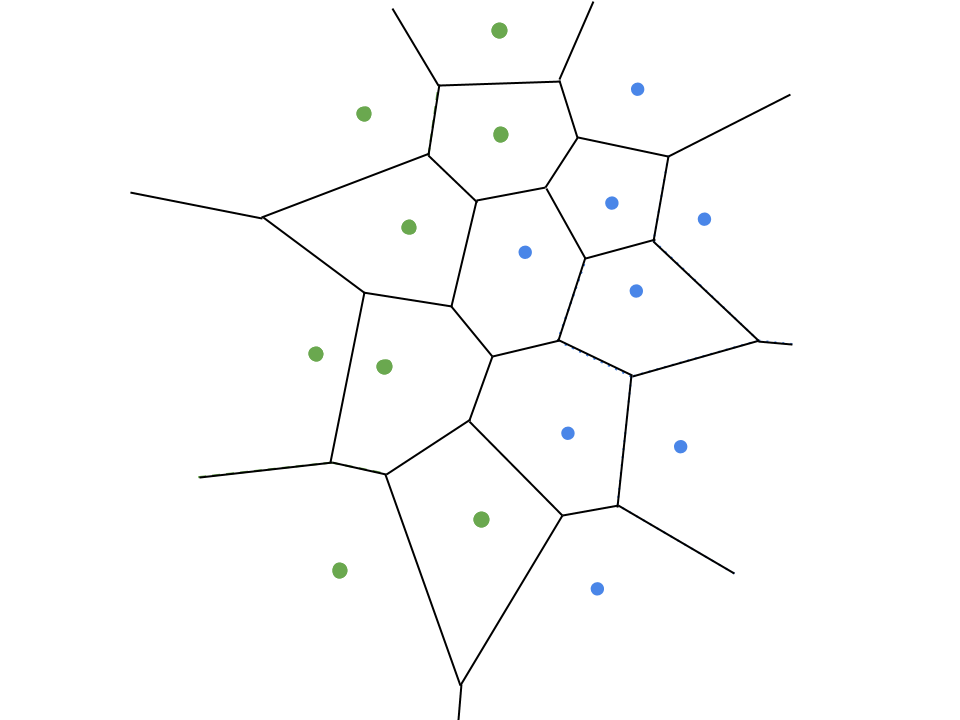
\includegraphics[width=0.8\textwidth]{figures/diagrama_de_voronoi.png}
	\legend{Fonte: \citeonline{thomazthz_diagrama_2014}}
	\label{fig:diagrama_voronoi}
\end{figure}


\subsection{Geração de biomas no diagrama de Voronoi}
\label{sec:geracaoProcedural}

Biomas são regiões ecológicas que possuem uma fauna e flora com atributos estruturais semelhantes \space\cite{maestrovirtuale}. Segundo \citeonline{amitp2010} o primeiro passo para gerar o mapa e os biomas é gerar o litoral, os litorais serão as bordas que irão dizer o que é água e o que é solo. Na \cref{fig:voronoi-land-water} mostra-se essa separação, sendo os polígonos pintados de marrom é o solo e o polígonos azuis representam o mar. Existem algumas formas de gerar o formato da ilha:

\begin{itemize}
    \item Radial: gera ilhas circulares através de ondas senoidais.
    \item Perlin: utiliza o Perlin Noise para controlar a forma da ilha.
    \item Quadrado: preenche o mapa inteiro com solo.
\end{itemize}

É possível utilizar qualquer formato para gerar as ilhas \space\cite{amitp2010}.

\begin{figure}[ht]
	\caption{Diagrama de Voronoi separado em solo e mar}
	\centering % para centralizarmos a figura
	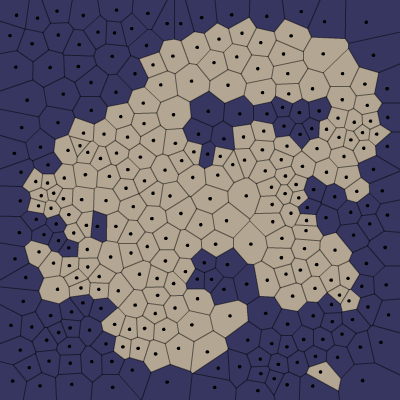
\includegraphics[width=0.8\textwidth]{figures/voronoi-land-water.png} % leia abaixo
	\legend{Fonte: \citeonline{amitp2010}}
	\label{fig:voronoi-land-water}
\end{figure}

O próximo passo é calcular a elevação do terreno. A elevação será calculada através da distancia de um polígono indicado como solo até o litoral, a elevação é definida pelos cantos dos polígonos \space\cite{amitp2010}. Na \cref{fig:downslopes}

\begin{figure}[ht]
	\caption{Diagrama de Voronoi separado em solo e mar com os cantos dos polígonos indicando a direção para o litoral}
	\centering
	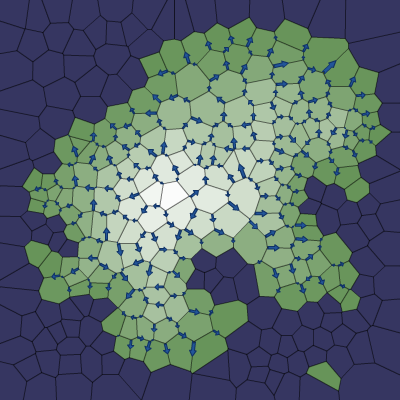
\includegraphics[width=0.7\textwidth]{figures/downslopes.png}
	\legend{Fonte: \citeonline{amitp2010}}
	\label{fig:downslopes}
\end{figure}

Com a elevação, é possível gerar os biomas. Um exemplo seria elevações altas significa que é uma montanha, logo ela deve possuir neve. Adicionando mais uma camada, além da elevação, como a de umidade, podemos gerar uma variedade maior de biomas. A umidade é calculada de quão longe o polígino está de um corpo d'água.

\subsection*{Diagrama de Whittaker}

O diagrama de Whittaker é uma forma de dividir os terrenos gerados a partir da técnica de geração procedural. Esse diagrama inclui valores de temperatura e umidade para separar os biomas, exemplificado na \cref{fig:diagrama-whittaker} \space\cite{wikidotwhittakerdiagram}.

\begin{figure}[ht]
	\caption{Diagrama de Whittaker}
	\centering
	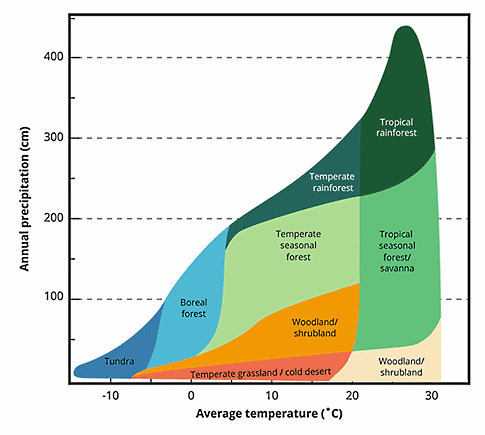
\includegraphics[width=0.6\textwidth]{figures/diagrama-whittaker.png}
	\legend{Fonte: \citeonline{mendes2019}}
	\label{fig:diagrama-whittaker}
\end{figure}

Usando a elevação como representante da temperatura de um bioma, é possível utilizar o diagrama de Whittaker. Fazendo alterações nesse diagrama, é possível adicionar ou remover biomas. Com essa nova camada possibilita a adição de rios ao mapa \space\cite{amitp2010} e assim obtendo o resultado apresentado na figura \ref{fig:biomes}.

\begin{figure}[ht]
	\caption{Resultado final da geração do mapa}
	\centering
	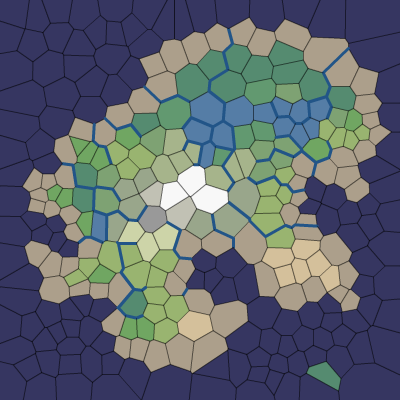
\includegraphics[width=0.5\textwidth]{figures/biomes.png}
	\legend{Fonte: \citeonline{amitp2010}}
	\label{fig:biomes}
\end{figure}




Para utilizar essa técnica de geração procedural de mapas, é necessário começar com uma imagem que sirva como base para a geração do mapa. É empregada a visão computacional para extrair dados da imagem.

\section{Visão computacional}

A visão computacional está em constante avanço, aproximando cada vez mais os computadores da capacidade visual humana. De acordo com Horst Haußecker e Bernd Jähne, no livro "Computer Vision and Applications" \cite{comp_vision_and_applications}, a visão computacional é uma área da computação que se dedica à interpretação de imagens por meio de algoritmos e técnicas de processamento de imagens. Essa área abrange a aquisição, processamento e análise de imagens, com o objetivo de extrair informações úteis para resolver problemas específicos.

Porém, segundo Richard Szeliski, no livro "Computer Vision: Algorithms and Applications" \cite{computer_vision_richard}, nas últimas décadas ocorreram avanços significativos na busca de aproximar a visão computacional da visão humana, porém não obteve total êxito. Isso ocorre porque, enquanto o olho humano enxerga com aparente facilidade as estruturas tridimensionais e suas nuances, a visão computacional depende de técnicas matemáticas altamente precisas para recuperar a forma tridimensional e a aparência dos objetos.

Nas figuras \cref{fig:imagem_a} e \cref{fig:imagem_b}, evidencia-se a notável capacidade de um computador em distinguir, classificar e até mesmo compreender os elementos presentes em uma fotografia.

\begin{figure}
    \centering
    \begin{minipage}[b]{0.49\textwidth}
      \centering
      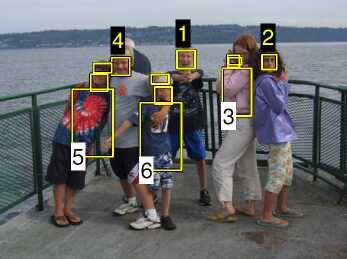
\includegraphics[width=0.6\textwidth]{figures/detectacao_de_faces_exemplo.JPG}
      \caption{Algoritmos de detecção facial e de roupas/cabelos por cor localizam e reconhecem pessoas nesta imagem \cite{computer_vision_richard}}
      \label{fig:imagem_a}
    \end{minipage}
    \hfill
    \begin{minipage}[b]{0.49\textwidth}
      \centering
      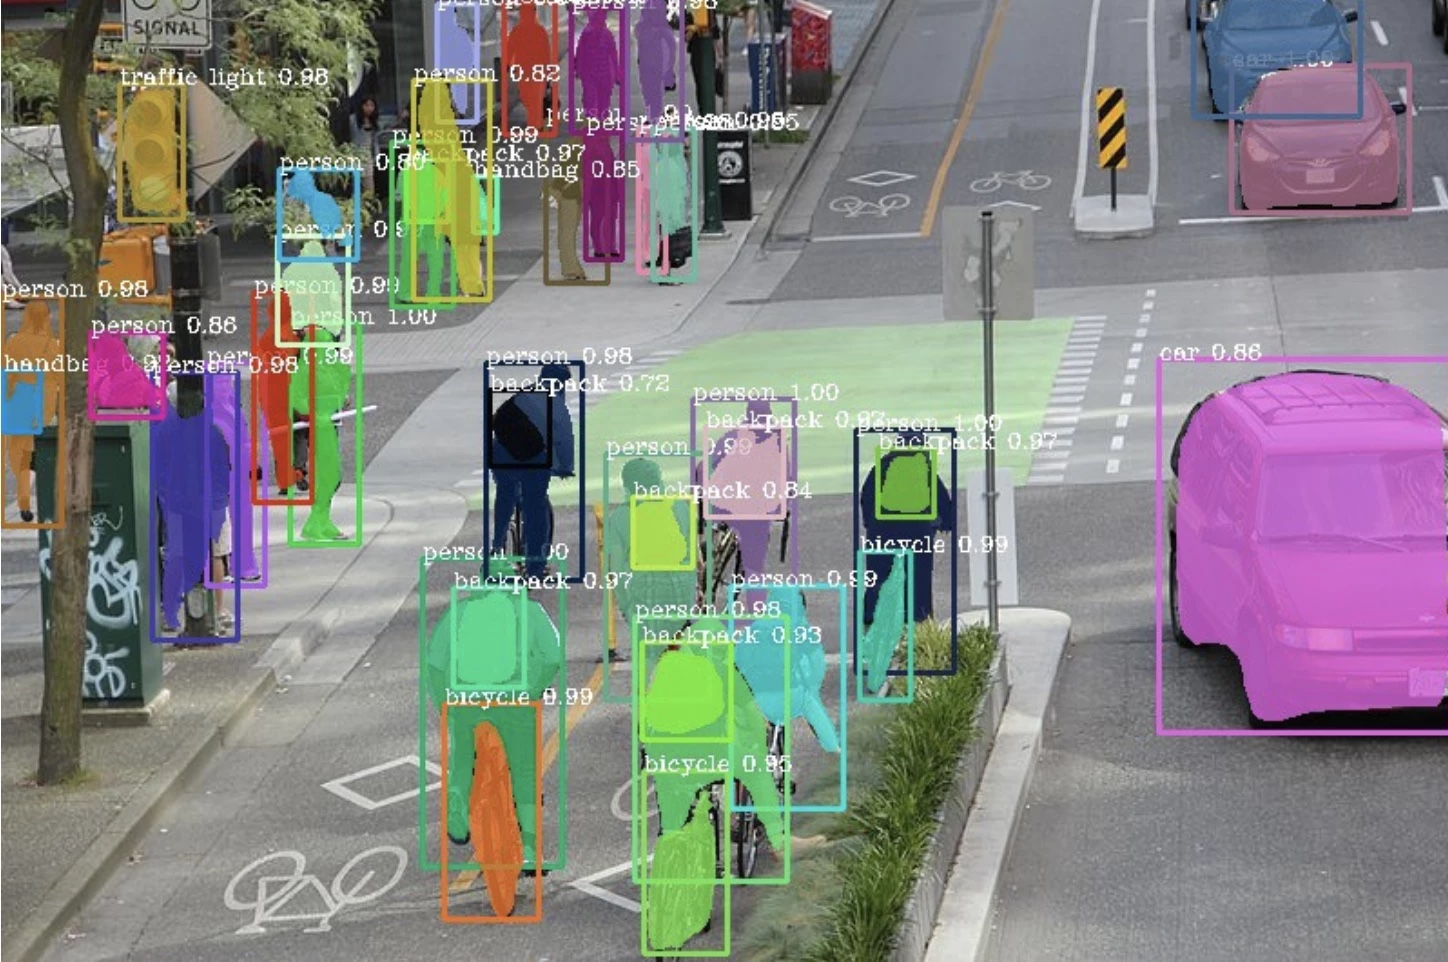
\includegraphics[width=0.6\textwidth]{figures/semantic_intance.JPG}
        \caption{Segmentação de instâncias de objetos pode delinear cada pessoa e objeto em uma cena complexa. 
        \cite{instance_segmentation}}
      \label{fig:imagem_b}
    \end{minipage}
  \end{figure}


No entanto, apesar do sucesso no uso dessas técnicas, o computador ainda não consegue oferecer a mesma quantidade de detalhes na explicação de uma imagem como o olho humano. Isso se deve à maior facilidade do computador em compreender linguagem em comparação à visualização. A tarefa de ensinar um computador a ver e descrever com precisão e riqueza de detalhes o que está sendo observado é extremamente complexa \cite{computer_vision_richard}.

A visão é um elemento crucial para capacitar a inteligência artificial a realizar diversas tarefas. A fim de replicar a visão humana, é necessário que as máquinas sejam capazes de adquirir, processar, analisar e compreender imagens. \cite{como_funciona_visao_computacional}

% Na \cref{fig:comp_vision} podemos ver uma analogia entre a forma como uma imagem é processada pelo cérebro humano e a forma como é processada por um sistema computacional.

% \begin{figure}[!ht]
% 	\centering
% 	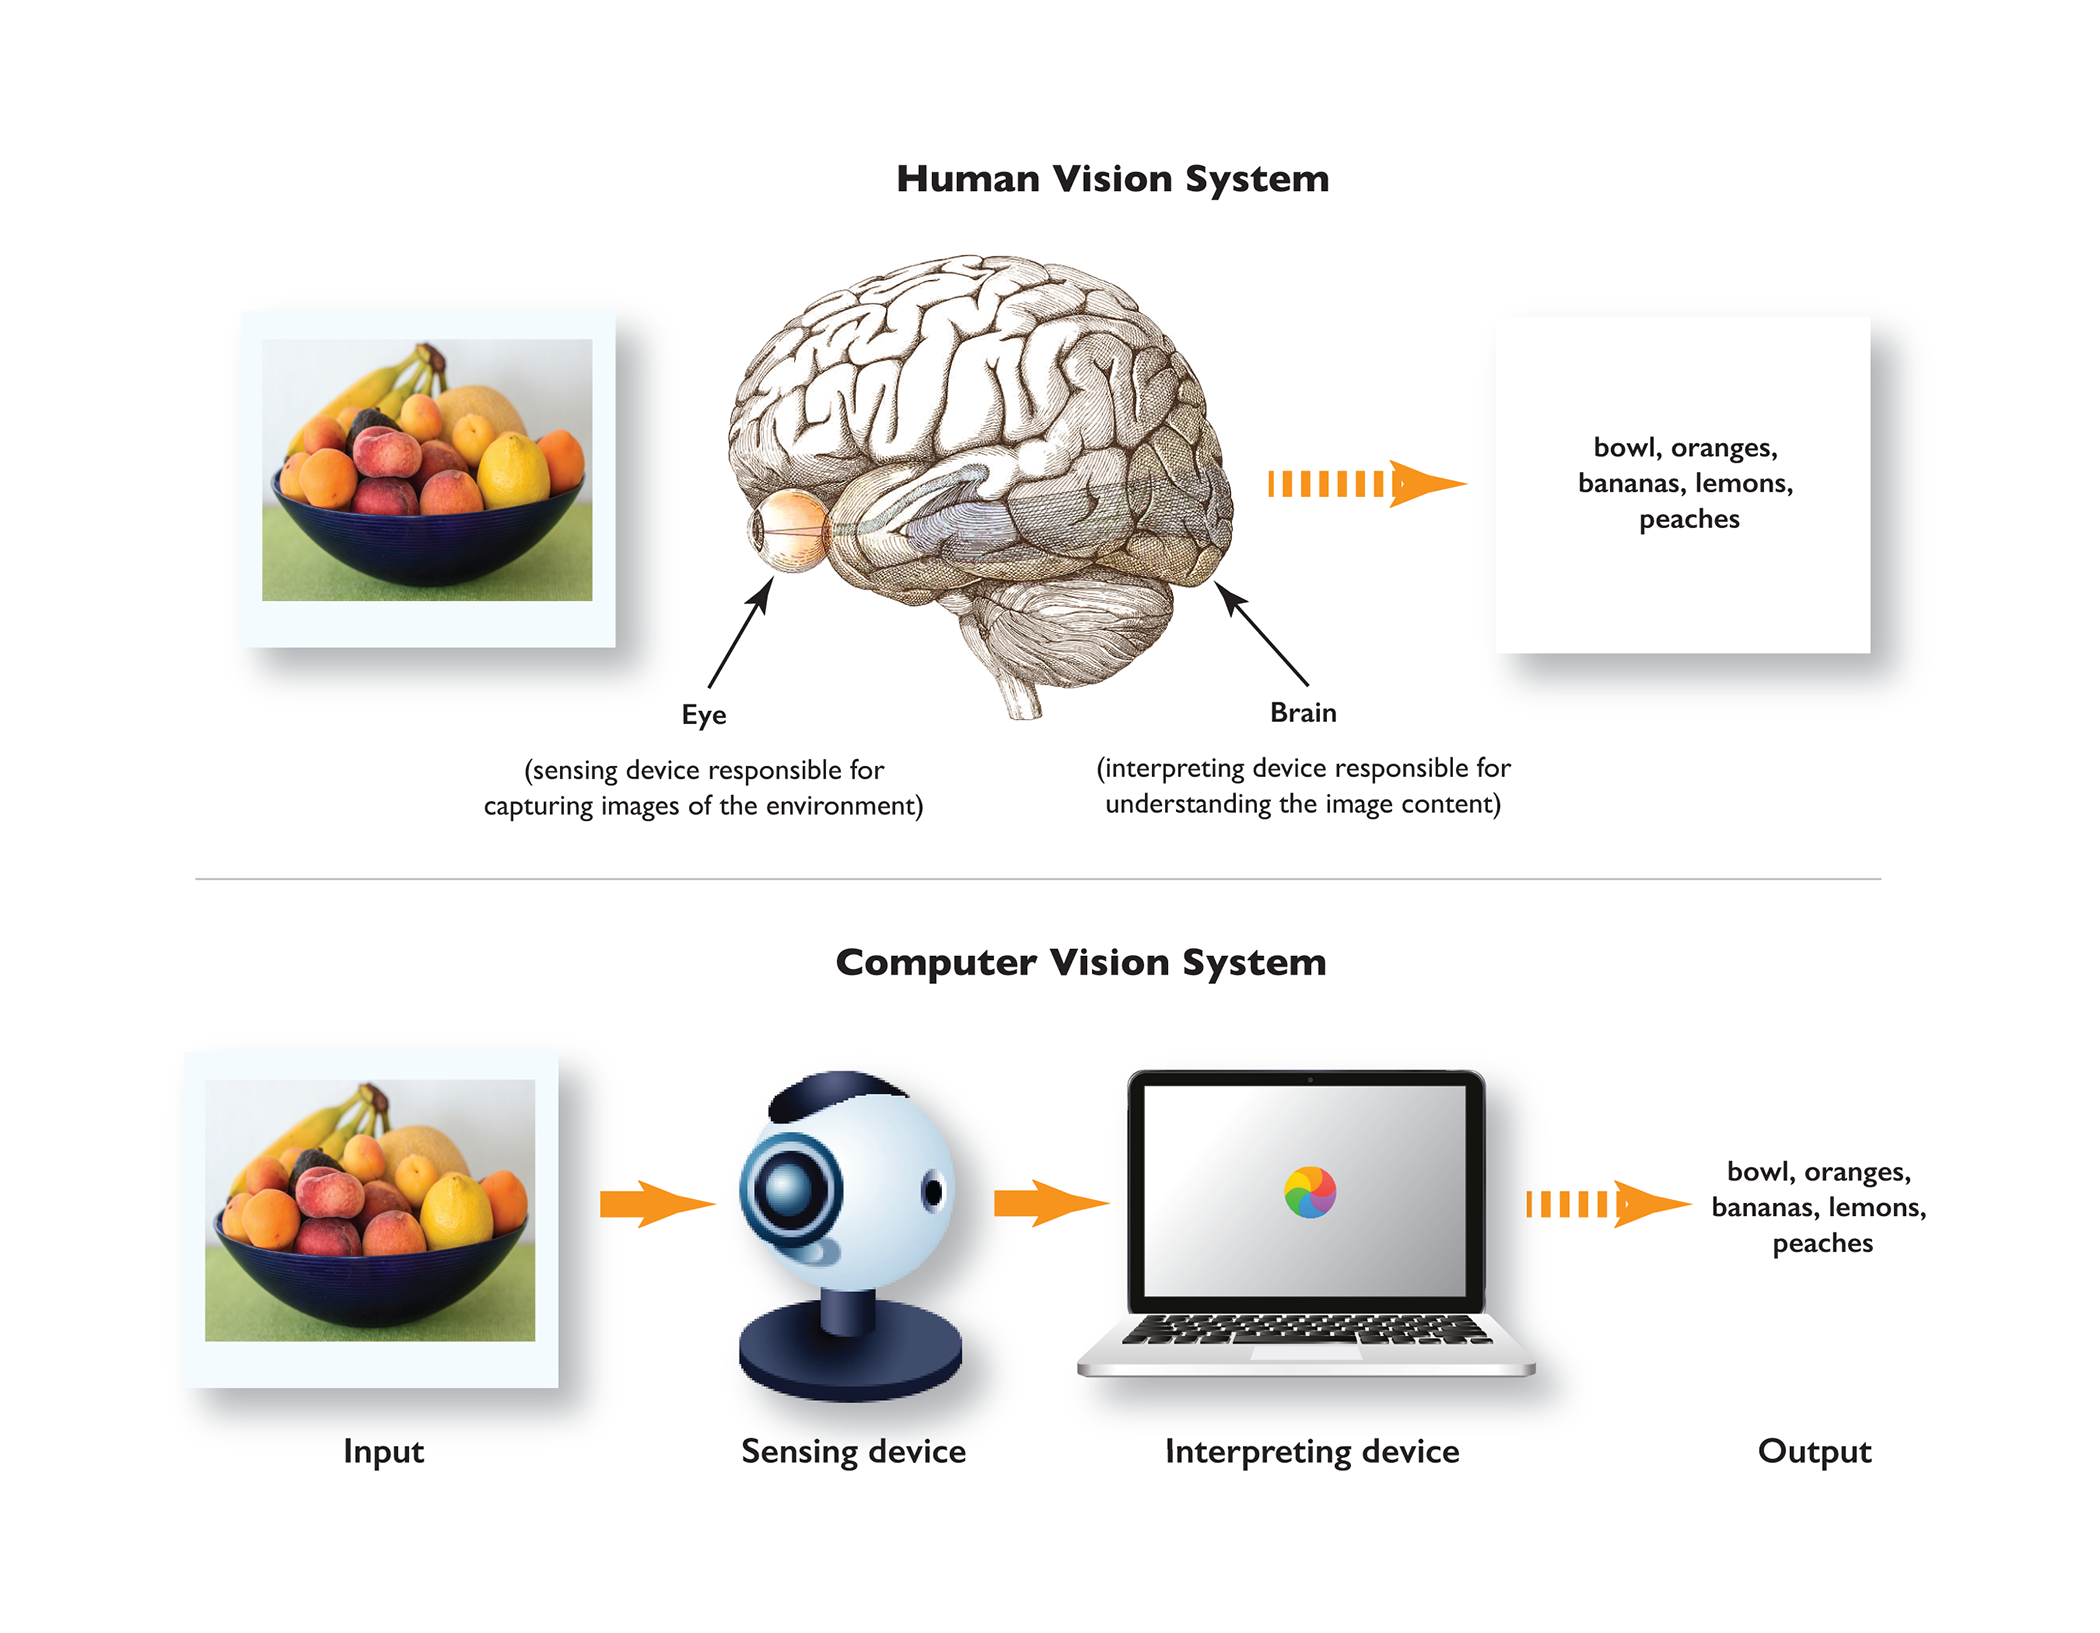
\includegraphics[width=0.6\textwidth]{figures/content_Human_Vision.png}
% 	\caption{Visão humana e sistemas de visão computacional processam dados visuais de maneira semelhante \cite{content_Human_Vision}.}
% 	\label{fig:comp_vision}
% \end{figure}	

No processamento de computação visual, as imagens são adquiridas e representadas como uma matriz 2D de pixels. Cada pixel corresponde a um ponto na imagem e é representado por um valor numérico que varia de 0 a 255. Esses valores de pixel descrevem a intensidade da cor em uma escala de cinza. Dessa forma, um computador interpreta uma imagem como uma matriz de números, permitindo que ele analise e compreenda os detalhes visuais presentes na imagem, como no caso da \cref{fig:comp_vision} do presidente dos Estados Unidos, Abraham Lincoln\cite{mit_video}.

Os algoritmos de visão computacional utilizados atualmente são fundamentados em reconhecimento de padrões. O procedimento consiste em treinar computadores por meio de uma vasta quantidade de dados visuais. Os computadores processam imagens, rotulam os objetos nelas contidos e identificam padrões entre esses objetos \cite{content_Human_Vision}.

Esse processo de treinamento e reconhecimento de padrões permite que os computadores identifiquem objetos e compreendam seu contexto visual. Com essa capacidade, o computador consegue realizar tarefas como, por exemplo, reconhecimento facial \cref{fig:imagem_a}.

\begin{figure}[!ht]
	\centering
	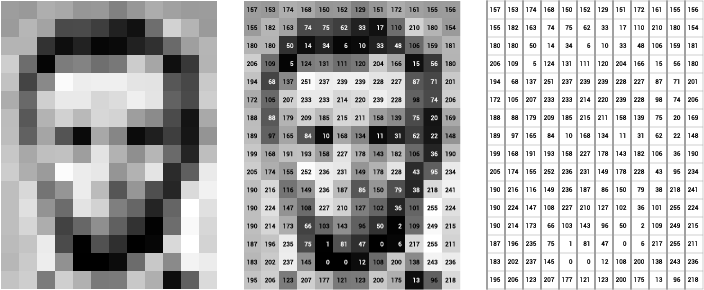
\includegraphics[width=0.6\textwidth]{figures/lincoln_pixel_values.png}
	\caption{Diagrama de dados de pixels. À esquerda, nossa imagem de Lincoln; no centro, os pixels rotulados com números de 0 a 255, representando sua luminosidade; e à direita, apenas esses números \cite{content_Human_Vision}.}
	\label{fig:comp_vision}
\end{figure}





É bastante comum na área de visão computacional contarmos com o auxílio de algoritmos de inteligência artificial que capacitam o computador a reconhecer padrões e características nas imagens processadas.

\section{Inteligência Artificial}
Inteligência artificial é uma técnica científica que simula o pensamento humano de forma que possa ser executado em uma máquina, podendo ser utilizada para criar soluções com uma linha de progressão parecida ao raciocínio lógico como conhecemos. Isto permite ao computador reconhecer e interpretar o mundo ao redor com imagens e textos criando uma ampla área de atuação que otimiza tarefas antes só realizadas por seres humanos \space\cite{ia_aliada_ou_inimiga}.

Este ramo é complexo por se tratar de uma representação cognitiva, se torna necessário usar uma base com diversas áreas científicas como psicologia, biologia, lógica matemática, linguística, engenharia, filosofia, entre outras. E pode ser usado para diversos problemas específicos como, por exemplo, definir as boas rotas para algum processo logístico \space\cite{ia_conceitos_aplicacoes}.

\begin{figure}[H]
	\caption{Diagrama de aprendizado de máquina}
	\centering % para centralizarmos a figura
	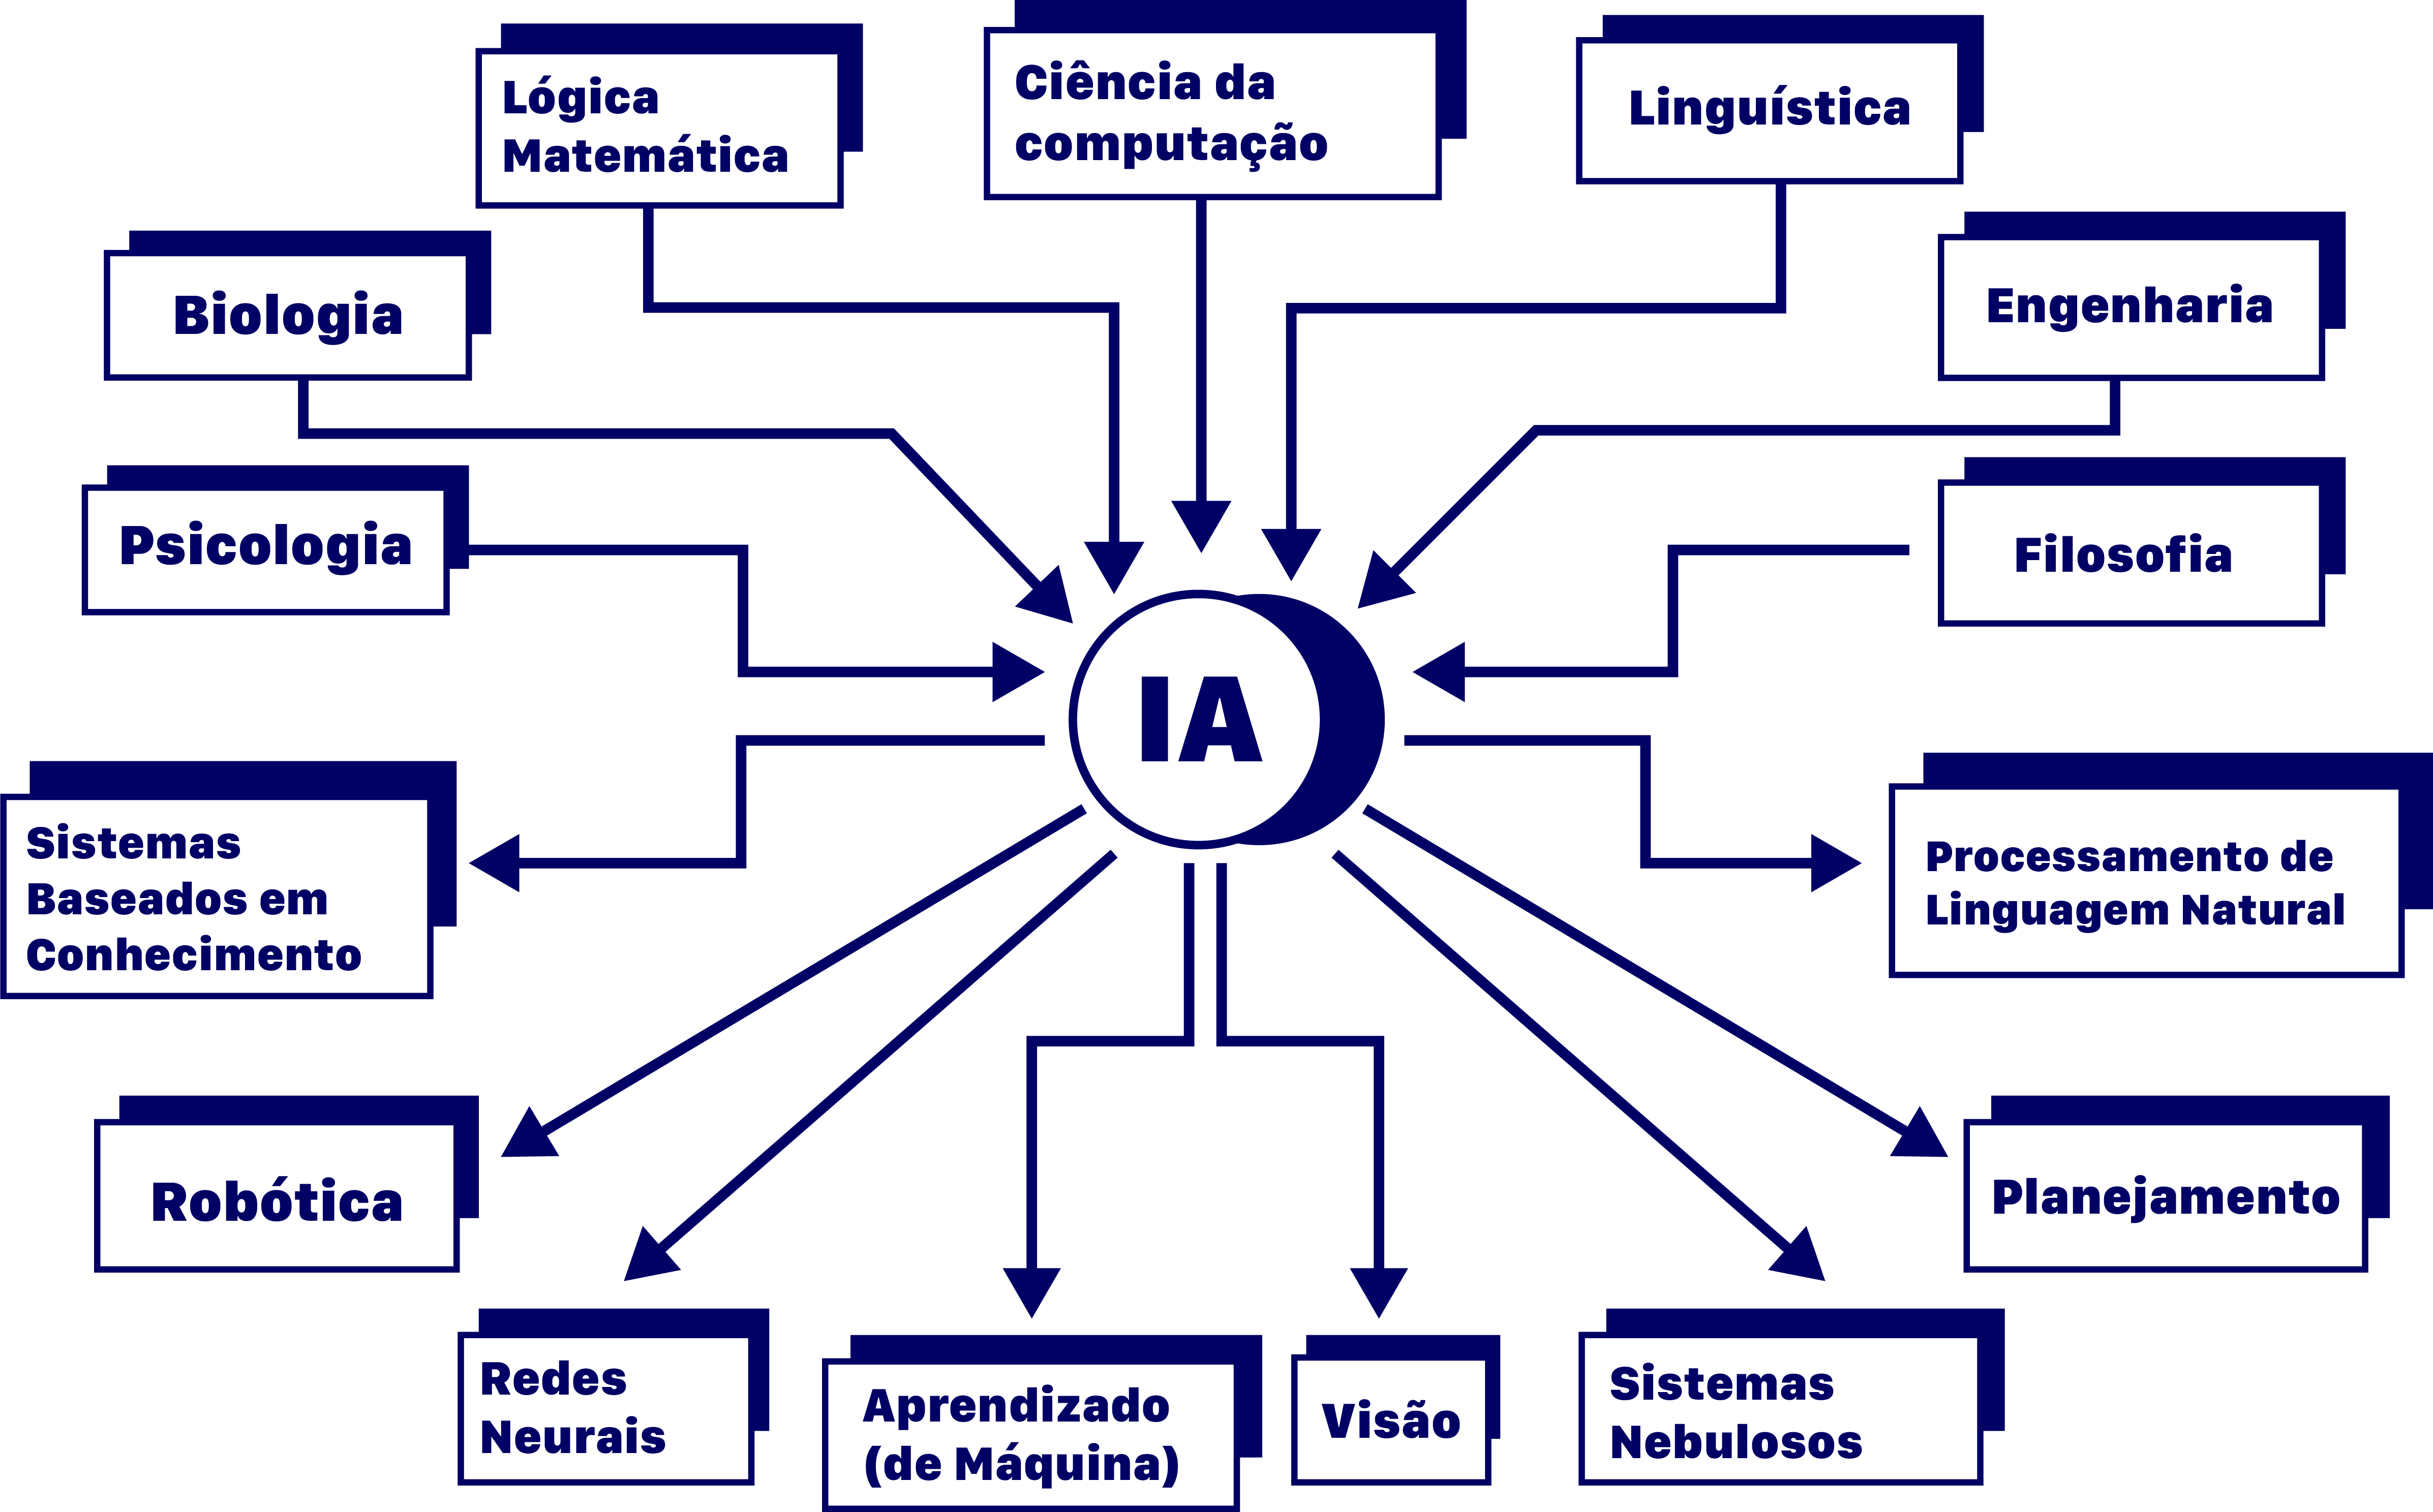
\includegraphics[width=10cm]{figures/areas_ia.png} % leia abaixo
	\legend{Fonte: \citeonline{aplicacoes_ia_vg}}
	\label{fig:areas_ia}
\end{figure}

Segundo \citeonline{dp_overview} existe três tópicos sobre inteligência artificial muito populares sendo eles, inteligência artificial, aprendizado de máquina e aprendizado profundo como segue na imagem \cref{fig:diagrama_ia_ml_dp}.

\begin{figure}[H]
	\caption{Diagrama de Venn sobre relação entre os tópicos de inteligência artificial}
	\centering % para centralizarmos a figura
	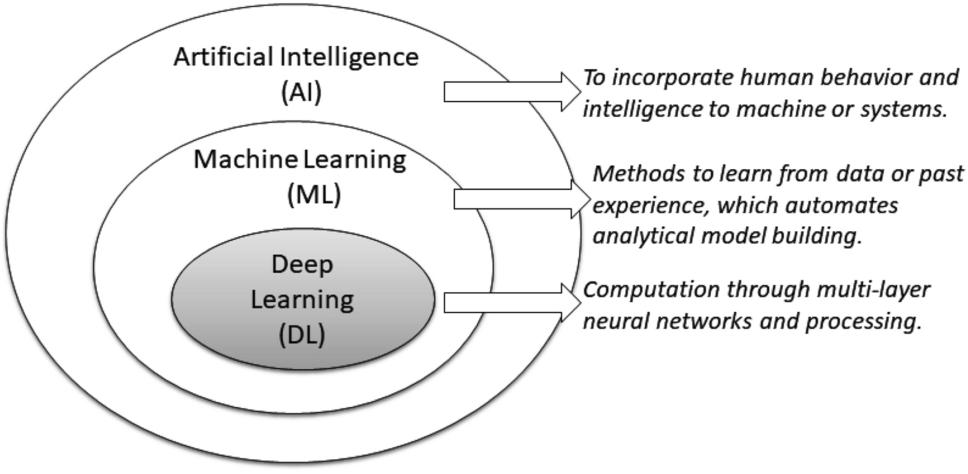
\includegraphics[width=10cm]{figures/diagrama_ia_ml_dp.png} % leia abaixo
	\legend{Fonte: \citeonline{dp_overview}}
	\label{fig:diagrama_ia_ml_dp}
\end{figure}



\subsection{Aprendizado de Máquina}

Segundo \citeonline{directions_ia_ml_dp}, aprendizado de máquina é uma subcategoria de inteligência artificial que se refere  a detecção de padrões importantes de uma base de dados. As ferramentas utilizadas aumentam a eficiência dos algoritmos para lidar com bases de dados grandes.

Portanto, essa técnica permite ao computador melhorar os resultados com base na experiência, isso indica uma relação direta entre o quanto o programa consumiu de dados e qualidade da solução do problema \cite{ml_explicado}. 

Dentro desse nicho existem outros como: redes neurais, algoritmos evolucionários, algoritmos de busca, aprendizado por reforço, dentre outros. \cite{ml_oil_gas_industry}.

É possível observar uma hierarquia entre aprendizado de máquina e os principais termos, sendo eles: redes neurais artificiais e aprendizado profundo com base em \citeonline{ml_and_dp} mostrado na ilustração da \cref{fig:diagrama_ann}. Esses termos são importantes para compreensão geral da área de segmentação contida em redes neurais.

\begin{figure}[H]
	\caption{Ilustração da relação entre os principais tópicos de aprendizado de máquina}
	\centering % para centralizarmos a figura
	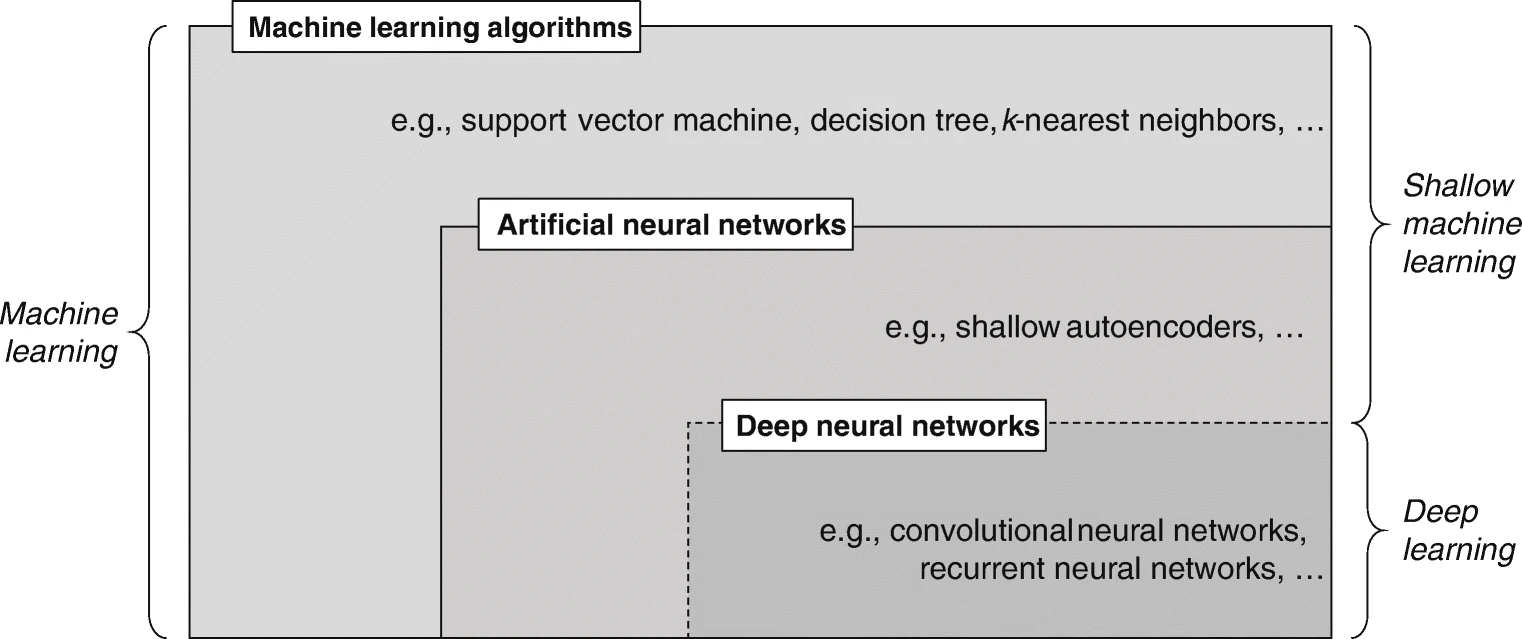
\includegraphics[width=10cm]{figures/diagrama_ann.jpg} % leia abaixo
	\legend{Fonte: \citeonline{ml_and_dp}}
	\label{fig:diagrama_ann}
\end{figure}


\subsubsection{Rede neural artificial}

Uma rede neural artificial é uma representação matemática de unidades de processamento conectadas chamadas de neurônios artificiais . Essa arquitetura simula sinapses, cada sinal trocado entre os neurônios pode aumentar ou atenuar os sinais de outros durante o aprendizado\cite{ml_and_dp}.
\begin{figure}[H]
	\centering
	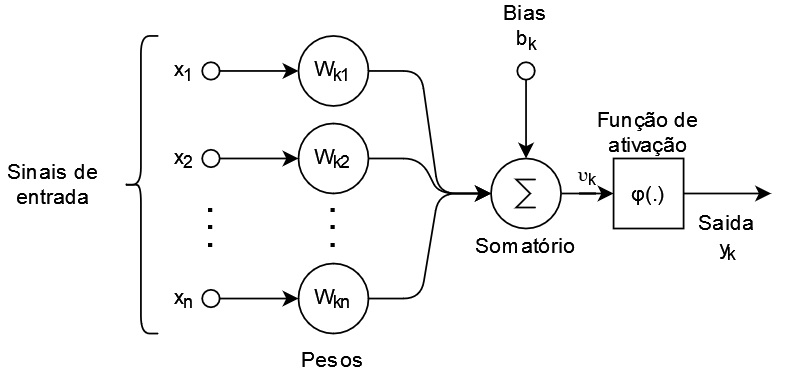
\includegraphics[width=0.8\textwidth]{figures/neuronio.png}
	\caption{Modelo de um neurônio não-linear \cite{haykin1999neural}.}
	\label{fig:neuronio}
\end{figure}

Observando a figura \ref{fig:neuronio} vemos o funcionamento de um neurônio $k$. Os sinais de entradas são partes de um vetor $x$ de tamanho $n$, sendo o vetor composto por $x_1, x_2 ... x_n$. Essas componentes são combinadas em uma soma ponderada utilizando seus respectivos pesos, $w_{k1}, w_{k2}...w_{kn}$, formando assim a seguinte equação  \apud{marti2017aprendizado}{haykin1999neural}:

$$\upsilon_k = \sum_{i=1}^n (x_i * w_{ki})$$

O resultado dessa equação produz o potencial de ativação $\upsilon_k$, esse resultado é somado com o \textit{bias} ou viés $b_k$ para manipular a saída $y_k$ do neurônio, essa soma é posta em uma função não-linear nomeada de função de ativação $\varphi(.)$, essas funções mapeiam a saída em um intervalo $[0, 1]$ ou $[1, -1]$. A função de saída pode ser representada com a seguinte equação \apud{marti2017aprendizado}{haykin1999neural}:

$$y_k = \varphi(\upsilon_k + b_k)$$

O aprendizado ocorre na fase de treinamento onde é ajustando os pesos $w_k$ e o viés $b_k$ de cada neurônio $k$. Os pesos $w_k$ são utilizados para calcular a taxa de crescimento da função e o viés $b_k$ é necessário para descolar a saída da função. Com isso é possível modelar uma função linear $y=w^T*x+b$ \cite{marti2017aprendizado}.

Para cada amostra o modelo compara os resultados dos valores atuais dos pesos $w_k$ e viés $b_k$ com o resultado esperado(alvo). Uma função custo(\textit{cost function}) é utilizada para gerar um vetor de gradientes e para quantificar o erro encontrado para a configuração atual do modelo. O modelo atualiza os pesos $w_k$ e os viés $b_k$ no sentido contrário do vetor de gradientes, buscando minimizar a função de custo de acordo com uma taxa de aprendizado(\textit{learning rate}) \cite{marti2017aprendizado}.

Ao combinar diversos neurônios artificiais forma-se uma rede neural Artificial. Essas redes buscam simular o processamento de informação do cérebro humano \cite{ferneda2006redes}.
Nas redes neurais os neurônios são organizados em grupos de unidade de processamento chamados camadas. A primeira e a última camada são nomeadas de camada de entrada e camada de saída e as demais de camadas ocultas. As camadas mais próximas da entrada são responsáveis por identificar características mais primitivas e as seguintes combinam essas informações para identificar padrões mais complexos \cite{marti2017aprendizado}.


\subsubsection*{Função de ativação}

A função de ativação retorna a saída de um neurônio \space\cite{haykin1999neural}, aqui pode-se ver quatro tipos de funções de ativação:

\begin{enumerate}
	\item Função \textit{Sigmoid}, uma função não-linear que produz uma curva com a forma de "S". Usada para mapear valores previstos em probabilidades. Tem o valor de saída entre 0 e 1 \space\cite{gharat2019what}.
	\begin{figure}[ht]
	\caption{Gráfico da função \textit{Sigmoid}.}
	\begin{center}
		\begin{minipage}{0.45\textwidth}
			\begin{equation}
				\varphi(\upsilon) = \frac{1}{1 + e^{-\upsilon}}
			\end{equation}
		\end{minipage}
		\hfill
		\begin{minipage}{0.45\textwidth}
			\begin{tikzpicture}
				\begin{axis}[
					width=0.9\textwidth,
					height=0.7\textwidth,
					xmin=-10, xmax=10,
					ymin=-0.2, ymax=1,
					xtick=\empty,
					ytick=\empty,
					axis lines=middle,
					xlabel={$\upsilon$},
					ylabel={$y$},
				]
					\addplot[blue,domain=-10:10,samples=51] {1/(1+exp(-x))};
				\end{axis}
			\end{tikzpicture}
		\end{minipage}
	\end{center}
	\legend{Fonte: Criação própria}
	\label{fig:grafico_sigmoid}
	\end{figure}
	Segundo \citeonline{gharat2019what}, a função \textit{Sigmoid} tem uma convergência lenta, é computacionalmente cara e para valores muito extremos causa problemas na previsão.

	\item Função \textit{ReLu} (Unidade Linear Retificada), função não-linear inspirada nos neurônios do cérebro que retorna um valor positivo ou 0 \space\cite{rizzo2020inteligencia}.
	\begin{figure}[ht]
	\caption{Gráfico da função \textit{ReLu}.}
	\begin{center}
		\begin{minipage}{0.45\textwidth}
			\begin{equation}
				\label{eq:relu_func}
				\varphi(\upsilon) = \max(0,\upsilon)
			\end{equation}
		\end{minipage}
		\hfill
		\begin{minipage}{0.45\textwidth}
			\begin{tikzpicture}
				\begin{axis}[
					width=0.9\textwidth,
					height=0.7\textwidth,
					xmin=-2, xmax=2,
					ymin=-0.5, ymax=2,
					xtick=\empty,
					ytick=\empty,
					axis lines=middle,
					xlabel={$\upsilon$},
        			ylabel={$y$},
				]
					\addplot[line width=1pt,color=blue,domain=-2:0] plot(\x,{0});
					\addplot[line width=1pt,color=blue,domain=0:2] plot(\x,{\x});
				\end{axis}
			\end{tikzpicture}
		\end{minipage}
	\end{center}
	\legend{Fonte: Criação própria}
	\label{fig:grafico_relu}
	\end{figure}
	A função \textit{ReLu} é computacionalmente eficiente e converge rapidamente, porém quando a entrada da função se aproxima de zero a rede neural não consegue executar o retropropagação, sendo assim não há aprendizado \space\cite{gharat2019what}.

	\item Função \textit{Leaky ReLU} (Unidade Linear Retificada com Vazamento), função não-linear variante da \textit{ReLU} que retorna um valor positivo ou $\upsilon/a_i$, sendo $a_i$ um valor na faixa $(1,\infty)$ \space\cite{xu2015empirical}.
	\begin{figure}[ht]
	\caption{Gráfico da função \textit{ReLu}.}
	\begin{center}
		\begin{minipage}{0.45\textwidth}
			\begin{gather}
				\label{eq:relu_leaky_func}
				\varphi(\upsilon) =
				\begin{cases}
				\upsilon & \text{if } \upsilon_k \geq 0 \\
				\frac{\upsilon}{a_k} & \text{if } \upsilon_k < 0
				\end{cases}
			\end{gather}
		\end{minipage}
		\hfill
		\begin{minipage}{0.45\textwidth}
			\begin{tikzpicture}
				\begin{axis}[
					width=0.9\textwidth,
					height=0.7\textwidth,
					xmin=-2, xmax=2,
					ymin=-0.5, ymax=2,
					xtick=\empty,
					ytick=\empty,
					axis lines=middle,
					xlabel={$\upsilon$},
        			ylabel={$y$},
				]
					\addplot[line width=1pt,color=blue,domain=-2:0] plot(\x,{0.3*\x});
					\addplot[line width=1pt,color=blue,domain=0:2] plot(\x,{\x});
				\end{axis}
			\end{tikzpicture}
		\end{minipage}
	\end{center}
	\legend{Fonte: Criação própria}
	\label{fig:grafico_relu_leaky}
	\end{figure}
	Possui as mesmas características da função \textit{ReLU}, mas sem o problema da retropropagação. \space\cite{gharat2019what}.

	\item Função \textit{Softmax}, calcula a distribuição de probabilidades de um evento em "n"\space eventos e fornece a probabilidade do valor de entrada pertencer a uma classe específica, geralmente usada na camada de saída \space\cite{gharat2019what}.
	\begin{figure}[ht]
	\caption{Gráfico da função \textit{Softmax}.}
	\begin{center}
		\begin{minipage}{0.45\textwidth}
			\begin{equation}
				\varphi(\upsilon) = \frac{e^{\upsilon_i}}{\sum_{j=0} e^{\upsilon_j}}
			\end{equation}
		\end{minipage}
		\hfill
		\begin{minipage}{0.45\textwidth}
			\begin{tikzpicture}
				\begin{axis}[
					width=0.9\textwidth,
					height=0.7\textwidth,
					xmin=-10, xmax=10,
					ymin=-0.2, ymax=1,
					xtick=\empty,
					ytick=\empty,
					axis lines=middle,
					xlabel={$\upsilon$},
        			ylabel={$y$},
				]
					\addplot[blue,domain=-10:10,samples=51] {exp(x)/sumexp(x,-4,0)};
				\end{axis}
			\end{tikzpicture}
		\end{minipage}
	\end{center}
	\legend{Fonte: Criação própria}
	\label{fig:grafico_softmax}
	\end{figure}
\end{enumerate}

Com a função \textit{Softmax} é possível normalizar a saída para valores entre 0 e 1, bem como calcular a probabilidade da entrada, e por causa dessas características é utilizada na camada de saída da rede neural \space\cite{gharat2019what}.


\subsubsection*{Função de perda}

A função de perda é calculada na camada de saída, e serve para mensurar o sucesso obtido comparando com fórmulas o resultado predito com o resultado real do conjunto de dados. O resultado dessa função irá ajudar na retropropagação, \emph{i.e.}, servirá para ajustar os pesos e vieses da conexão entre os neurônios para minimizar o erro. A seguir algumas funções de perda, pontuando que todo esse subtópico é baseado em 
\citeonline{Alzubaidi2021}.

\subsubsubsection*{Softmax ou entropia cruzada ou logarítmica}

Muito utilizada para medir a performance de uma rede neural convolucional principalmente quando o resultado tem várias classes. Antes dessa função de perda é necessário usar a função de ativação softmax descrita na \cref{fig:grafico_softmax}, pois precisa de uma saída dentro de uma distribuição de probabilidade. Sendo N o número de classes ou o número de neurônios na camada de saída.

\begin{equation} 
    H(p,y) = -\sum_{i=1}^N y_i \log(p_i)
\end{equation}


\subsubsubsection*{Euclidiana ou erro quadrático médio}

Muito utilizada para problemas de regressão.

\begin{equation}
    H(p,y) = \frac{1}{2N} \sum_{i=1}^N (p_i - y_i)^2
\end{equation}

\subsubsubsection*{Hinge}

Muito utilizado para classificação binária.

\begin{equation}
    H(p,y) = \sum_{i=1}^N max(0, m - (2y_i - 1) p_i)
\end{equation}


% \subsubsection*{Retropropagação}

De acordo com \space\citeonline{brilliant2023backpropagation} o algoritmo geral de retropropagação é:

\begin{enumerate}
    \item Propagação: calcular os pares de entrada-saída $(\overrightarrow{x_d}, y_d)$ — $\overrightarrow{x_d}$ é o vetor de entrada e $y_d$ a saída verdadeira — e guardar os resultados $\hat{y_d}$ — a saída encontrada no treinamento —, $a_j^k$, $o_j^k$ para cada neurônio $j$ na camada $k$, indo da camada de entrada para camada de saída.
    
    \item Retropropagação: Calcular os pares de entrada-saída $(\overrightarrow{x_d}, y_d)$, chegando na fórmula $\frac{\partial{E_d}}{\partial{w_{ij}^k}}$ que é a derivada parcial do erro total. Na representação $E_d$ é a função de perda e $w_{ij}^k$ é o peso  conectado em um neurônio de $k - 1$. Outra forma de representar é $\delta_j^k o_i^{k - 1}$ e suas variáveis são: $\delta_j^k$ representa o erro do neurônio e $o_i^{k - 1}$ representa a saída do neurônio na camada $k -1$. Essa técnica começa na camada de saída e propaga até a última camada escondida.
    
    \begin{equation}
        \frac{\partial{E_d}}{\partial{w_{ij}^k}} = \delta_j^k o_i^{k - 1} 
    \end{equation}
    
    \item Combinar gradientes individuais: Uma média simples é feita com todos resultados de $\frac{\partial{E_d}}{\partial{w_{ij}^k}}$ formando assim o gradiente total representado como $\frac{\partial{E(X, \theta)}}{\partial{w_{ij}^k}}$.
    
    \begin{equation}
        \frac{\partial{E(X,\theta)}}{\partial{w_{ij}^k}} = \frac{1}{N} \sum_{d=1}^{N} \frac{\partial{E_d}}{\partial{w_{ij}^k}}
    \end{equation}
    
    \item Atualiza os pesos: usando $\alpha$ como taxa de aprendizado e o gradiente total $\frac{\partial{E(X, \theta)}}{\partial{w_{ij}^k}}$ tem-se a seguinte equação.
    
    \begin{equation}
        \Delta w_{ij}^k = -\alpha \frac{\partial{E(X,\theta)}}{\partial{w_{ij}^k}}
    \end{equation}
\end{enumerate}

Observação: basta trocar $w_{ij}^k$ para $b_{ij}^k$ — trocar o peso pelo viés — em todo algoritmo para ajustar o viés do modelo com a técnica de retropropagação.


\subsubsection*{Regularização}

Quando se monta uma arquitetura de redes neurais convolucional pode se chegar em três casos sendo eles: sobreajuste (overfit), subajuste (underfit) e balanceado (optimal). O sobreajuste é quando no treinamento o modelo acerta as classes porém nos testes não, isso mostra uma dificuldade em generalizar as características. Já o subajuste não consegue pontuar bem em nenhum caso mostrando que o conjunto de dados de treinamento está pequeno para detectar padrões. Por outro lado o balanceado é quando produz resultados bons tanto no conjunto de dados de treinamento quanto no de testes \cite{Alzubaidi2021, computation11030052}.

\begin{figure}[H]
	\caption{Gráficos mostrando subajuste, balanceado e sobreajuste respectivamente}
	\centering % para centralizarmos a figura
	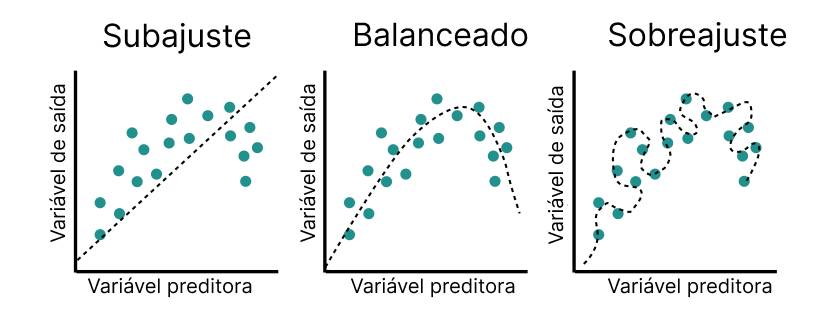
\includegraphics[width=15cm]{figures/fittings.png} % leia abaixo
	\legend{Fonte: \citeonline{educative2022overfitting}}
	\label{fig:arquitetura_cnn}
\end{figure}

\subsubsection*{Rede neural profunda}

A principal diferença entre uma rede neural artificial e uma rede neural profunda é a quantidade de camadas, uma rede neural profunda possui várias camadas de processamento \apud{marti2017aprendizado}{haykin1999neural}.

\begin{figure}[ht]
	\centering
	\caption{Comparação de uma rede neural convencional com uma rede neural profunda.}
	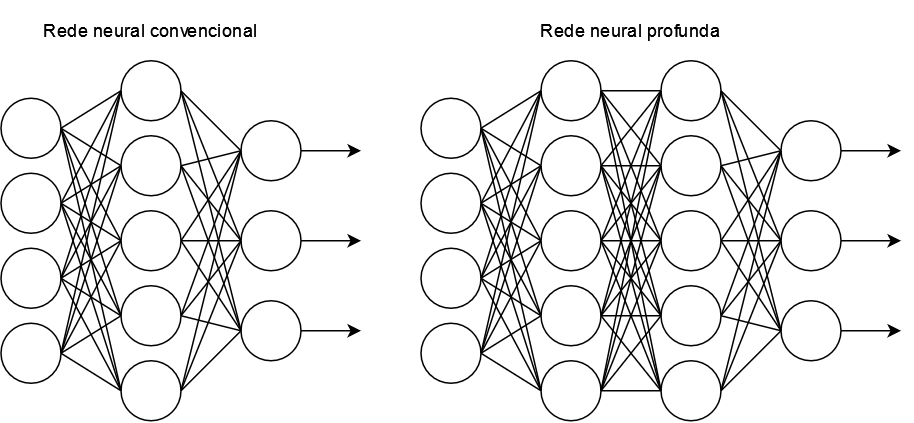
\includegraphics[width=0.8\textwidth]{figures/redes_neurais.png}
	\legend{Fonte: Criação própria}
	\label{fig:redes_neurais}
\end{figure}

% \subsection{Aprendizado profundo}

O aprendizado profundo é uma área do aprendizado de máquina caracterizada por utilizar dados brutos como entrada e descobrir as representações necessárias para permitir o mapeamento adequado e assim tornando as soluções mais simples \apud{marti2017aprendizado}{lecun2015deep}.

Segundo \space\citeonline{lecun2015deep}, o aprendizado profundo são métodos de representação de aprendizado com vários níveis, obtidos por meio da decomposição de módulos simples e lineares, que transformam a representação de um nível em uma representação mais alta e abstrata. Por exemplo a representação de uma imagem é transformada em informações que identificam objetos.

Dividindo um problema complexo em problemas menores torna os métodos especializados, viabilizando tarefas mais complexas, depois essas tarefas que foram dividias são recombinadas e é gerado uma solução do problema \space\cite{marti2017aprendizado}.

Utilizando o exemplo anterior, reconhecimento de imagem, cada um desses métodos especializados seria responsável por reconhecer uma parte da imagem, como bordas, objetos, tamanho, etc. E após a junção desses métodos é feito a predição da imagem \space\cite{marti2017aprendizado}.

A principal diferença entre uma rede neural convencional e uma rede neural profunda é a quantidade de camadas, uma rede neural profunda possui várias camadas de processamento \apud{marti2017aprendizado}{haykin1999neural}.

\begin{figure}[ht]
	\centering
	\caption{Comparação de uma rede neural convencional com uma rede neural profunda.}
	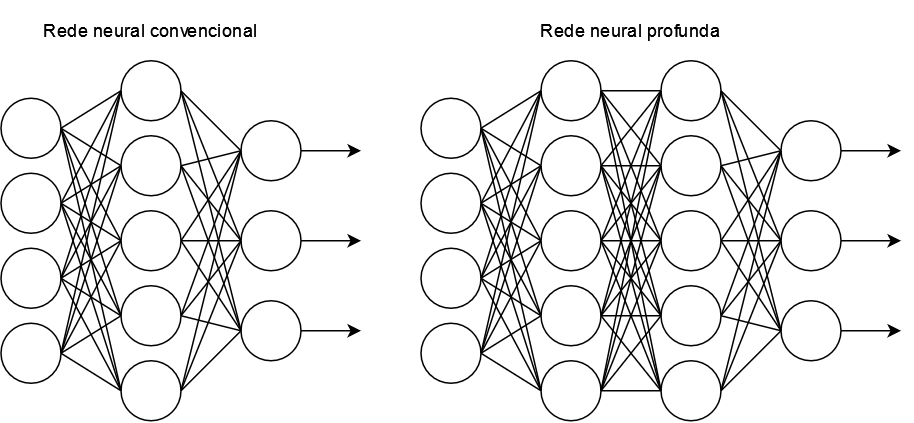
\includegraphics[width=0.8\textwidth]{figures/redes_neurais.png}
	\legend{Fonte: Criação própria}
	\label{fig:redes_neurais}
\end{figure}


\subsubsubsection{Redes neurais convolucionais}

Uma rede neural convolucional é análoga à rede neural artificial, i.e., feita de neurônios que otimizam o aprendizado através dele mesmo. A principal diferença é que a rede neural convolucional é amplamente utilizada em soluções que detectam padrões em imagens, logo existem funcionalidades específicas da própria arquitetura para essa tarefa \cite{oshea2015introduction}. 

Uma arquitetura básica de uma rede neural convolucional tem as seguintes camadas: convolucional, agrupamento e totalmente conectada. Ilustrada na \cref{fig:arquitetura_cnn} \cite{dp_overview}.

\begin{figure}[ht]
	\caption{Camadas principais de uma rede neural convolucional}
	\centering % para centralizarmos a figura
	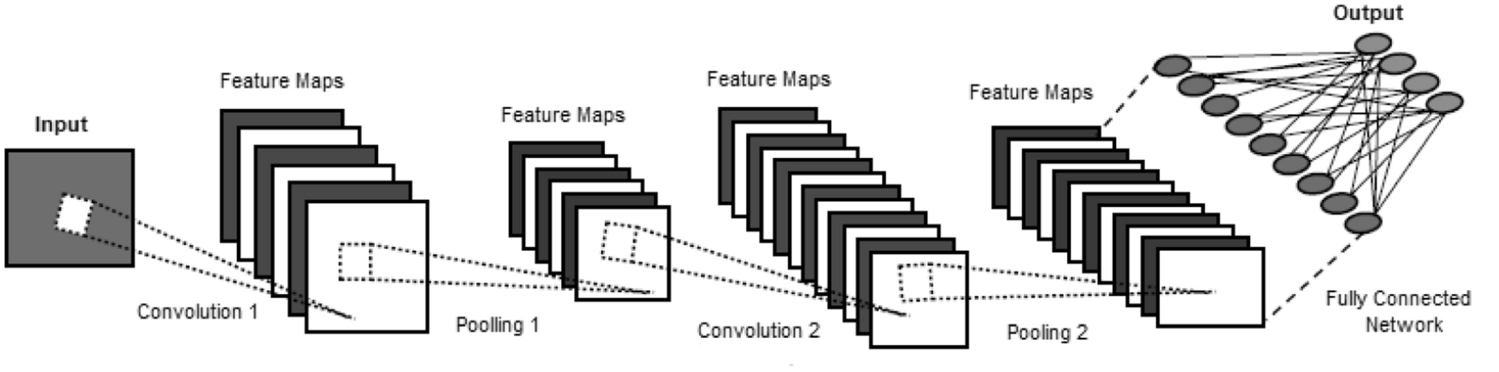
\includegraphics[width=15cm]{figures/arquitetura_cnn.png} % leia abaixo
	\legend{Fonte: \citeonline{dp_overview}}
	\label{fig:arquitetura_cnn}
\end{figure}

\subsubsubsection*{Camada convolucional}

Segundo \citeonline{computation11030052} camada convolucional é essencial para esse tipo de arquitetura e usa um filtro — ou kernel — para aplicar na imagem e direcionar para o próximo neurônio. Esse filtro é uma matriz de números que terá uma operação aplicada em todos os píxeis da imagem — que também é representado por matriz(es) — as informações cruciais para esse filtro são: tamanho, largura e pesos. Isto é utilizado para extrair características com uma base matemática, criando uma relação direta entre um píxel e os píxeis ao redor. Os pesos começam de forma pseudoaleatórias e são ajustados no decorrer do aprendizado. O resultado dessa camada é chamado de mapa de características. O tamanho da saída será baseado na fórmula abaixo sendo os tamanhos I da imagem, F do filtro e a S da saída \cite{computation11030052}.

\begin{gather}
    \mathbf{I}x - \mathbf{F}x + 1 = \mathbf{S}x \notag \\
    \mathbf{I}y - \mathbf{F}y + 1 = \mathbf{S}y
\end{gather}

    
A seguir um exemplo dos passos para construir a matriz resultante baseado em \citeonline{Alzubaidi2021}.

\clearpage

$$
\hspace{0.4cm}
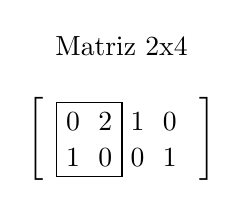
\begin{tikzpicture}[baseline=(M.center)]
 \matrix (M) [matrix of math nodes,left delimiter={[},right delimiter={]}] {
 0 & 2 & 1 & 0 \\
 1 & 0 & 0 & 1 \\
 };
 \draw (M-1-1.north west) rectangle (M-2-2.south east);
 \node[above=10pt of M.north] {Matriz 2x4};
\end{tikzpicture}
\hspace{0.8cm}\bigotimes\hspace{0.8cm}
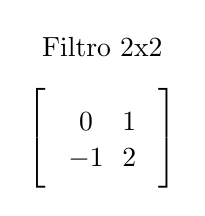
\begin{tikzpicture}[baseline=(M.center)]
 \matrix (M) [matrix of math nodes,left delimiter={[},right delimiter={]}] {
  0 & 1 \\
 -1 & 2 \\
 };
 \node[above=10pt of M.north] {Filtro 2x2};
\end{tikzpicture}
\hspace{0.8cm}=\hspace{0.8cm}
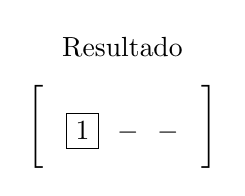
\begin{tikzpicture}[baseline=(M.center)]
 \matrix (M) [matrix of math nodes,left delimiter={[},right delimiter={]}] {
    \boxed{1} & - & - \\
 };
 \node[above=10pt of M.north] {Resultado};
\end{tikzpicture}
$$

$$
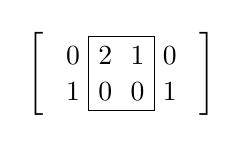
\begin{tikzpicture}[baseline=(M.center)]
 \matrix (M) [matrix of math nodes,left delimiter={[},right delimiter={]}] {
    0 & 2 & 1 & 0 \\
    1 & 0 & 0 & 1 \\
 };
 \draw (M-1-2.north west) rectangle (M-2-3.south east);
\end{tikzpicture}
\hspace{0.8cm}\bigotimes\hspace{0.8cm}
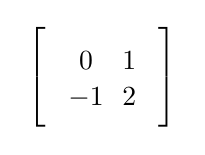
\begin{tikzpicture}[baseline=(M.center)]
 \matrix (M) [matrix of math nodes,left delimiter={[},right delimiter={]}] {
  0 & 1 \\
  -1 & 2 \\
 };
\end{tikzpicture}
\hspace{0.8cm}=\hspace{0.8cm}
\begin{bmatrix}
 1 & \boxed{1} & - \\
 \end{bmatrix}
$$

$$
\hspace{0.2cm}
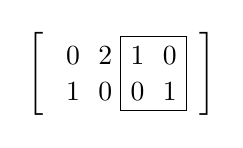
\begin{tikzpicture}[baseline=(M.center)]
 \matrix (M) [matrix of math nodes,left delimiter={[},right delimiter={]}] {
    0 & 2 & 1 & 0 \\
    1 & 0 & 0 & 1 \\
 };
 \draw (M-1-3.north west) rectangle (M-2-4.south east);
\end{tikzpicture}
\hspace{1cm}\bigotimes\hspace{0.9cm}
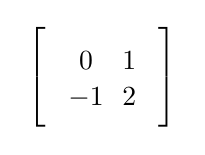
\begin{tikzpicture}[baseline=(M.center)]
 \matrix (M) [matrix of math nodes,left delimiter={[},right delimiter={]}] {
  0 & 1 \\
  -1 & 2 \\
 };
\end{tikzpicture}
\hspace{0.8cm}=\hspace{0.8cm}
\begin{bmatrix}
 1 & 1 &  \boxed{2} \\
 \end{bmatrix}
$$

\subsubsubsection*{Tamanho do passo e preenchimento}

O tamanho do passo — ou stride — serve para especificar a distância de pixels entre os passos da camada.  No exemplo acima esse parâmetro é definido como 1, por isso a matriz selecionada pula 1 pixel para direita entre os passos. Esse valor altera o tamanho da matriz resultante \cite{dp_overview}.

O preenchimento — ou padding — é uma técnica utilizada para manter o mesmo tamanho da entrada, adicionando bordas com zeros antes das operações da camada para ter como saída uma matriz da mesma dimensão da matriz original. Isso é usado devido a desvantagem em perder os detalhes nas bordas das imagens no processamento de uma camada \cite{dp_overview}.

\subsubsubsection*{Camada de agrupamento}

A camada de agrupamento — ou pooling — tem como tarefa primordial uma técnica para reduzir o tamanho do mapa de características, porém preservando os padrões mais relevantes. Dentre os recursos essenciais dessa camada estão o tamanho do agrupamento e a operação que será realizada. O maior problema dessa camada é pelo fato dela apenas identificar onde essas características estão e não se tem ou não, \emph{i.e.}, dependendo de qual operação e a quantidade de camadas pode não ser possível guardar as principais características de forma integra causando uma redução no desempenho final da predição \cite{dp_overview}.

Existem vários tipos de agrupamento, os mais utilizados são: agrupamento máximo, agrupamento médio e agrupamento global médio que estão explicados abaixo em exemplos baseados em \citeonline{Alzubaidi2021}.

\subsubsubsection*{Agrupamento máximo}

É definido o resultado com base no máximo encontrado pelo tamanho do agrupamento, exemplo a seguir usando um mapa de características com tamanho 4x4 e agrupamento de tamanho 2x2.

$$
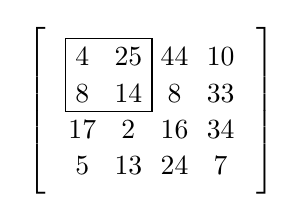
\begin{tikzpicture}[baseline=-0.5ex]
    \matrix (M) [matrix of math nodes,left delimiter={[},right delimiter={]}] {
        4 & 25 & 44 & 10\\
        8 & 14 & 8 & 33 \\
        17 & 2 & 16 & 34 \\
        5 & 13 & 24 & 7 \\
    };
    \draw (M-1-1.north west) rectangle (M-2-2.south east);
\end{tikzpicture}
= 
\begin{bmatrix}
	\boxed{25} & 44 \\
	17 & 34 \\
   \end{bmatrix}
$$

\subsubsubsection*{Agrupamento médio}

É definido o resultado com base na média encontrada pelo tamanho do agrupamento, exemplo a seguir usando um mapa de características com tamanho 4x4 e agrupamento de tamanho 2x2.

$$
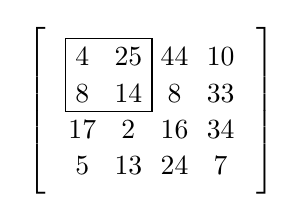
\begin{tikzpicture}[baseline=-0.5ex]
    \matrix (M) [matrix of math nodes,left delimiter={[},right delimiter={]}] {
        4 & 25 & 44 & 10\\
        8 & 14 & 8 & 33 \\
        17 & 2 & 16 & 34 \\
        5 & 13 & 24 & 7 \\
    };
    \draw (M-1-1.north west) rectangle (M-2-2.south east);
\end{tikzpicture}
= 
\begin{bmatrix}
	\boxed{12} & 23 \\
	9 & 20 \\
   \end{bmatrix}
$$

\subsubsubsection*{Agrupamento global médio}

É definido o resultado com base na média geral do mapa o que sempre tem como saída uma matrix 1x1, exemplo a seguir usando um mapa de características com tamanho 4x4.

$$
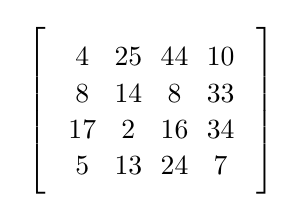
\begin{tikzpicture}[baseline=-0.5ex]
    \matrix (M) [matrix of math nodes,left delimiter={[},right delimiter={]}] {
        4 & 25 & 44 & 10\\
        8 & 14 & 8 & 33 \\
        17 & 2 & 16 & 34 \\
        5 & 13 & 24 & 7 \\
    };
\end{tikzpicture}
= 
\begin{bmatrix}
	16
   \end{bmatrix}
$$

\subsubsubsection*{Camada totalmente conectada}

A camada totalmente conectada geralmente é utilizada no final da arquitetura e cria a partir de cada neurônio uma ligação direta para cada etiqueta final. Isso torna essa camada extremamente pesada computacionalmente. O número de neurônios dessa camada é equivalente ao número de classes propostas. Além disso é quando chega nessa camada que a função de perda é calculada e se inicia a retropropagação \cite{Alzubaidi2021, computation11030052}.

\subsubsubsection*{Aperfeiçoamento}

Segundo \citeonline{Alzubaidi2021, computation11030052} existem algumas técnicas para aperfeiçoar os resultados do modelo, sendo elas:

\begin{itemize}
    \item Dropout: Muito utilizada para evitar sobreajuste pois está técnica irá desligar um neurônio aleatoriamente colocando a saída dele como zero no processo de treinamento e portanto forçara o modelo a aprender a identificar características diferentes em outros neurônios possibilitando a generalização do modelo.
    \item Aumentar o tamanho do conjunto de dados: caso não seja possível criar ou encontrar um maior existem técnicas para aumentar artificialmente acrescentando pequenas mudanças nas imagens existentes, algumas são rotacionar, recortar e inverter horizontalmente ou verticalmente.
    \item Normalização em lote: normaliza as saídas para treinar a rede mais rápido
    \item Aumentar o tempo de treinamento
    \item Aumentar a profundidade ou largura da arquitetura
    \item Ajustar os hiperparâmetros
\end{itemize}
    

\subsection{Segmentação}



\subsubsubsection*{EfficientPS}
\label{sec:EfficientPS}

EfficientPS é uma solução para a segmentação panóptica proposta no artigo \citeonline{mohan2020efficientps}, o trabalho apresenta uma arquitetura que se inicia com um backbone — parte para identificar características — usando uma Rede de Pirâmide de Características(RPC)\footnote{Estrutura de pirâmide para extrair características em várias escalas de uma imagem \space\cite{piramide}} de 2 caminhos seguido de dois cabeçotes paralelos um para uma arquitetura de segmentação semântica que é autoria deles e outra de instância com modificações baseadas na topologia Mask R-CNN e finalmente a saída dos dois cabeçotes são combinadas no módulo de fusão panóptica para gerar a saída final com a imagem de segmentação panóptica, esta arquitetura é ilustrada na \cref{fig:arqEP}.

\begin{figure}[ht]
	\caption{Arquitetura geral do EfficientPS}
	\centering % para centralizarmos a figura
	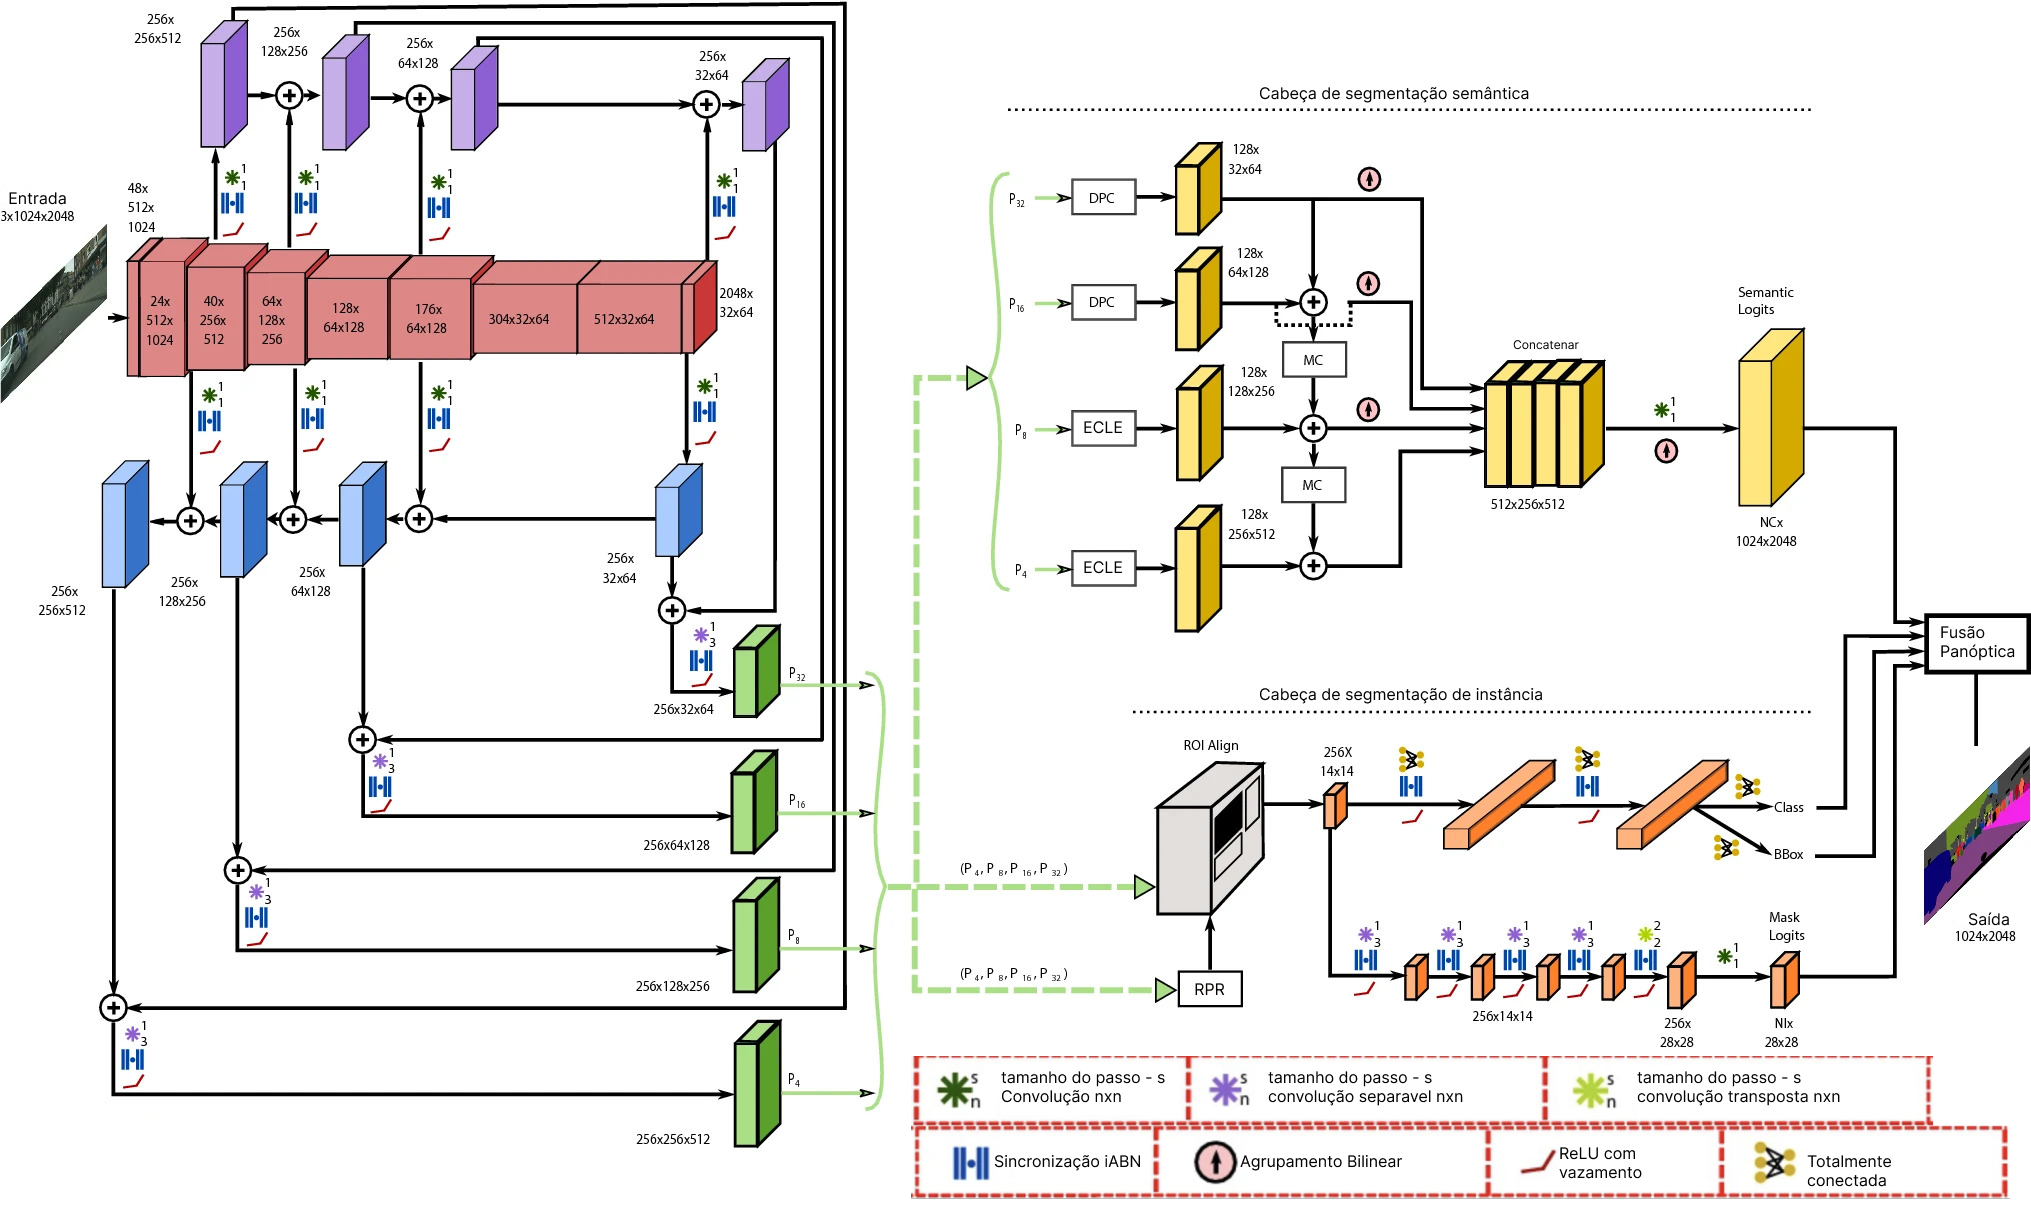
\includegraphics[width=15cm]{figures/arqEP.png} % leia abaixo
	\legend{Fonte: \citeonline{mohan2020efficientps}}
	\label{fig:arqEP}
\end{figure}

\subsubsubsection*{Backbone da rede}

A espinha dorsal — ou backbone — se consiste em uma codificação combinado a uma bifurcação paralela usando RPC. O codificador é essencial para arquiteturas de segmentação e para melhorar a capacidade de representação é necessário aumentar o número de parâmetros e a complexidade, porém nesse artigo os autores chegaram numa solução balanceada nesse quesito. O codificador contém nove blocos (em vermelho), mostrado na \cref{fig:arqEP} e a 2º, 3º, 5º e 9º saídas — da esquerda para diretira — correspondem aos fatores de redução de amostragem x4,x8,x16 e x32 respectivamente. Essas saídas vão conectar com a bifurcação paralela que são de sentidos opostos para gerar mais detecções de características. Após isso será feita uma combinação entre camadas de mesma dimensão utilizando camadas de convolução separável em profundidade — divide em etapa espacial e de canal, aplicada a cada canal e cada pixel de saída respectivamente — resultando nas saídas $ P_4 + P_8 + P_{16} + P_{32} $\cite{mohan2020efficientps, redes-neurais-convolucionais-separaveis-em-profundidade}.

\subsubsubsection*{Cabeçote de Segmentação Semântica}

O cabeçote de segmentação semântica é autoria dos autores e é dividido em três módulos sendo eles: Extrator de Características em Larga Escala (ECLE) — ou Large Scale Feature Extractor (LSFE) — para capturar recursos finos em larga escala de forma eficiente, módulo DPC deve ser capaz de capturar contexto de longo alcance, porém em pequena escala e o módulo MC deve ser capaz de mitigar a incompatibilidade entre recursos de grande e pequena escala nas camadas de agregação \space\cite{mohan2020efficientps}.

As quatro entradas do cabeçote $ P_4 + P_8 + P_{16} + P_{32} $ são separadas, sendo $ P_{16} + P_{32} $ — pequena escala — alimentam dois módulos DPC paralelos e $ P_4 + P_8 $ — larga escala — alimentam dois módulos ECLE paralelos \space\cite{mohan2020efficientps}.

\subsubsubsection*{Cabeçote de segmentação de instância}

Este cabeçote é derivada da arquitetura Mask R-CNN e as modificações foram três, sendo: trocar a convolução padrão por convolução separável em profundidade — para reduzir o número de parâmetros consumidos pela rede —, camada de normalização em lote foi substituída por iABN Sync\footnote{normalização em lotes entre cores de GPU para aumentar o desempenho} e a função ReLU definida em \cref{eq:relu_func} por Leaky ReLU definida em \cref{eq:relu_leaky_func} \space\cite{mohan2020efficientps,redes-neurais-convolucionais-separaveis-em-profundidade, serp-ai}.

\subsubsubsection*{Módulo de fusão panóptica}

O módulo da fusão panóptica é necessário para construir a imagem com segmentação panóptica. Nessa parte os resultados são unidos aos dois cabeçotes anteriormente explicados. Esta tarefa não é simples pois é necessário criar uma lógica para obter o melhor resultado diante das sobreposições encontradas. O módulo foi criado no intuito de ser adaptativo e usar as duas entradas de forma equivalente \space\cite{mohan2020efficientps}.

Resumindo o módulo aplica algumas técnicas para reduzir o número de instâncias baseando-se na métrica logist — valor numérico que pontua confiança — aplica algumas agregações entre os resultados dos dois cabeçotes e desenha com fundo preto as instâncias com melhor classificação de confiança, logo depois preenche com a parte de stuff — classes semânticas sem importância — da entrada semântica \space\cite{mohan2020efficientps}.

\section{Trabalhos relacionados}

Esta seção destina-se a análise e discussão da metodologia e dos resultados prospostos por \citeonline{geracao_procedural_jogos_2d,kirillov2019panoptic}. 

\subsection*{Geração Procedural de Mapas para Jogos 2D}

No trabalho \citeonline{geracao_procedural_jogos_2d}, é apresentado uma solução simples para criar mapas de cavernas, calabouços e ilhas para jogos 2D. O algoritmo foi dividido em três partes sendo elas: geração recursiva de terrenos, validação de tamanho e correção da coesão. Os autores concluíram que não existe literatura sobre geração procedural de salas diversas e corredores distintos como o algoritmo proposto. Sugerem duas possibilidades para trabalhos futuros sendo elas: usar algoritmos genéticos para mensurar a qualidade dos mapas gerados e promover pela seleção natural e a outra possibilidade é mesclar o algoritmo proposto com técnicas de geração de salas interligadas por corredores, de forma a possibilitar a criação de mapas com algumas salas pré-definidas inseridas em um mapa aberto contínuo.

\subsection*{Panoptic Segmentation}

No trabalho \citeonline{kirillov2019panoptic} é definido a ideia geral de segmentação panóptica além de definir conceitos importantes como coisas e objetos e a métrica unificada para medir o desempenho de modelos dessa área. Também é feito alguns testes comparando resultados humanos com um modelo simples proposto com eles combinando PSPNet e Mask R-CNN usando a métrica de qualidade panóptica definida por eles. Os resultados mostraram a superioridade humana na segmentação panóptica em três conjuntos de dados diferentes, sendo eles: Cityscapes, ADE20k e Vistas, as métricas usadas foram qualidade panóptica, qualidade semântica, qualidade de reconhecimento, qualidade panóptica
 de coisas e qualidade panóptica de objetos. O melhor resultado para a máquina em comparação com o humano foi no conjunto de dados Cityscapes avaliando a qualidade semântica, sendo 84,1 para o humano e 80,9 para máquina. O pior resultado para a máquina em relação ao humano foi no conjunto de dados ADE20k na qualidade panóptica de coisas, sendo 71,0 para os humanos e 24,5 para a máquina.

 \subsection*{}

\chapter{Desenvolvimento}

Neste capítulo é apresentada a descrição da proposta e relatado o processo de
desenvolvimento e avaliação da implementação.

\section{Proposta}

Este trabalho tem como proposta a utilização de um modelo de inteligência artificial para segmentação panóptica que irá classificar os pixeis na imagem e permitir que os usuários gerem mapas procedurais a partir da seleção de um dos segmentos da imagem.

Utilizando o modelo EfficientPS é possível fazer a segmentação panóptica, segue exemplos nas \crefrange{fig:segmantations_1}{fig:segmantations_2}. O modelo citado está disponível no GitHub dos próprios autores \citeonline{mohan2020efficientps}
% e será treinado com a combinação de pelo menos dois conjuntos de dados citados anteriormente.
 No resultado apenas será identificado os pixeis de classes contidas nos conjuntos de dados escolhidos, portanto é possível que em uma imagem não seja identificado nada:

\begin{figure}[!ht]
	\centering
    \caption{Imagem de entrada para rede neural.}
	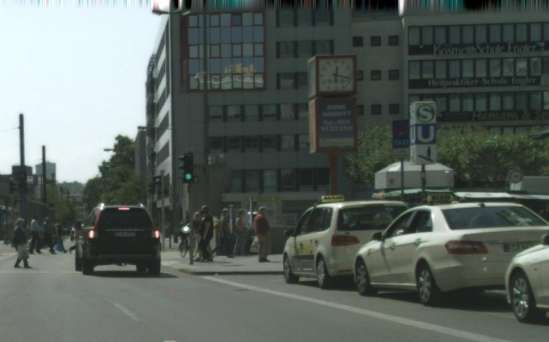
\includegraphics[width=0.6\textwidth]{figures/segmantations_1.png}
    \legend{Fonte: \citeonline{kirillov2019panoptic}}
	\label{fig:segmantations_1}
\end{figure}

\begin{figure}[!ht]
	\centering
    \caption{Imagem saída de um modelo de segmentação panóptica de segmentação panóptica.}
	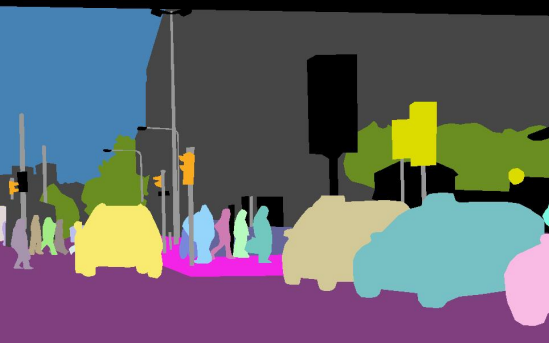
\includegraphics[width=0.6\textwidth]{figures/segmantations_2.png}
    \legend{Fonte: \citeonline{kirillov2019panoptic}}
	\label{fig:segmantations_2}
\end{figure}

Após a segmentação da imagem o usuário poderá selecionar qual parte da imagem será utilizada para gerar a ilha.

Feito a seleção será gerado um diagrama de Voronoi que funcionará como um filtro em cima dessa imagem, assim gerando a ilha e os biomas.

\begin{figure}[!ht]
	\centering
    \caption{Ilha gerada a partir da segmentação panóptica e aplicando um filtro com o diagrama de Voronoi, azul representa oceano, verde floresta, cinza montanhas.}
	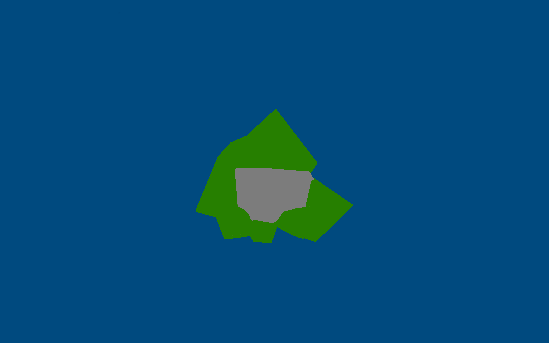
\includegraphics[width=0.6\textwidth]{figures/segmantations_pnl.png}
    \legend{Fonte: Criação própria}
	\label{fig:segmantations_pnl}
\end{figure}



\section{Implementação}

Pode-se dividir a implementação em cinco partes, sendo elas: segmentar imagens, selecionar contorno, gerar proceduralmente o mapa com biomas, analisar casos de pós processamento e interligar as ferramentas atráves de uma interface gráfica.

\subsection{Segmentar imagens}

A segmentação da imagem é usada para classificar os pixels da imagem a partir de padrões reconhecidos por uma inteligência artificial. A partir disso é possível o usuário selecionar o contorno para gerar o mapa.

A linguagem de programação utilizada para desenvolvimento do projeto foi Python pois existem muitas bibliotecas que auxiliam na criação de arquiteturas complexas de Inteligência Artificial como o \hyperref[sec:EfficientPS]{EfficientPS}.

Utilizou-se o código aberto oficial do trabalho ciéntifico postado no repositório do Github \footnote{\url{https://github.com/DeepSceneSeg/EfficientPS}} que foi baseado no tópico \hyperref[sec:EfficientPS]{EfficientPS}.

Utilizou-se um arquivo pré treinado desse modelo contendo o aprendizado do conjunto de imagens do \textit{Cityscapes} para segmentação panóptica, a ideia inicial era treinar com pelo menos mais um conjunto de dados porém surgiu-se diversos desafios para serem solucionados, dentre eles: conseguir autorização para baixar conjuntos de dados específicos para segmentação panóptica, outro problema foi preparar esse conjunto de dados para processar o aprendizado, além de problemas de limitação de processamento bruto. Portante decidiu-se utilizar o próprio modelo salvo baixado do repositório.

Percebeu-se que o resultado do modelo proposto não foi o esperado pois objetos de mesma classe como carros tem a mesma cor com uma borda branca exemplificados na \cref{fig:resultado_inicial}. Logo tentou-se mudar o código para gerar uma saída com objetos de mesma classe com cores diferentes como na figura \cref{fig:segmantations_2}.

\begin{figure}[!ht]
	\centering
    \caption{Resultado inicial do repositório.}
	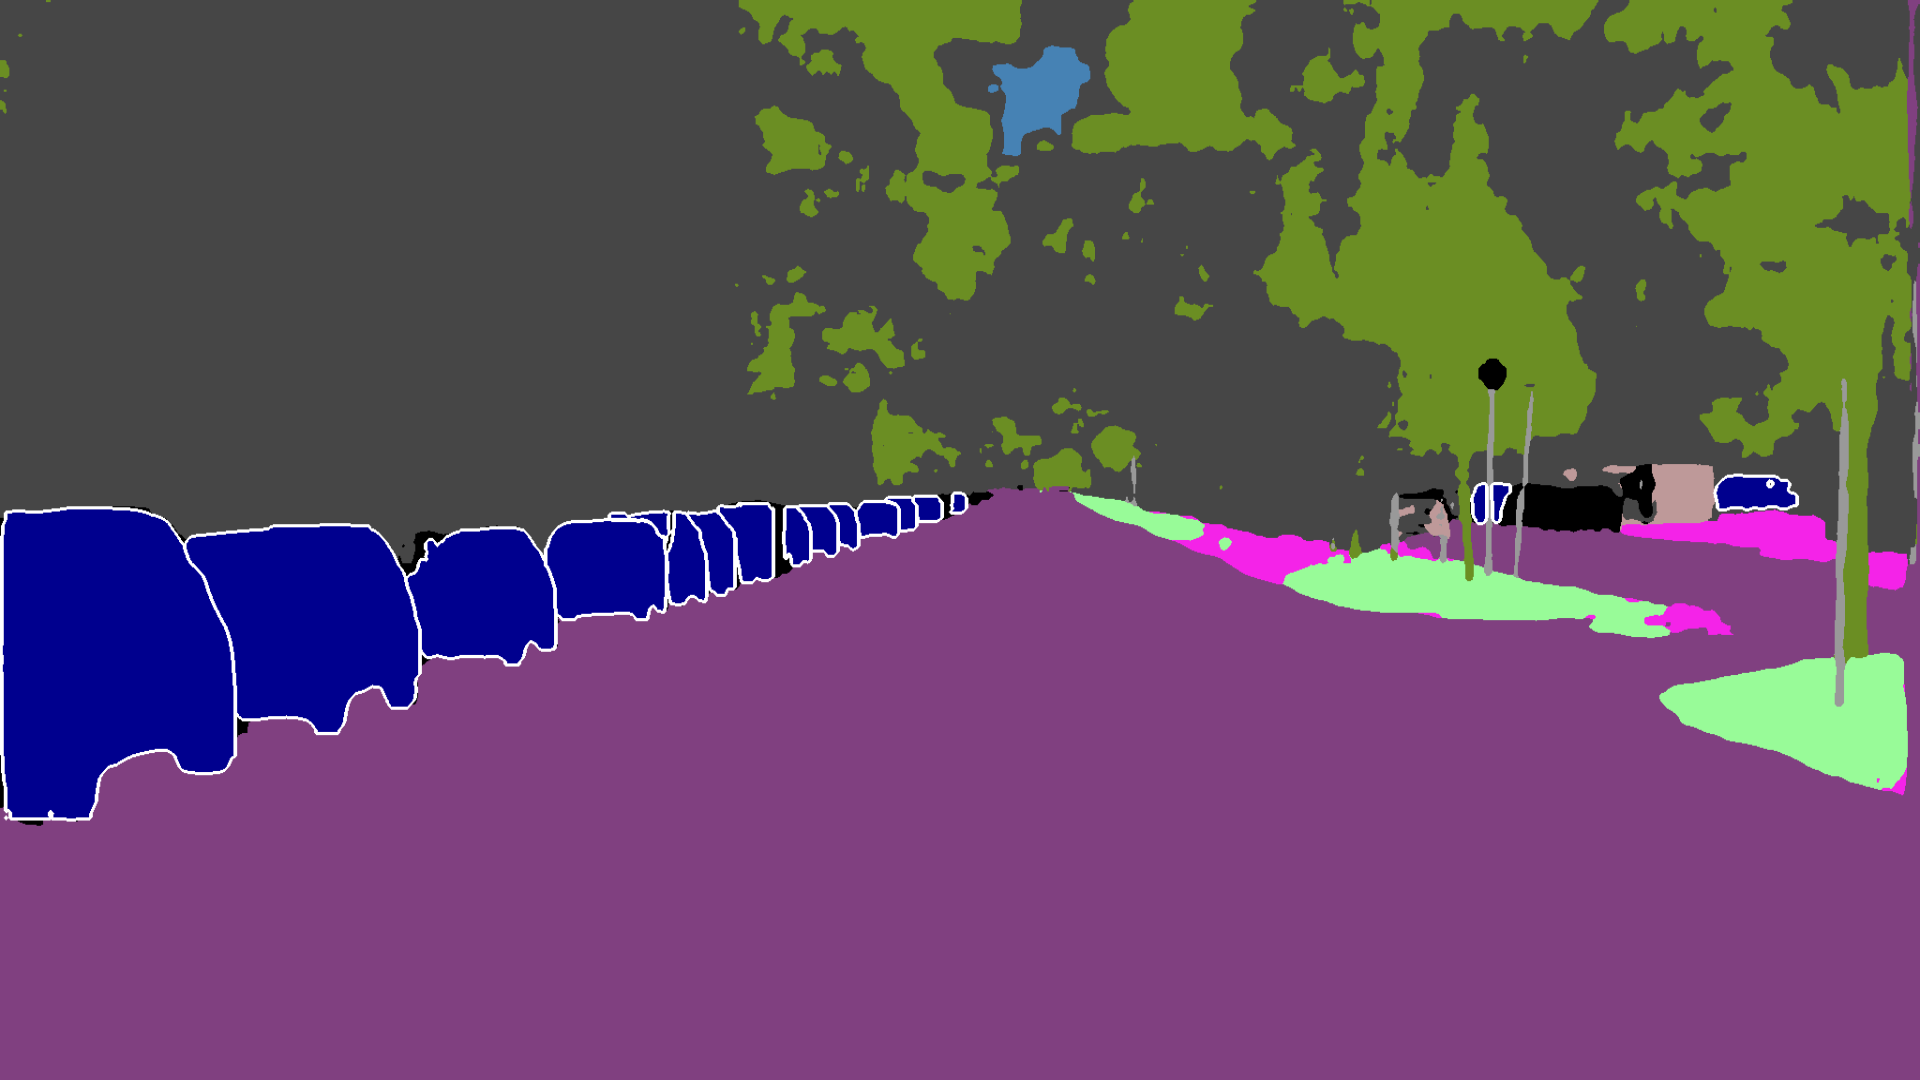
\includegraphics[width=0.6\textwidth]{figures/resultado_primario.png}
    \legend{Fonte: Criação própria}
	\label{fig:resultado_inicial}
\end{figure}

Seguiu-se os passos citados numa publicação no repositório \footnote{\url{https://github.com/DeepSceneSeg/EfficientPS/issues/23}} porém o resultado obtido não foi satisfatório pois não possível discernir quais segmentos pertenciam as respectivas classes, o resultado é ilustrado na \cref{fig:resultado_obtido}.

\begin{figure}[!ht]
	\centering
    \caption{Resultado obtido seguindo os passos da publicação no repositório.}
	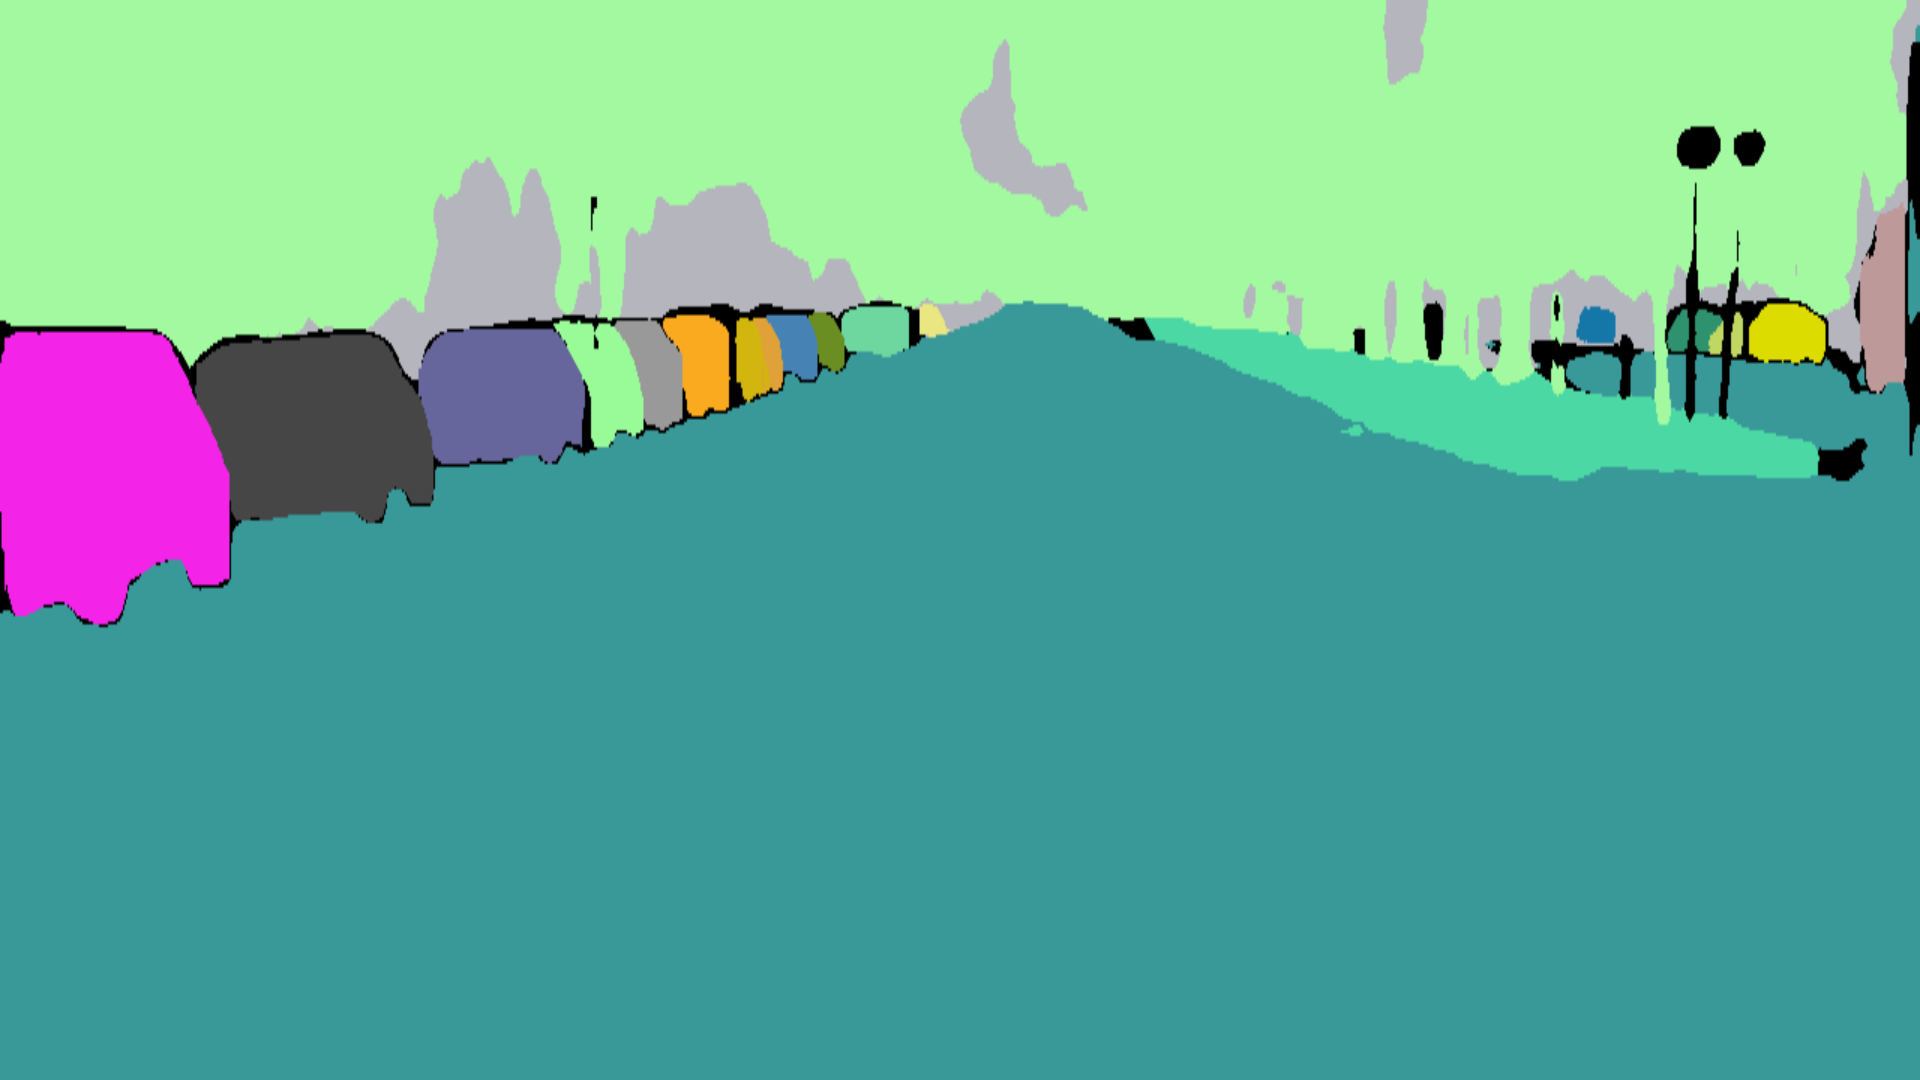
\includegraphics[width=0.6\textwidth]{figures/resultado_obtido.png}
    \legend{Fonte: Criação própria}
	\label{fig:resultado_obtido}
\end{figure}

\subsection{Selecionar contorno}

Para representar a seleção do contorno utilizou-se uma técnica chamada de imagem binária.
A imagem  binária contém  apenas duas cores, geralmente preto e  branco. Pode-se ser utilizada como uma máscara para auxiliar o processamento do  mapa no contorno desejado \cite{Aznag2020}.

Utilizou-se duas maneiras para selecionar o contorno, sendo eles: selecionar por cor e selecionar por preenchimento de inundação — ou  em inglês  flood fill —.

\subsubsubsection*{Selecionar por cor}

O metódo de selecionar por cor se baseia em pegar a cor específica do clique na imagem e percorrer a imagem comparando a cor alvo com a cor da imagem, caso seja a mesma pinte o mesmo pixel da nova imagem como branco e caso não seja pinte como preto.

Uma maneira mais performática de selecionar por cor é definir um espectro de cores e aplicar uma mascára usando o método \textit{inRange} da biblioteca OpenCV, pode-se escolher apenas uma cor.

\subsubsubsection*{Selecionar por preenchimento de inundação}

O método de  selecionar por preenchimento por inundação é um algoritmo de expansão a partir de um pixel, validando se contém a mesma cor.

A implementação inicia uma matriz de zeros com tamanho 2 pixeis maior do que a imagem original.

O clique na  imagem será a semente — ou em inglês  seed — e a partir disso o algoritmo começa uma expansão para os pixeis vizinhos — de cima, baixo, esquerda e direita — caso contenha o mesmo valor de cor pinta de cor branca, e refaz com os pixels marcados  anteriormente até não ter mais o pontos brancos para marcar.

\subsubsubsection*{Tratamento da imagem binária}

Após a saída dos algoritmos de seleção, o objeto selecionado é detectado e centralizado em uma nova imagem, depois recortamos e redimensionamos a partir do centro de forma que fique quadrada. Todos os passos são observáveis na \cref{fig:saidas_selecao}.

\begin{figure}[!ht]
	\centering
    \caption{Passos da seleção da saída da inteligência  artificial.}
	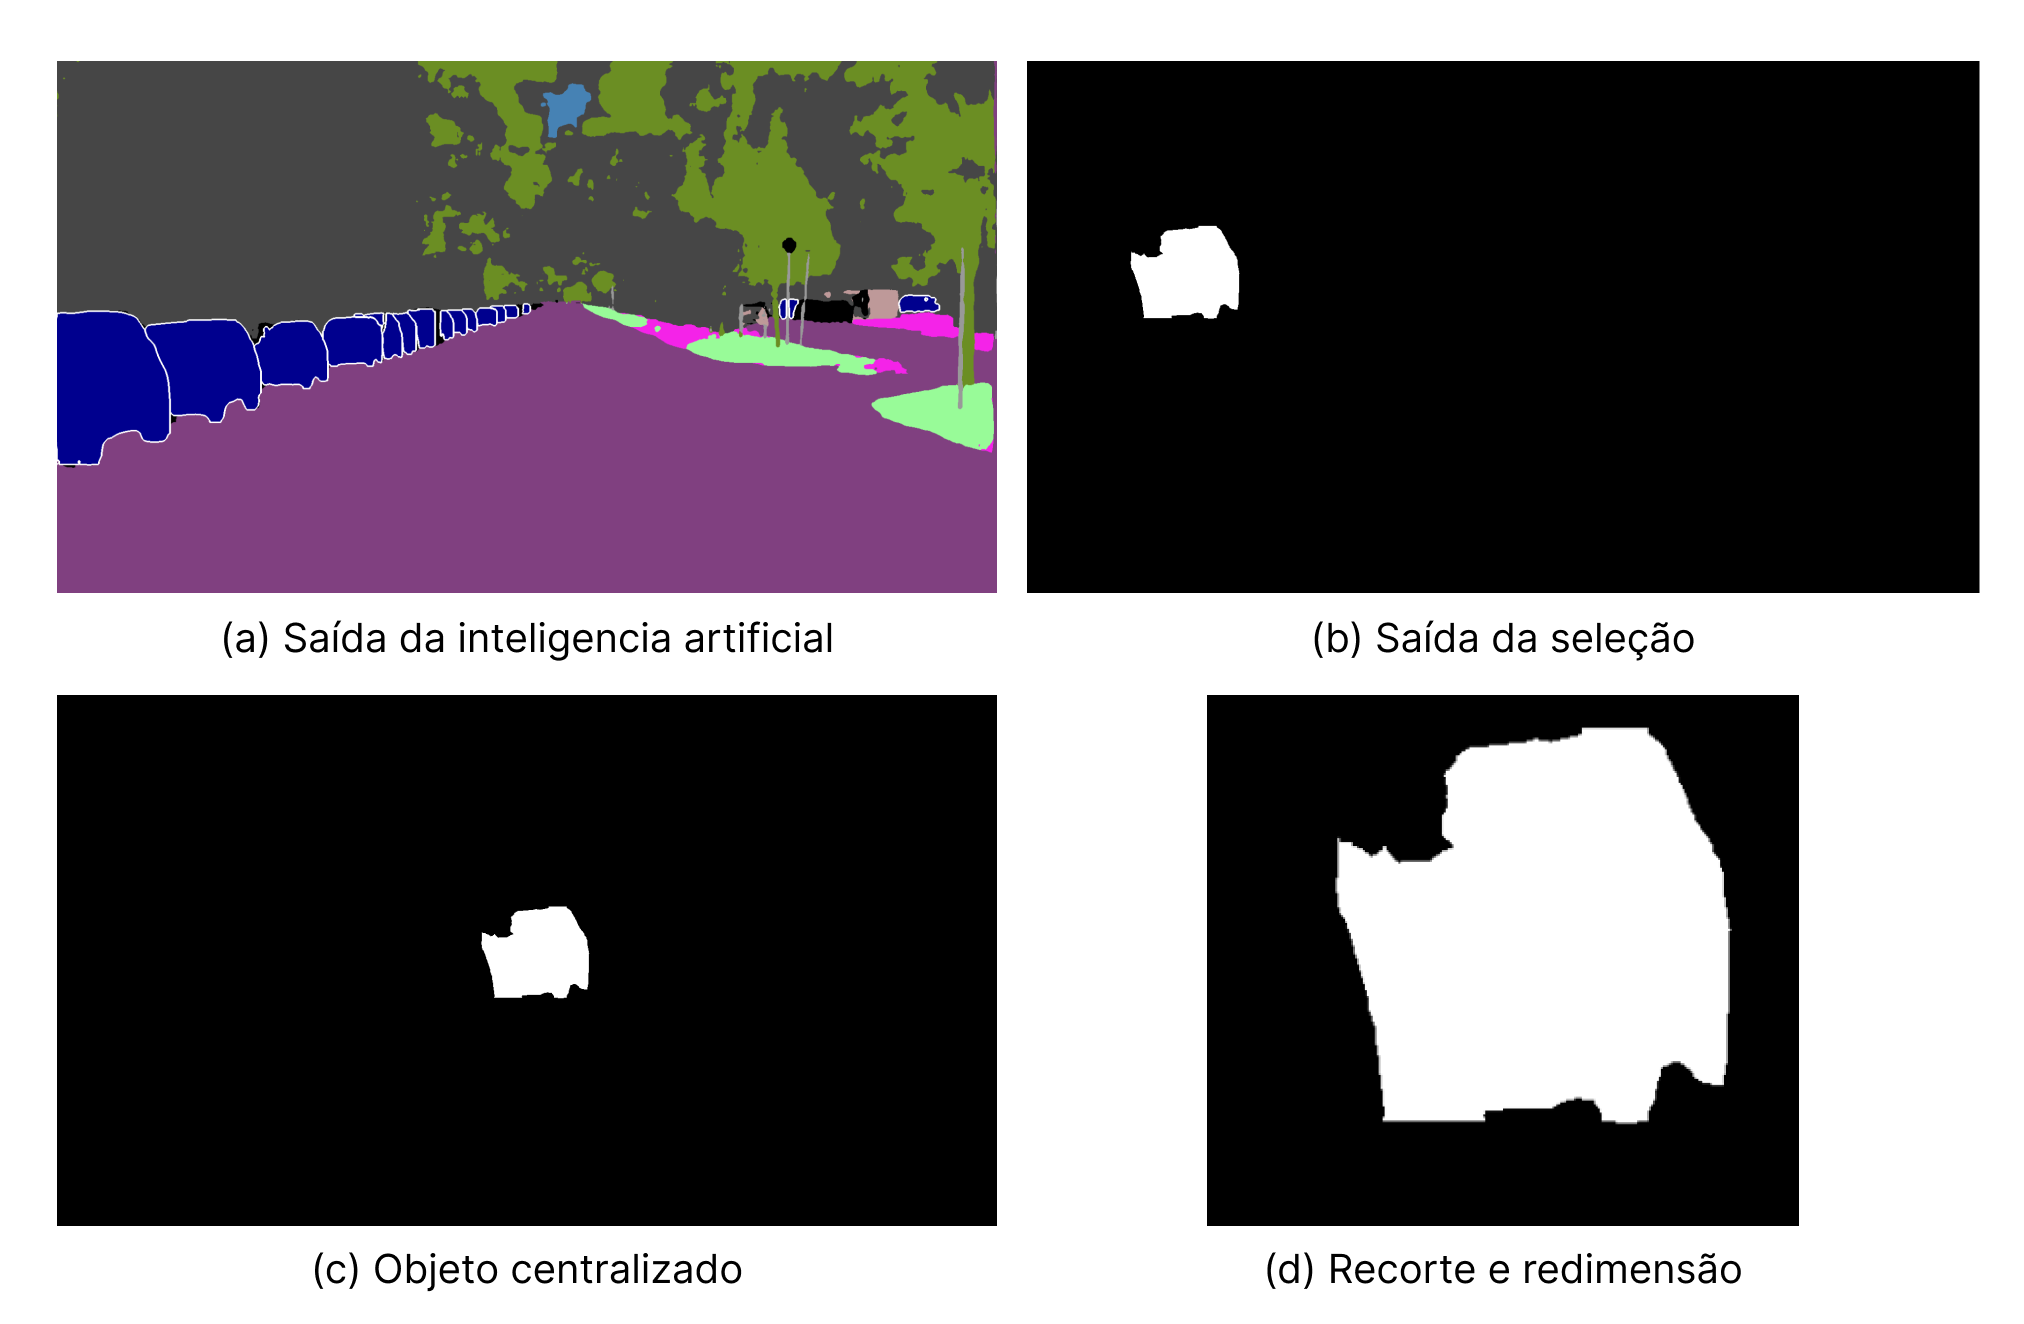
\includegraphics[width=1.0\textwidth]{figures/saidas_selecao.png}
    \legend{Fonte: \space Autoria própria}
	\label{fig:saidas_selecao}
\end{figure}

Porém há uma maneira mais performática para fazer isso, inclusive melhorando os resultados devido ao redimensionamento e a borda não chegarem a um bom cenário. Essa outra maneira usa um método para localizar o objeto na imagem binária e corta a imagem com as cordenadas e dimenões oferecidas. Ápos isso é acrescentado uma borda na altura ou largura com a folga entre as duas, tornando assim a imagem quadricular, depois é redimensionado para manter um padrão e acrescentado mais uma vez uma borda para representar o mar. É possível observar na \cref{fig:saidas_selecao_perf} que o objeto não foi distorcido como na método anterior e manteve-se centralizada na imagem final.

\begin{figure}[!ht]
	\centering
    \caption{Passos da seleção da saída da inteligência  artificial mais performático.}
	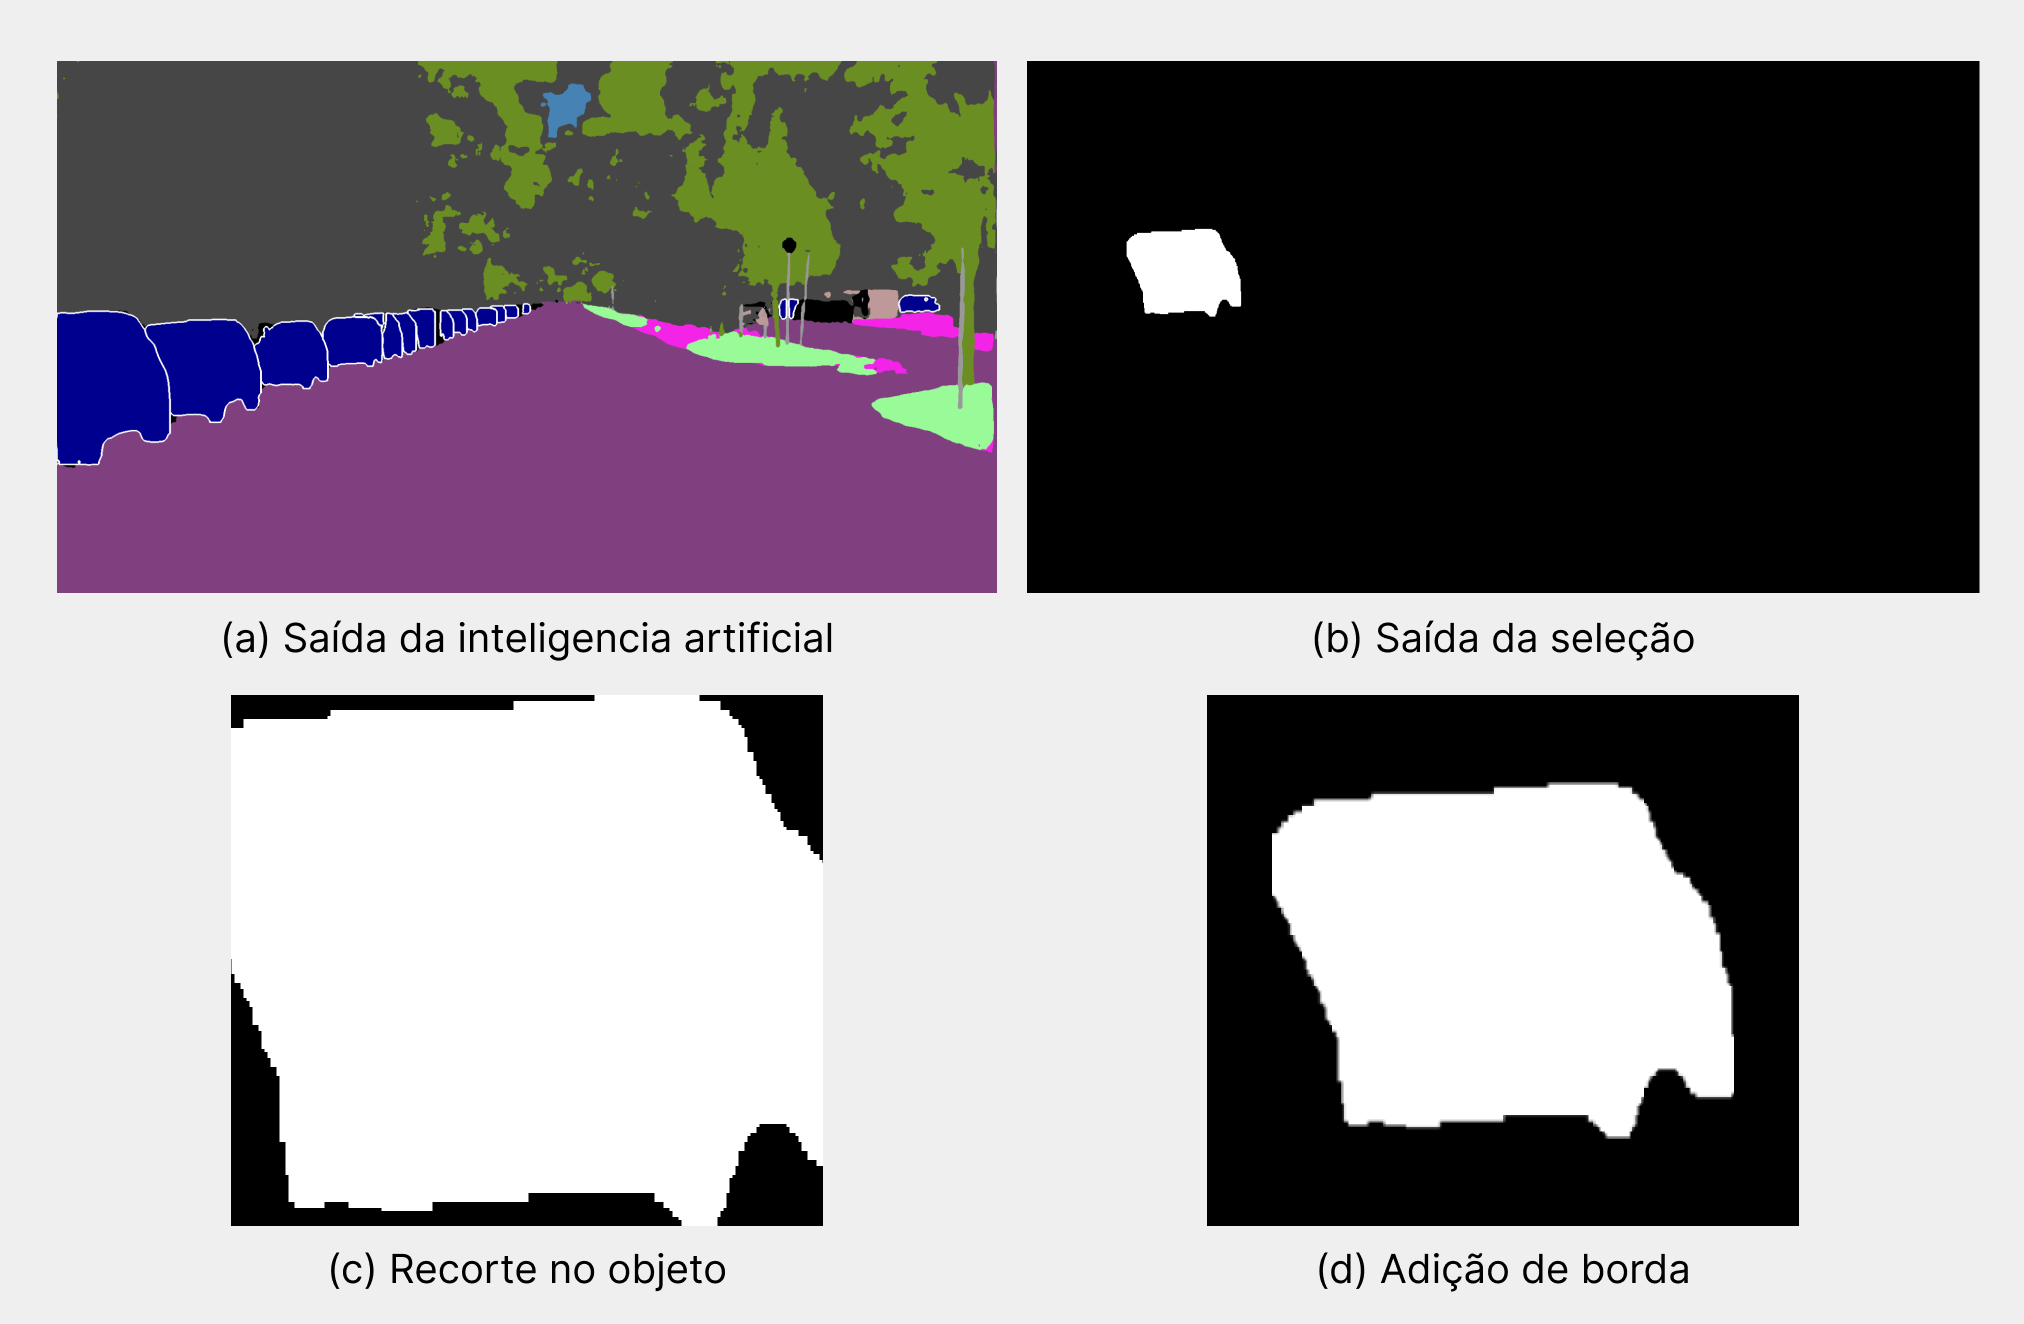
\includegraphics[width=1.0\textwidth]{figures/saidas_selecao_2.png}
    \legend{Fonte: \space Autoria própria}
	\label{fig:saidas_selecao_perf}
\end{figure}

\subsection{Geração procedural do mapa}

Usou-se como base para a geração procedural do mapa o artigo \hyperref[sec:geracaoProcedural]{Polygonal Map Generation for Games} com uma implementação não oficial porém baseada no artigo feito em Python.

\subsubsection{Ilha gerada no contorno}

Para gerar o mapa da ilha é preciso gerar um diagrama de Voronoi. No diagrama primeiro é definido os pontos de quantidade preestabelecida e de localização pseudo-aleatória, esses pontos serão os centroides dos polígonos. Os vértices dos polígonos são gerados a partir da intersecção entre retas perpendiculares aos pontos médios entre os nós vizinhos, logo é criado outro grafo com esses pontos. A definição dos vértices é ilustrada na \cref{fig:explicacao_vértice}, sendo os pontos vermelhos os centroides que são ligados por linhas pretas para gerar pontos médios, representados por pontos amarelos para traçar uma reta perpendicular, depois é calculado a intersecção representado pelo ponto azul que se torna o vértice, e a cor rosa representa a aresta do polígono.

\begin{figure}[!ht]
	\centering
    \caption{Ilustração do cálculo para definir a localização dos vértices.}
	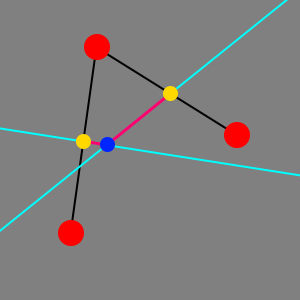
\includegraphics[width=0.6\textwidth]{figures/explicacao_vertice.png}
    \legend{Fonte: \space Autoria própria}
	\label{fig:explicacao_vértice}
\end{figure}

A \cref{fig:diagrama_voronoi_pontos} ilustra o modelo do diagrama de Voronoi do algoritmo, sendo os pontos vermelhos os centroides que são ligados por linhas pretas, os pontos azuis são os vértices que se ligam com linha branca para tornar as arestas formando assim o polígono.

\begin{figure}[!ht]
	\centering
    \caption{Ilustração do diagrama de Voronoi.}
	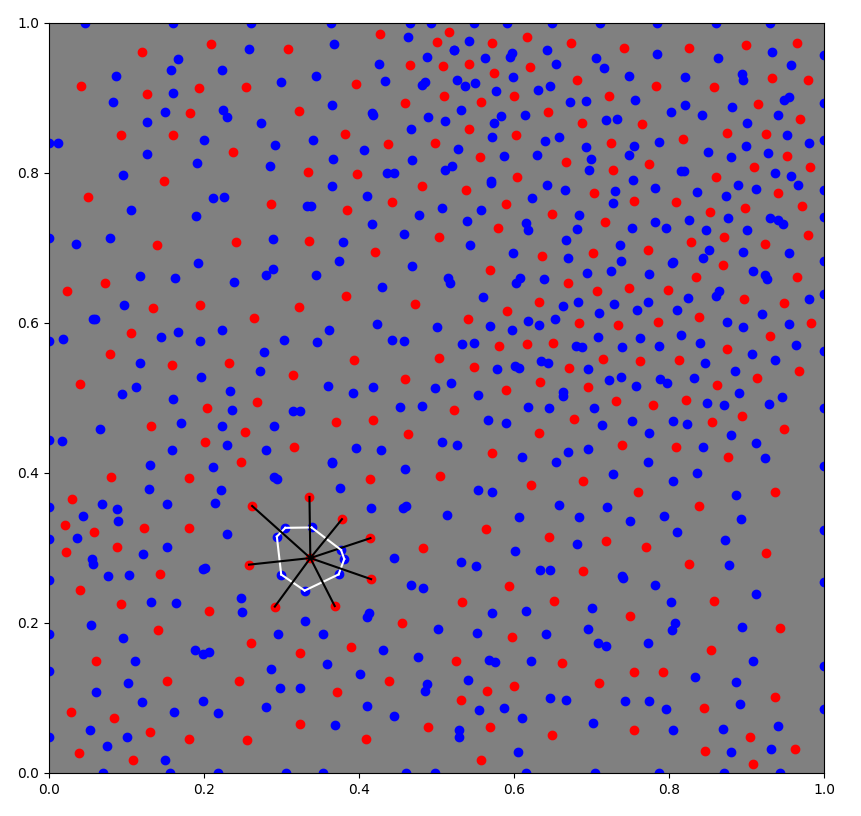
\includegraphics[width=0.6\textwidth]{figures/diagrama_voronoi_pontos.png}
    \legend{Fonte: \space Autoria própria}
	\label{fig:diagrama_voronoi_pontos}
\end{figure}

Cada polígono criado será nomeado de região e basta definir o tipo do terreno, elevação e umidade. Na lógica, marca-se todos os polígonos com o terreno de tipo oceano, depois percorre-se todos os pontos da imagem de entrada e verifica-se se cada pixel que está contido no objeto da imagem binária encontra-se nos polígonos gerados. Se os pontos participarem, marca-se o terreno como tipo terra, e em seguida checa-se em quais polígonos do tipo terra são vizinhos do tipo oceano, se sim, define-se como do tipo litoral, e também assina-se os pontos desses polígonos que encontram-se no polígono do tipo oceano.

Para se calcular a elevação dos polígonos primeiramente é calculado a elevação das arestas de todos os polígonos, isso é feito a partir de uma busca em profundidade que possui o inicio em todas as arestas que tocam a borda do grafico. A toda nova iteração, as arestas que tocam os cantos são atribuidas com o valor 0, e assim defini-se uma evolução da altura conforme chega-se ao centro do mapa.
Após isso é feito o calculo de redistribuição de elevação, que com base na elevação calculada anteriormente é feito uma lista ordenadas pela elevação, começando da menor para a maior. Cada item da lista é enumerado a partir de um índice i e com essa enumeração é calculado usando a \cref{eq:total_indexes}. Após isso é calculado a \cref{eq:vertex_elevation} sendo X a elevação do vértice.
E por final para calcular a elevação do poligino é feito a média dos vértices que pertencem ao polígonos.

\begin{equation}
	\label{eq:total_indexes}
	Y = i / total de indices
\end{equation}

\begin{equation}
	\label{eq:vertex_elevation}
	X = sqrt(fator) - sqrt(sqrt * (1 - Y))
\end{equation}

Para criação dos rios busca-se os vértices do tipo terra e litoral que possuem uma elevação minima definida, ou se os vértices se localizam proximos de um lago, então armazena-se em uma lista. Seleciona-se de forma pseudoaleatória uma quantidade de vértices e verifica-se se o tipo de terreno dos vizinhos dos vértices e das arestas que foram tocados pelos vértices. Para cada um desses é verificado se o tipo de terrenho é terra ou litoral. Após isso, busca-se em todas as arestas a dona do vértice, ao encontrar é marcado como sendo um rio.

Na geração de umidade é atribuído um valor para cada vértice que possui uma aresta do tipo rio, ou se é vizinho de um lago, e é colocado esse item em uma fila. Logo em seguida, busca-se em profundidade, em todos os vértices adjacentes dos itens da fila, e é calculado uma nova umidade a partir de uma multiplicação de um fator com o valor da umidade anteriormente atribuida, e verifica-se se os vértices adjacentes possuem uma umidade maior que a nova umidade calculada, se forem é colocado o vértice adjacente na fila e é atribuido o valor da nova umidade. Para terrenos do tipo oceano é atribuido o valor máximo de umidade.
Por fim, é atribuido o valor da umidade para os polígonos e é redistribuido a umidade a partir de uma lista polígonos com umidades ordenadas, para cada item i executa-se a \cref{eq:umidade} e assim é calculado o valor final da umidade.

\begin{equation}
	\label{eq:umidade}
	i / tamanho(lista) - 1
\end{equation}


Para assinalar os biomas verifica-se o tipo do terreno, altura e a umidade, cada um desses parâmetros liga-se um determinado bioma. E para atribuição final aplica-se a função descrita na \cref{fig:diagrama-whittaker} porém edita-se para chegar nos resultados da \cref{tab:biomes} \space\cite{amitp2010}.

\begin{sidewaystable}
	\centering
	\caption{Relação entre umidade e elevação para biomas}
	\label{tab:biomes}
	\begin{tabularx}{\textwidth}{|X|X|X|X|X|X|X|}
	\hline
	\textbf{Zona de Elevação} & \multicolumn{6}{c|}{\textbf{Zona de Umidade}} \\
	\cline{2-7}
	 & \textbf{6 (úmido)} & \textbf{5} & \textbf{4} & \textbf{3} & \textbf{2} & \textbf{1 (seco)} \\
	\hline
	\textbf{4 (alto)} & \multicolumn{3}{|c|}{NEVE} & TUNDRA & DESNUDO & ESCALDADO  \\
	\hline
	\textbf{3} & \multicolumn{2}{|c|}{TAIGA} & \multicolumn{2}{|c|}{ARBUSTIVO} & \multicolumn{2}{|c|}{DESERTO TEMPERADO} \\
	\hline
	\textbf{2} & FLORESTA TROPICAL TEMPERADA & \multicolumn{2}{|c|}{FLORESTA DECÍDUA TEMPERADA} & \multicolumn{2}{|c|}{GRAMADO} & DESERTO TEMPERADO  \\
	\hline
	\textbf{1 (baixo)} &  \multicolumn{2}{|c|}{FLORESTA CHUVOSA TROPICAL} & \multicolumn{2}{|c|}{FLORESTA SAZONAL TROPICAL} & GRAMADO & DESERTO SUBTROPICAL  \\
	\hline
	\end{tabularx}
\end{sidewaystable}

Para gerar o mapa 3d é gerado uma imagem denominada de mapa de altura, construído com base nos dados de elevações do grafo. Basicamente gera-se uma imagem com tonalidades de cinza sendo o pixel branco com valor 255 o ponto mais alto do mapa e o pixel preto com valor 0 o ponto mais baixo. A \cref{fig:heightmap} ilustra uma saída de mapa de altura.

\begin{figure}[!ht]
	\centering
    \caption{Exemplo de mapa de altura.}
	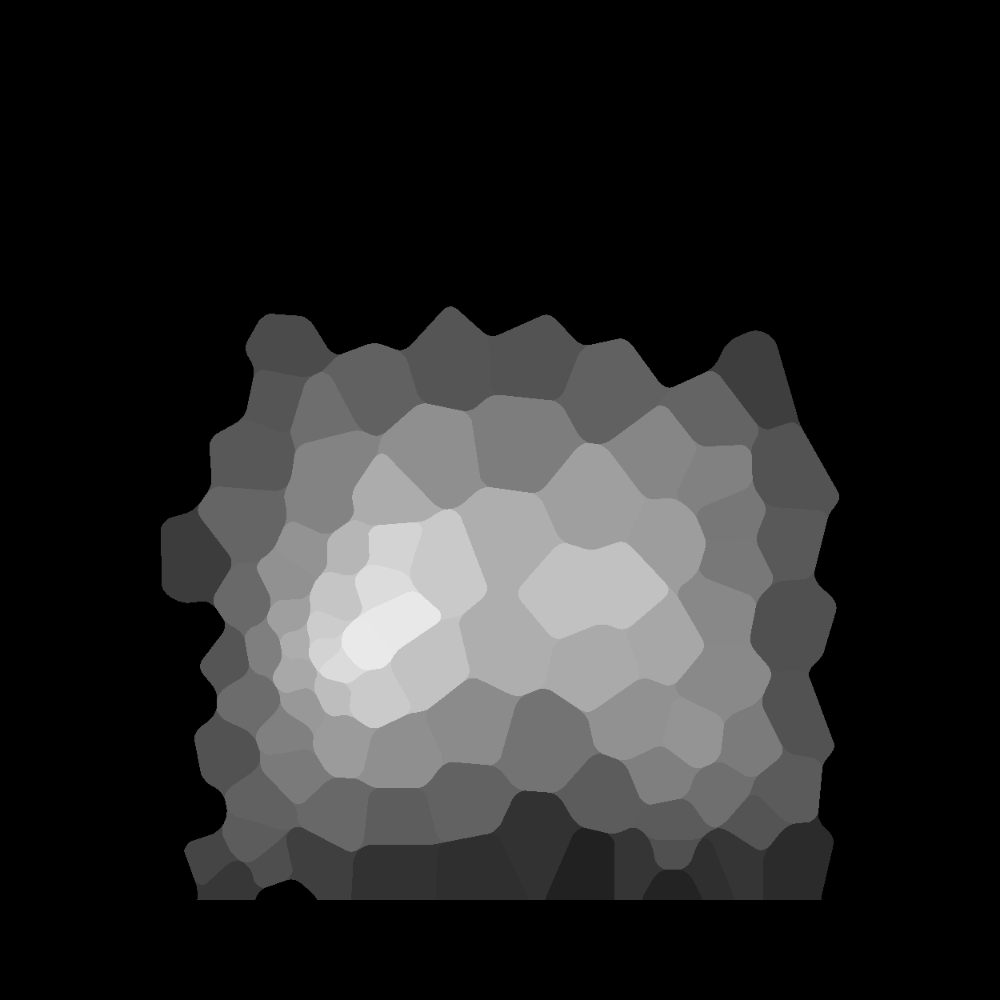
\includegraphics[width=0.6\textwidth]{figures/heightmap_eample.png}
    \legend{Fonte: \space Autoria própria}
	\label{fig:heightmap}
\end{figure}

\subsubsection{Unity - Mapa 3d}

Para demonstrar uma aplicação das imagens utilizou-se o motor gráfico Unity. Criou-se uma automatização entre a geração do mapa e a atualização no projeto Unity. Este processo pode ser dividido em três partes sendo elas o terreno, minimapa em 3d e a jogabilidade.


\subsubsubsection{Terreno}
Para atualizar o terreno usou-se primeiramente o pacote \textit{Terrain Tools} que faciita pois é possível usar um mapa de altura em png ou raw para criar um terreno, ao executar cria-se um terreno no qual o pixel mais branco (255) corresponde a altura mais alta.

Porém esse processo era manual e a ideia era que fosse automatizado, logo utilizou-se um algoritmo ligado a câmera do personagem que toda vez em que inicia-se a cena atualiza-se o terreno com a nova imagem de mapa 3d em raw. O algoritmo abre a imagem e percorre anotando o relevo proporcional a uma matriz e depois aplica no terreno.

Além da funcionalidade de relevo adicionou-se um pacote para alterar a textura de acordo com a altura para diferenciar o oceano da ilha e o bioma de floresta. Utilizou-se o pacote denominado de \textit{Terrain Toolkit 2017}, no script é carregado as texturas e definido alguns parâmetros para atualizar com o terreno.

\subsubsubsection{Minimapa}
A saída da geração procedural visa dois principais resultados, sendo eles: o mapa de altura para definir o terreno e o mapa 2d que pode ser usado como minimapa.

Para usar o mapa 2d como minimapa de forma automatizada foi necessário adicionar nos scripts uma conversão de uma imagem em formato PNG para um Sprite (2D e UI) e atualizar nas propriedades do objeto de jogo. Possibilitando a localização de um ícone representando o jogador nesse minimapa por meio da projeção das coordenadas 3D do mundo do jogo em um mapa 2D.

\subsubsubsection{Jogabilidade}

Criou-se um personagem com movimentação para andar pelo mapa baseado no \footnote{\url{https://www.youtube.com/watch?v=yl2Tv72tV7U}}. Adicionando os objetos e o script principal além de criar uma tag de chão para detectar a colisão é possível jogar no mapa andando em todas as direções e pulando.
\subsection{Testes}

Será feito um teste baseado no sutópico \hyperref[sec:metricas_tecnicas]{métricas e técnicas} no qual irá comparar uma combinação de imagens podendo conter a imagem de entrada do algoritmo de geração procedural ou alguma saída, mapa de altura ou mapa 2d. Em maioria, será utilizado a métrica IoU pois esta é a que pior classifica nosso modelo e também facilita a percepção de melhora, metrificando a semelhança obtida do contorno desejado. Portanto quanto maior essa métrica maior a compatibilidade com o contorno inicialmente proposto.

Dentre essas métricas, será utilizado também uma métrica para o desfoque encontrado em uma imagem, aplica um filtro para detectar bordas em x e y, calcua o gradiente e resulta o desvio padrão. Outra métrica utilizada nos testes foi a duração do tempo no código, medida em segundos e apenas contabilizando a parte de geração procedura dos mapas.

Criou-se um teste genérico para reutiizar em diversos testes e facilitar a reprodução caso algo mude. É definido na chamada do teste quais imagens será feito as métricas, com isso é possível definir todas combinações possíveis. Para cada combinação será executado 5 imagens de entrada pré-definidas e em cada imagem irá percorrer um laço baseado em algum modificador sendo eles, tamanho do filtro de desfoque, quantidade de pontos ou tamanho da borda no mapa 2d, em cada iteração do parâmetro modificador será executado três vezes.

Em cada iteração de todos esses laços aninhados será gerado proceduralmente algum mapa ou os dois, processado as métricas e armazenado, após isso será calculado a média das métricas e criado uma tabela em latex como resultado.

\subsection{Pós processamento}
Analisando-se o resultado gerado no Unity do mapa 3d na \cref{fig:unity_init} percebe-se que não existe uma harmonia entre os biomas e por isso gerou-se uma solução aplicando um desfoque na imagem de mapa de altura para suavizar a mudança de biomas.

\begin{figure}[!ht]
	\centering
    \caption{Resultado no unity sem usar filtro de desfoque no mapa de altura.}
	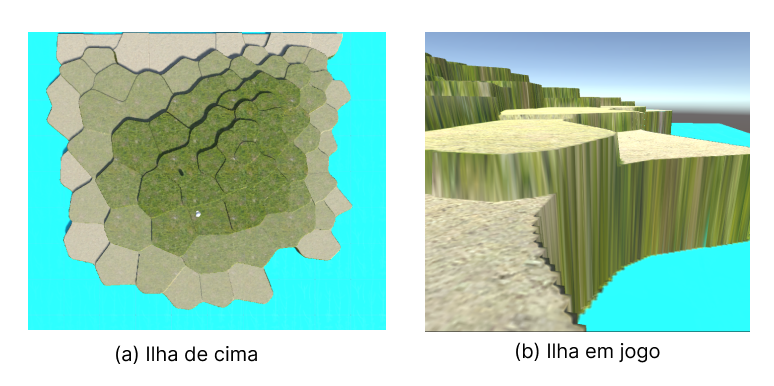
\includegraphics[width=0.8\textwidth]{figures/unity_entry.png}
    \legend{Fonte: \space Autoria própria}
	\label{fig:unity_init}
\end{figure}

Aplicando um filtro — ou kernel — de desfoque com tamanho 100x100, obteve-se o resultado ilustrado na \cref{fig:unity_blur}. Porém se analisar a \cref{tab:blur_error_input_output_3d} pode-se observar que o resultado piorou as métricas, conclui-se que o desfoque piorou a qualidade de equivalência de contornos, aumentando um problema de escala, visto que apenas o erro do mapa de altura foi encontrado. Na \cref{fig:comparando_blur} observa-se uma representação visual dos conjuntos definidos no \hyperref[sec:classificacao_conjuntos]{sub tópico}.

\begin{figure}[!ht]
	\centering
    \caption{Resultado no unity usando filtro de desfoque no mapa de altura.}
	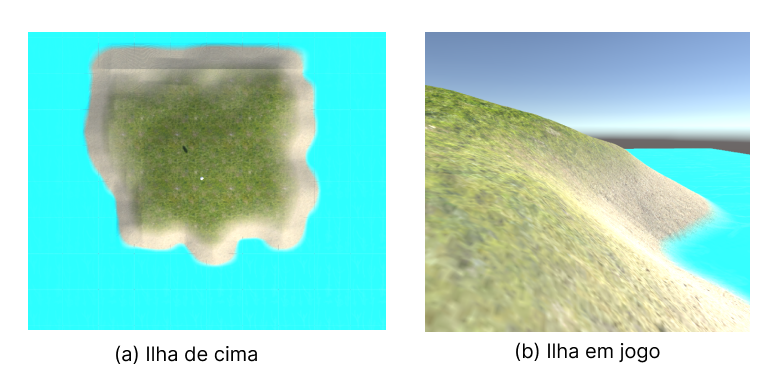
\includegraphics[width=0.8\textwidth]{figures/unity_blur.png}
    \legend{Fonte: \space Autoria própria}
	\label{fig:unity_blur}
\end{figure}

\begin{table}[h]
            \centering
            \caption{Resultados dos testes de contorno}
            \label{tab:resultados-contorno}
            \begin{tabular}{|c|c|c|}
                \hline
                                Tamanho filtro & IoU & Blur \\
                \hline
                0 & 0.7385 & 53.49246\\
        100 & 0.60484 & 9.75581\\
                \hline
            \end{tabular}
        \end{table}




\begin{figure}[!ht]
	\centering
    \caption{Ilustração da classificação de conjuntos entre a iamgem de entrada e o mapa de altura}
	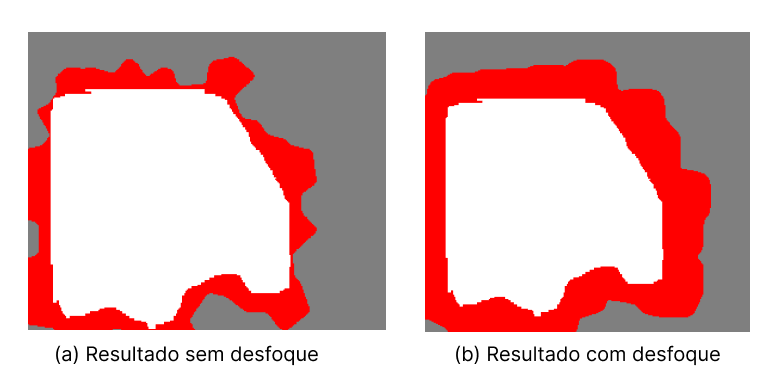
\includegraphics[width=0.8\textwidth]{figures/comparacao_blur.png}
    \legend{Fonte: \space Autoria própria}
	\label{fig:comparando_blur}
\end{figure}

Logo para tratar esse problema adotou-se uma solução baseada em redimensionar a imagem e adicionar uma borda para que diminui-se assim o tamanho do mapa de altura. Portanto foi redimensionado uma imagem 1000x1000 para 800x800, reduzindo em 20\% e depois adicionado uma borda de cor preta em todos os lados de tamanho 100, logo retorna ao tamanho original. E para encontrar o melhor tamanho do filtro de desfoque para essas condições executou-se os testes alterando o tamanho do filtro apos a aplicação da técnica de diminuir o tamanho do mapa. Os resultados referentes aos testes encontram-se na \cref{tab:blur_solution_input_output_3d}. Para selecionar o melhor resultado definiu-se a quesito de ter a menor métrica de desfoque — que significa ter mais desfoque na imagem — e com a métrica IoU que varie no máximo 1\% da métrica sem o filtro de desfoque. Logo seleciona-se o restultado de filtro de tamanho 80 pois a métrica IoU tem 79\% assim como o tamanho de filtro 0. Percebe-se também que com a diminuição da borda resultou no comparrtilhamento entre os erros da imagem de entrada com o mapa de altura.

\begin{table}[h]
    \centering
    \caption{Resultados dos testes entre imagem de entrada e output3d}
    \label{tab:blur_solution_input_output_3d}
    \begin{tabular}{|c|c|c|c|c|}
        \hline
        Tamanho filtro & Desfoque & IoU & FDR & FNR \\
        \hline
        100 & 11.35778 & 0.76178 & 0.22752 & 0.01707\\
        90 & 11.88265 & 0.76887 & 0.2162 & 0.02281\\
        80 & 12.37601 & 0.79299 & 0.18761 & 0.02824\\
        70 & 13.59314 & 0.79101 & 0.18298 & 0.03676\\
        60 & 14.75522 & 0.80283 & 0.16196 & 0.04787\\
        50 & 16.29726 & 0.81851 & 0.13458 & 0.06073\\
        40 & 18.35148 & 0.81608 & 0.12325 & 0.07635\\
        30 & 21.52558 & 0.81866 & 0.10467 & 0.0935\\
        20 & 27.79682 & 0.8183 & 0.08627 & 0.11246\\
        10 & 38.13084 & 0.80744 & 0.07181 & 0.13757\\
        0 & 48.89338 & 0.79895 & 0.05978 & 0.15749\\
        \hline
    \end{tabular}
\end{table}




Após melhorar o resultado do mapa de entrada é necessário ajustar o mapa 2d visto que esse deve ser bem parecido com o mapa de altura, parar informar por exemplo a localização exata do personagem em jogo com visualização do mapa inteiro. Observa-se na \cref{tab:border_2d_solution_output_2d_output_3d} os resultados obtidos dos testes com o tamanho da borda adicionada ao mapa 2d e o maior valor de IoU obtido foi 60.

\begin{table}[h]
    \centering
    \caption{Resultados dos testes entre mapa 2d e mapa de altura}
    \label{tab:border_2d_solution_output_2d_output_3d}
    \begin{tabular}{|c|c|c|c|}
        \hline
        Tamanho borda & IoU & FDR & FNR \\
        \hline
        0 & 0.82075 & 0.02435 & 0.16192\\
        10 & 0.84148 & 0.02679 & 0.13833\\
        20 & 0.86438 & 0.03616 & 0.10622\\
        30 & 0.87938 & 0.04263 & 0.0846\\
        40 & 0.89456 & 0.05307 & 0.0578\\
        50 & 0.90031 & 0.06612 & 0.03827\\
        60 & 0.90771 & 0.07929 & 0.0152\\
        70 & 0.89229 & 0.10441 & 0.00408\\
        80 & 0.86867 & 0.13132 & 1e-05\\
        90 & 0.84037 & 0.15963 & 0.0\\
        100 & 0.81396 & 0.18604 & 0.0\\
        \hline
    \end{tabular}
\end{table}




\subsection{Interface gráfica}

Utilizou-se a biblioteca PyQt5 para criar uma interface gráfica na qual o usuário poderá interagir e criar um mapa a partir da seleção do contorno detectado pelo modelo de IA.

Esse módulo é responsável para conectar todas as partes e obter o mapa. Portanto é necessário abrir uma imagem do diretório local, carregar e disparar a execução do processo de segmentação de imagem. Após o resultado da IA, permitir a seleção do contorno,  criar uma imagem binária a partir do contorno e envia-lá como argumento na geração procedural de mapas.

Além disso para promever a usabilidade utilizou-se um loading específico para PyQt5 e para isso teve-se que usar threads, criando classes para rodar as tarefas de forma separada e síncrona.

\chapter{Resultados}

Neste capítulo é apresentado os resultados obtidos da implementação e discutido o  impacto e possíveis causas.

\section{Apresentação}

Para apresentar os resultados será abordado tabelas contendo testes com todas combinações de imagens, uma imagem com os resultados finais das tabelas além de uma imagem com todos os passos da aplicação

A Tabela \ref{tab:final_input_output_2d} apresenta os resultados comparativos entre a imagem de entrada e o mapa 2D. Esta comparação é realizada utilizando a técnica de classificação de conjuntos conforme definido por \cite{kirillov2019panoptic}. A análise foca na avaliação das métricas conforme o número de pontos no diagrama de Voronoi, incluindo União sobre Interseção (IoU), Acurácia (Acc), F1 Score (F1), Coeficiente de Correlação de Matthews (MCC), Taxa de Descoberta Falsa (FDR), Taxa de Falso Negativo (FNR) e o tempo de execução do código \cite{Chicco2020, confusion_matrix_calculator, iou_metric_link}.

Esta tabela é crucial, pois ela evidencia, com base em dados concretos, a semelhança do mapa 2D com o contorno do mapa de entrada. Além disso, corrobora a hipótese de que um maior número de pontos no mapa leva a melhores resultados nas métricas de IoU, Acc, F1 e MCC (onde valores mais altos indicam melhor desempenho), e simultaneamente, a uma redução nos índices de FDR e FNR (onde valores menores são preferíveis, visto que representam menor erro). Observa-se, ainda, que um aumento no número de pontos implica em um maior tempo de processamento na geração procedural do mapa.


\begin{table}[h]
	\centering
	\caption{Resultados dos testes entre imagem de entrada e mapa 2d}
	\label{tab:final_input_output_2d}
	\begin{tabular}{|c|c|c|c|c|c|c|c|}
		\hline
						Pontos & IoU & Acc & F1 & MCC & FDR & FNR & Duração \\
		\hline
		50 & 0.71361 & 0.86085 & 0.8323 & 0.74079 & 0.2762 & 0.01923 & 5.33293\\
100 & 0.80033 & 0.9151 & 0.88857 & 0.82809 & 0.17938 & 0.0292 & 10.0857\\
150 & 0.83825 & 0.93506 & 0.91168 & 0.86398 & 0.13792 & 0.03125 & 15.32477\\
200 & 0.85695 & 0.94434 & 0.92268 & 0.88059 & 0.10822 & 0.04269 & 20.22667\\
250 & 0.868 & 0.94946 & 0.92908 & 0.89029 & 0.09454 & 0.04525 & 27.26459\\
300 & 0.87405 & 0.95241 & 0.93263 & 0.89612 & 0.08326 & 0.04984 & 33.46705\\
		\hline
	\end{tabular}
\end{table}


Os resultados obtidos na \cref{tab:final_input_output_3d} derivam da comparação entre a imagem de entrada e o mapa de altura, utilizando a técnica de classificação de conjuntos conforme definida por \cite{kirillov2019panoptic}. Essa comparação foi realizada para mensurar diversos aspectos, incluindo as métricas associadas ao número de pontos no diagrama de Voronoi. As métricas abrangem União sobre Interseção (IoU), Acurácia (Acc), F1 Score (F1), Coeficiente de Correlação de Matthews (MCC), Taxa de Descoberta Falsa (FDR), Taxa de Falso Negativo (FNR) e a duração da execução do código \cite{Chicco2020, confusion_matrix_calculator, iou_metric_link}.

A relevância dessa tabela reside na capacidade de demonstrar, por meio de dados concretos, a proximidade entre o mapa de altura e o contorno do mapa de entrada. Além disso, ela valida a hipótese de que o aumento no número de pontos resulta em melhores desempenhos nas métricas IoU, Acc, F1 e MCC, indicando uma maior semelhança entre os mapas. Simultaneamente, observa-se uma diminuição nas métricas FDR e FNR, evidenciando uma redução nos erros. Vale notar que a quantidade de pontos também impacta diretamente na duração da geração procedural do mapa, sendo um fator relevante a ser considerado.

\begin{table}[h]
	\centering
	\caption{Resultados dos testes entre imagem de entrada e mapa de altura}
	\label{tab:final_input_output_3d}
	\begin{tabular}{|c|c|c|c|c|c|c|c|}
		\hline
						Pontos & IoU & Acc & F1 & MCC & FDR & FNR & Duração \\
		\hline
		50 & 0.67955 & 0.83753 & 0.80827 & 0.70471 & 0.31036 & 0.02058 & 5.29547\\
100 & 0.74929 & 0.88637 & 0.85581 & 0.77953 & 0.23518 & 0.02501 & 9.822\\
150 & 0.79092 & 0.91133 & 0.88236 & 0.82054 & 0.18669 & 0.0319 & 15.43131\\
200 & 0.80368 & 0.91818 & 0.89056 & 0.83234 & 0.17252 & 0.03302 & 21.06372\\
250 & 0.82316 & 0.92831 & 0.90248 & 0.85016 & 0.14821 & 0.03784 & 25.92615\\
300 & 0.82598 & 0.93022 & 0.90415 & 0.85286 & 0.14182 & 0.04223 & 32.75651\\
		\hline
	\end{tabular}
\end{table}

A tabela referenciada como \cref{tab:final_output_2d_output_3d} apresenta os resultados comparativos entre o mapa de altura e sua representação em mapa 2D. Esta comparação é realizada através do método de classificação de conjuntos proposto por \cite{kirillov2019panoptic}, avaliando os resultados com base em várias métricas conforme a quantidade de pontos no diagrama de Voronoi. As métricas avaliadas incluem União sobre Interseção (IoU), Acurácia (Acc), F1 Score (F1), Coeficiente de Correlação de Matthews (MCC), Taxa de Descoberta Falsa (FDR), Taxa de Falso Negativo (FNR) e o tempo de execução do código \cite{Chicco2020, confusion_matrix_calculator, iou_metric_link}. Esta tabela é crucial para demonstrar que o mapa de altura (que irá se tornar o mapa 3d) com o mapa 2D se assemelham, pois no protótipo do Unity servirá para localização do personagem, combinando o mapa 2d como minimapa e o mapa 3d com dimensão e profundidade. Observa-se também que um aumento no número de pontos resulta em maior tempo de geração procedural do mapa.

\begin{table}[h]
	\centering
	\caption{Resultados dos testes entre mapa 2d e mapa de altura}
	\label{tab:final_output_2d_output_3d}
	\begin{tabular}{|c|c|c|c|c|c|c|c|}
		\hline
						Pontos & IoU & Acc & F1 & MCC & FDR & FNR & Duração \\
		\hline
		50 & 0.91515 & 0.9589 & 0.95559 & 0.91721 & 0.06528 & 0.0222 & 5.0949\\
100 & 0.90352 & 0.95708 & 0.94924 & 0.91312 & 0.08082 & 0.01838 & 10.08713\\
150 & 0.90342 & 0.9592 & 0.94915 & 0.91636 & 0.08265 & 0.01631 & 14.82656\\
200 & 0.90421 & 0.96087 & 0.94955 & 0.91901 & 0.08312 & 0.01487 & 20.51247\\
250 & 0.90505 & 0.96207 & 0.95004 & 0.92088 & 0.08284 & 0.0142 & 26.63407\\
300 & 0.90357 & 0.96252 & 0.94921 & 0.92112 & 0.08565 & 0.01276 & 33.59293\\
		\hline
	\end{tabular}
\end{table}

A \cref{fig:result_final} contém a ilustração da classificação dos conjuntos de cada combinação, logo a imagem a, tem a ilustração da última execução da combinação entre imagem de entrada e o mapa 2d dos resultados da \cref{tab:final_input_output_2d}, a imagem b, tem a ilustração da última execução da combinação entre imagem de entrada e o mapa de altura dos resultados da \cref{tab:final_input_output_3d}, já a imagem c, tem a ilustração da última execução da combinação entre imagem de altura e o mapa 2d dos resultados da \cref{tab:final_output_2d_output_3d}.

\begin{figure}[!ht]
	\centering
    \caption{Resultados da última execução de cada combinação de imagens.}
	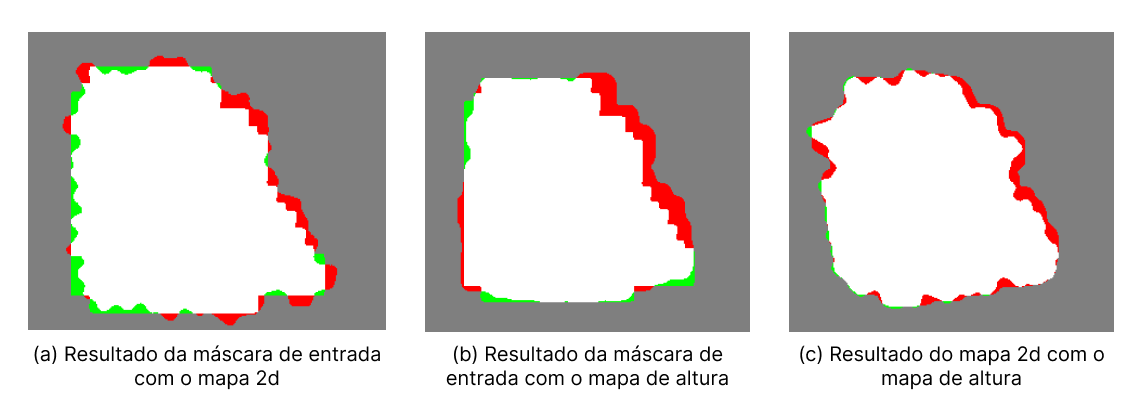
\includegraphics[width=\textwidth]{figures/comb_results_final.png}
    \legend{Fonte: \space Autoria própria}
	\label{fig:result_final}
\end{figure}

A \cref{fig:combs_result} contém todos os passos da execução do programa gerado em Python. Sendo a imagem a, uma captura de tela da interface gráfica com PyQt5, a imagem b, é uma captura de tela abrindo uma imagem para ser segmentada, na imagem c, é uma captura de tela rodando o EfficientPS na imagem que foi escolhida, na imagem d, tem uma captura de tela da saída da segmentação panóptica pelo modelo EfficientPS, na imagem e, tem o carregamento pós seleção do usuário que no caso selecionou um carro com o método de preenchimento por inundação, na imagem f, tem o resultado do mapa 2d com o contorno selecionado anteriormente, na imagem g, tem uma captura de tela da automação usando Unity para atualizar um terreno com o mapa de altura de saída da geração procedural, e por fim a imagem h, tem uma captura de tela do Unity rodando a aplicação e abrindo o minimapa (usando o mapa 2d) para ter uma noção de localização no mapa em 3d usando um ponto para marcar a localização atual do personagem no minimapa (mapa 2d).

\begin{figure}[!ht]
	\centering
    \caption{Passos do programa final.}
	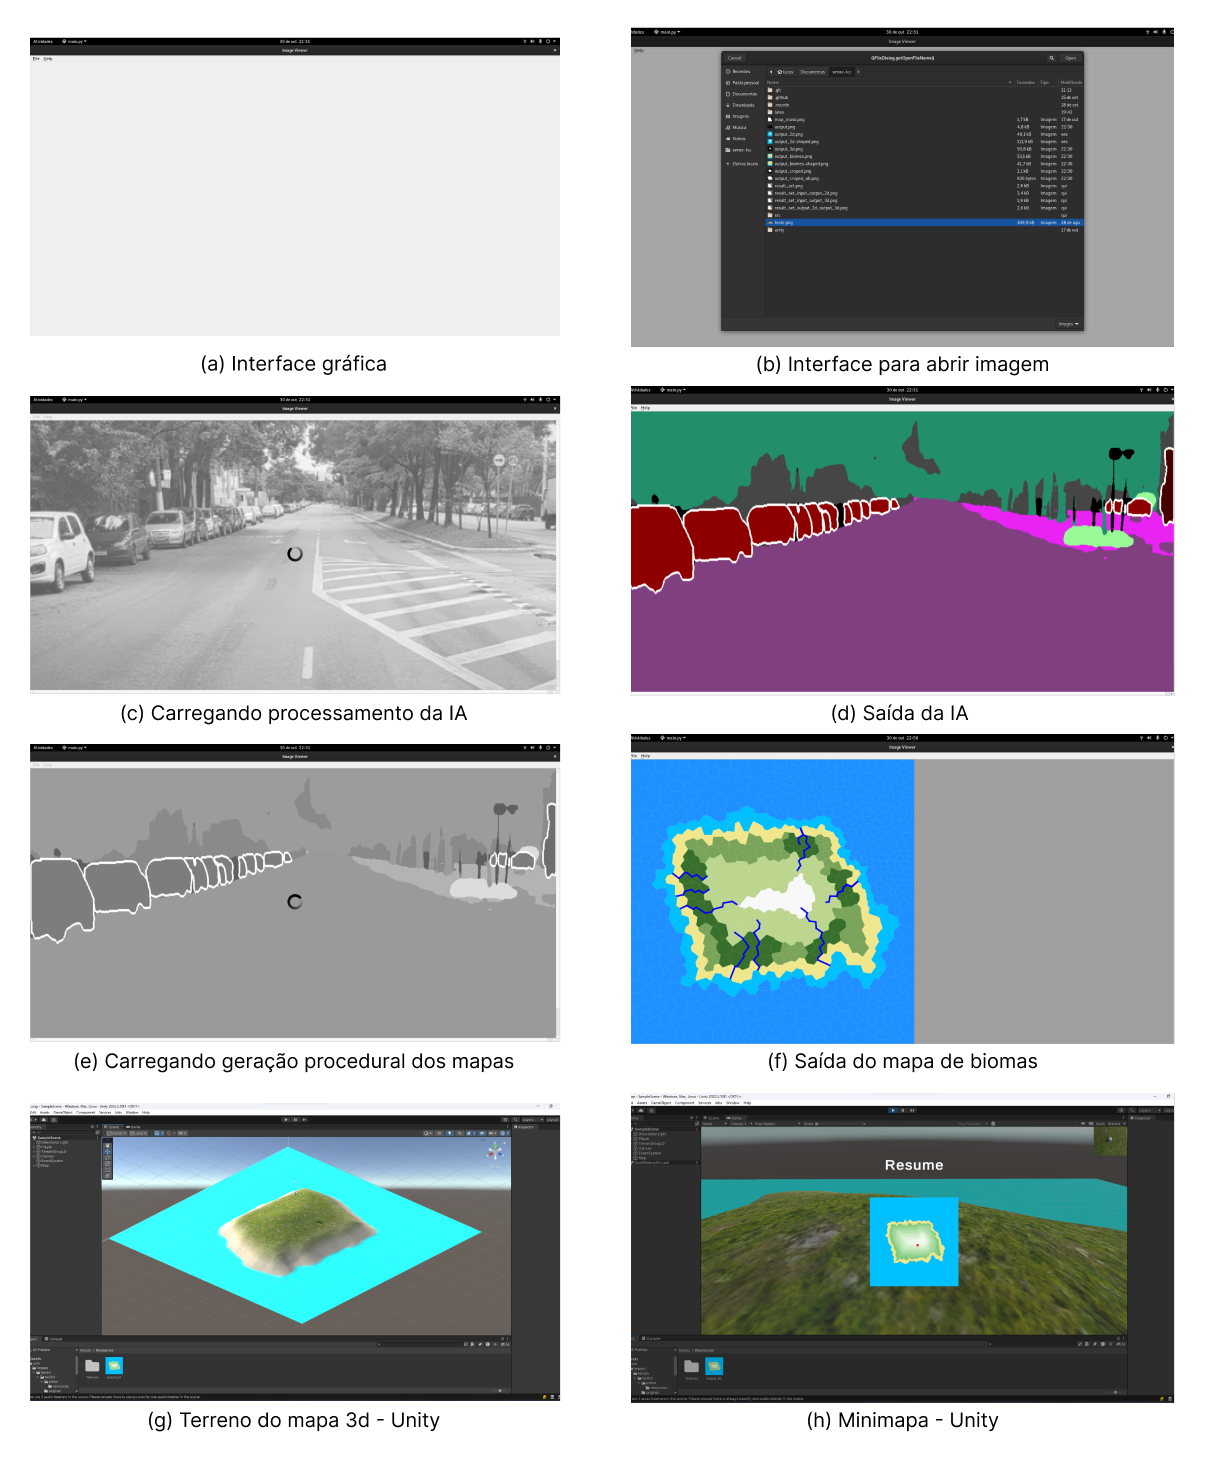
\includegraphics[width=\textwidth]{figures/result_final.png}
    \legend{Fonte: \space Autoria própria}
	\label{fig:combs_result}
\end{figure}

\section{Analise dos resultados}

\chapter{Considerações finais}

Neste capítulo é desenvolvido as conclusões do trabalho e trabalhos futuros para evoluir com a ciência na tentativa de conseguir resultados melhores.

\section{Conclusão}

\section{Trabalhos futuros}

As seguintes propostas podem ser estudadas e aplicadas para aprimorar os resultados obtidos:

\begin{itemize}
    \item Utilizar um modelo de segmentação panóptica com suporte multiplataforma
    \item Utilizar paralelismo para melhorar  o tempo de execução
    \item Utilizar rasterização para melhorar  o tempo de execução
    \item Testar tempo de execução com outros métodos de geração procedural visando um mapa baseado em um contorno
\end{itemize}

% \section{Cronograma}

O processo de desenvolvimento será separado em 3 tópicos principais, inteligência artificial, diagrama de Voronoi e interface de usuário. O desenvolvimento de cada tópico do software será feito em paralelo, pois os tópicos não possuem acoplamento.

\subsection*{inteligência Artificial}

Será necessário decidir quais conjuntos de dados utilizar, o modelo está pronto e disponível no GitHb \cite{mohan2020efficientps} portanto será necessário treinar o modelo e avalia-lo com base na métrica PQ \cref{eq:pq_metric}.

As especificações do modelo proposto são: Linux, Python 3.7, PyTorch 1.7, CUDA 10.2, GCC 7 ou 8 além dos pacotes inseridos no arquivo requirements.txt.

O tempo estimado para o desenvolvimento é de 1 a 2 meses, a maior parte será para treinar e validar o resultado.

\subsection*{Diagrama de Voronoi}

Para o desenvolver código do diagrama de Voronoi será preciso primeiro gerar os pontos e desses pontos as áreas, fazer o algoritmo entender se a área tocou no segmento de imagem, caso tenha tocado armazenar para um processamento posterior que irá especificar qual bioma aquela áreas será, para fazer os teste será necessário uma imagem com um polígono.

O tempo estimado para o desenvolvimento é de 1 mes.

\subsection*{Interface de Usuário}

A interface de usuário terá 5 telas principais, inicio, processamento da segmentação, seleção, processamento de seleção, resultado. 

As telas terão o seguinte fluxo:

\begin{figure}[H]
	\centering
    \caption{Tela de início, botões de carregar imagem e carregar projeto, menu de contexto arquivos com 3 botões, carregar imagem, carregar projeto e salvar.}
	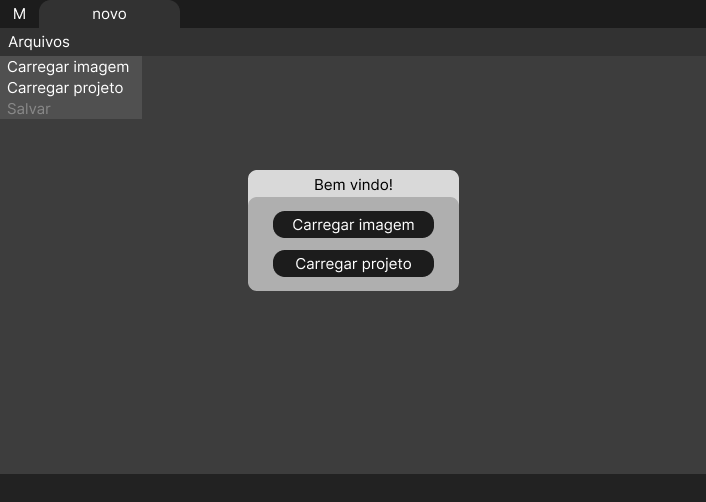
\includegraphics[width=0.6\textwidth]{figures/tela_novo.png}
    \legend{Fonte: Criação própria}
	\label{fig:tela_novo}
\end{figure}


\begin{figure}[H]
	\centering
    \caption{Tela de processamento da segmentação}
	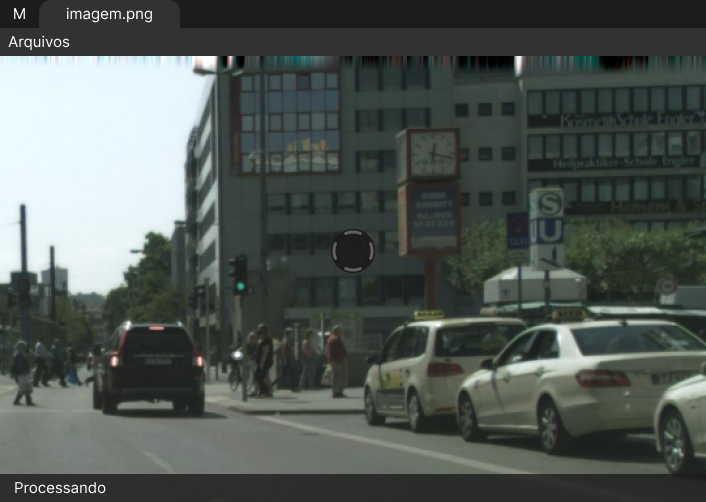
\includegraphics[width=0.6\textwidth]{figures/tela_processando_1.png}
    \legend{Fonte: Criação própria}
	\label{fig:tela_processando_1}
\end{figure}


\begin{figure}[H]
	\centering
    \caption{Tela de seleção de segmentação da imagem.}
	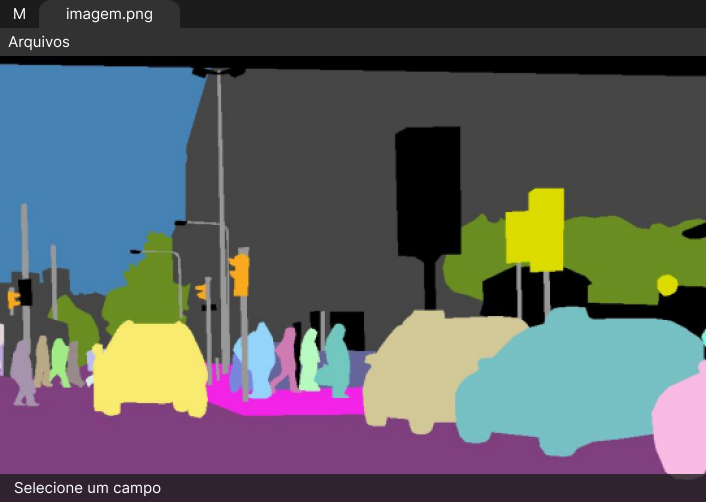
\includegraphics[width=0.6\textwidth]{figures/tela_carregado.png}
    \legend{Fonte: Criação própria}
	\label{fig:tela_carregado}
\end{figure}


\begin{figure}[H]
	\centering
    \caption{Tela de processamento para geração do mapa com a seleção do segmento.}
	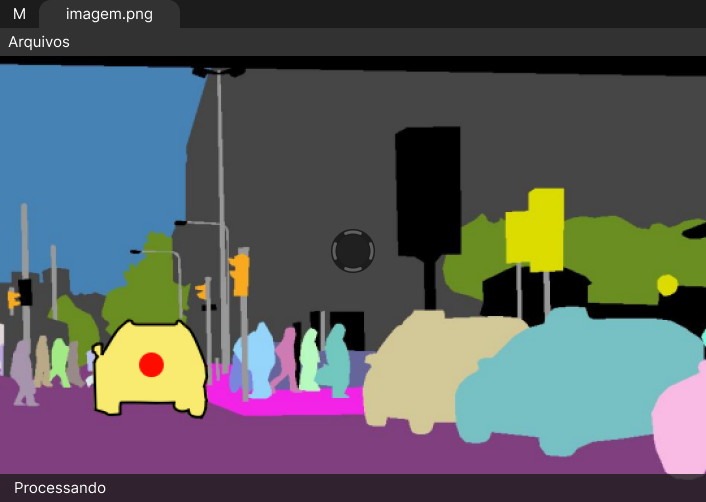
\includegraphics[width=0.6\textwidth]{figures/tela_processando_2.png}
    \legend{Fonte: Criação própria}
	\label{fig:tela_processando_2}
\end{figure}


\begin{figure}[H]
	\centering
    \caption{Tela de resultado com o mapa gerado após processamento.}
	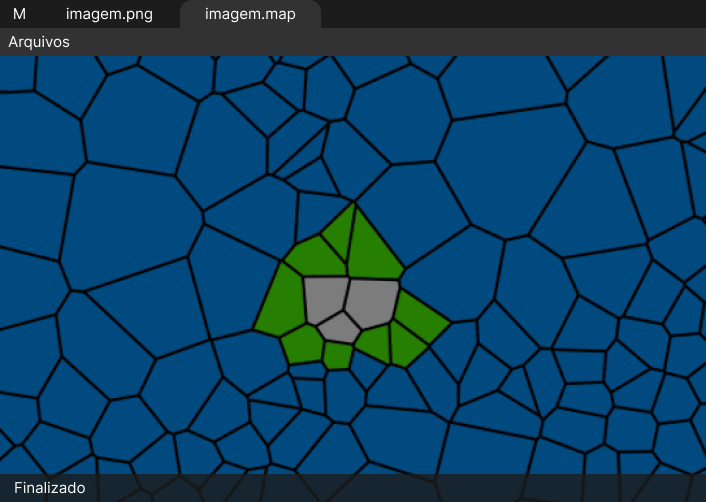
\includegraphics[width=0.6\textwidth]{figures/tela_mapa.png}
    \legend{Fonte: Criação própria}
	\label{fig:tela_mapa}
\end{figure}

Após isso a interface permitirá o usuário salvar o projeto bem como exportar o resultado.

O tempo de desenvolvimento será em torno de 1 mês.
% ----------------------------------------------------------
% Finaliza a parte no bookmark do PDF
% para que se inicie o bookmark na raiz
% e adiciona espaço de parte no Sumário
% ----------------------------------------------------------
%\phantompart

% ---
% Conclusão (outro exemplo de capítulo sem numeração e presente no sumário)
% ---
% \chapter*[Conclusão]{Conclusão}
% \addcontentsline{toc}{chapter}{Conclusão}
% ---

% \lipsum[31-33]

% ----------------------------------------------------------
% ELEMENTOS PÓS-TEXTUAIS
% ----------------------------------------------------------
\postextual
% ----------------------------------------------------------

% ----------------------------------------------------------
% Referências bibliográficas
% ----------------------------------------------------------
\bibliography{references}

% ----------------------------------------------------------
% Glossário
% ----------------------------------------------------------
%
% Consulte o manual da classe abntex2 para orientações sobre o glossário.
%
%\glossary

% ----------------------------------------------------------
% Apêndices
% ----------------------------------------------------------

% ---
% Inicia os apêndices
% ---
% \begin{apendicesenv}

% % Imprime uma página indicando o início dos apêndices
% \partapendices

% % ----------------------------------------------------------
% \chapter{Quisque libero justo}
% % ----------------------------------------------------------

% \lipsum[50]

% % ----------------------------------------------------------
% \chapter{Nullam elementum urna vel imperdiet sodales elit ipsum pharetra ligula
% ac pretium ante justo a nulla curabitur tristique arcu eu metus}
% % ----------------------------------------------------------
% \lipsum[55-57]

% \end{apendicesenv}
% ---


% ----------------------------------------------------------
% Anexos
% ----------------------------------------------------------

% ---
% Inicia os anexos
% ---
% \begin{anexosenv}

% % Imprime uma página indicando o início dos anexos
% \partanexos

% % ---
% \chapter{Morbi ultrices rutrum lorem.}
% % ---
% \lipsum[30]

% % ---
% \chapter{Cras non urna sed feugiat cum sociis natoque penatibus et magnis dis
% parturient montes nascetur ridiculus mus}
% % ---

% \lipsum[31]

% % ---
% \chapter{Fusce facilisis lacinia dui}
% % ---

% \lipsum[32]

% \end{anexosenv}

%---------------------------------------------------------------------
% INDICE REMISSIVO
%---------------------------------------------------------------------
%\phantompart
\printindex
%---------------------------------------------------------------------

\end{document}